\documentclass[11pt,a4paper]{report}		                                   

\usepackage{amsmath}
\usepackage[utf8]{inputenc}
\usepackage{graphicx}
\usepackage{multicol} 
\usepackage{subfig}
\usepackage{float}
\usepackage{nameref}
\usepackage{amssymb}
\usepackage{gensymb}
\usepackage[round]{natbib}
\usepackage{listings}
\usepackage{url}
\usepackage{aliascnt}
\usepackage[table]{xcolor}
\usepackage[bottom]{footmisc}
\usepackage[ngerman]{babel}
\usepackage{microtype}
\usepackage{hyperref}
\usepackage{hypcap}
\hypersetup{pdftex,colorlinks=true,allcolors=black}

\definecolor{dkgreen}{rgb}{0,.6,0}
\definecolor{dkblue}{rgb}{0,0,.6}
\definecolor{dkyellow}{rgb}{.5,.4,0}

\lstset{
  language        = c++,
  basicstyle      = \small\ttfamily,
  keywordstyle    = \color{dkblue},
  stringstyle     = \color{red},
  identifierstyle = \color{black},
  commentstyle    = \color{gray},
  emph            =[1]{php},
  emphstyle       =[1]\color{black},
  emph            =[2]{if,and,or,else, var, then, set},
  emphstyle       =[2]\color{dkyellow}}

\newaliascnt{eqfloat}{equation}
\newfloat{eqfloat}{h}{eqflts}
\floatname{eqfloat}{Equation}

\newcommand*{\ORGeqfloat}{}
\let\ORGeqfloat\eqfloat
\def\eqfloat{%
  \let\ORIGINALcaption\caption
  \def\caption{%
    \addtocounter{equation}{-1}%
    \ORIGINALcaption
  }%
  \ORGeqfloat
}
\parindent 0em

\bibliographystyle{bst_styles/apalike_german}

\newcommand{\thema}{Methoden des Deep Learning im Bereich Convolutional Neural Networks}
\newcommand{\schlagworte}{Machine Learning, Deep Learning, Convolutional Neural Network, Convolutional Autoencoder, Backpropagation, Gradient Descent, Regularization, Visualization MNIST, CIFAR-10}

\newcommand{\zusammenfassung}{
This thesis deals with Convolutional Neural Networks (CNNs) and their application in Deep Learning. CNNs represent a special case of Neural Networks which assume that the inputs have local features. These assumptions allow to encode certain properties into the architecture and make CNNs the state-of-the-art technology for image recognition, speech recognition and natural language processing. CNNs are Neural Network with special Convolution- and Pooling-Layers in the first layers for implicit feature extraction. Based on these features the last layers of the neural network perform classification or regression tasks. The new field of Deep Learning provides some very useful methods and tricks to address the difficulties in training such deep Neural Networks with Backpropagation. These tackle mainly the so called vanishing gradient effect and issues in optimazation of non-convex cost functions. Within the frame of this thesis the development of a CNN library is being described. It reaches a test error of 0.61 \% on MNIST respectively 25.02 \% on CIFAR-10 and provides most of the current techniques as Max-Pooling, Dropout training, unsupervised pre-training and visualization of features. Further it contains recent gradient descent acceleration methods as Equilibrium SGD, Nesterov-Momentum, RMSprop and AdaDelta.
}


\newcommand{\ausgabedatum}{01.04.2015}
\newcommand{\abgabedatum}{30.09.2015}
\newcommand{\autor}{Matthias Hermann}
\newcommand{\autorStrasse}{Zimmererweg 3}
\newcommand{\autorPLZ}{78467} 
\newcommand{\autorOrt}{Konstanz}
\newcommand{\autorGeburtsort}{Wangen im Allgäu}
\newcommand{\autorGeburtsdatum}{04.12.1988}
\newcommand{\prueferA}{Prof. Dr. Matthias O. Franz}
\newcommand{\prueferB}{Martin Schall, M. Sc.}
\newcommand{\firma}{HTWG Konstanz}
\newcommand{\studiengang}{Master of Science, Informatik}
\newcommand{\danksagung}{
F\"ur die wissenschaftliche Betreuung meiner Masterarbeit und die interessanten und motivierenden Besprechungen m\"ochte ich mich herzlich bei Prof. Dr. Matthias Franz bedanken. Ein herzlicher Dank geht auch an Martin Schall für die Erstellung des Zweitgutachtens sowie die vielen aufschlussreichen Diskussionen.\newline \newline
Dank gilt außerdem Michael Grundwald für die Durchsicht meiner Arbeit und die zahlreichen konstruktive Vorschl\"age. \newline \newline
Ganz herzlich m\"ochte ich mich schließlich bei ZF Friedrichshafen AG und insbesondere bei Timo Möllers, Andreas Bauer und Wolfgang Duttle bedanken. Diese erm\"oglichten mir das Studium und standen w\"ahrend meines gesamten Masterstudiums unterst\"utzend zur Seite.
}
 
\begin{document} 
 
\pagenumbering{Roman}

\begin{titlepage}
\vspace*{-3.5cm}
 \begin{flushleft}
 \hspace*{-1cm} 
\includegraphics[width=15.7cm]{images/htwg-logo}
 \end{flushleft}
\vspace{2.5cm}
\begin{center}
	\huge{
		\textbf{\thema} \\[5cm]
	} 
	\Large{
		\textbf{\autor}} \\[6.5cm]
	\large{
		\textbf{Konstanz, \abgabedatum} \\[2.3cm]
	}
	
	\Huge{
		\textbf{{\sf MASTERARBEIT}}
	}
\end{center}
\end{titlepage}

\begin{center}
\setlength{\parskip}{0.5cm}
\textbf{\huge MASTERARBEIT}

\textbf{zur Erlangung des akademischen Grades}

\textbf{\Large Master of Science (M. Sc.)}

\textbf{an der}

\textsf{\huge Hochschule Konstanz}\\
{\small Technik, Wirtschaft und Gestaltung}

\textsf{\Large Fakultät Informatik} \\
{Studiengang \studiengang}

\vfill

\begin{tabular}{p{3cm}p{10cm}}
	Thema: 			& \textbf{\large \thema} \\[15ex]
	Masterkandidat: & \autor, \autorStrasse, \autorPLZ\ \autorOrt \\[15ex]
	1. Prüfer: 		& \prueferA \\
	2. Prüfer: 		& \prueferB \\[25ex]
	Ausgabedatum: 	& \ausgabedatum \\
	Abgabedatum: 	& \abgabedatum \\
\end{tabular}

\end{center}

\newpage
\begin{center}
%\addcontentsline{toc}{chapter}{Abstract}
{\Large \textbf{Abstract}}
\end{center}
\bigskip

\begin{center}
	\begin{tabular}{p{2.8cm}p{10cm}}
		Thema: & \thema \\
		 & \\
		Masterkandidat: & \autor \\
		 & \\
		Firma: & \firma \\
		 & \\
		Betreuer: & \prueferA  \\[.5ex]
		 &  \prueferB \\
		 & \\
		Abgabedatum: & \abgabedatum \\
		 & \\
		Schlagworte: & \schlagworte \\
		 & \\
	\end{tabular}
\end{center}

\bigskip

\noindent
\zusammenfassung

\newpage
\begin{center}
%\addcontentsline{toc}{chapter}{Ehrenwörtliche Erklärung}
{\Large \textbf{Ehrenwörtliche Erklärung}}
\end{center}
\bigskip
Hiermit erkläre ich
\textit{\autor, geboren am \autorGeburtsdatum\ in \autorGeburtsort}, dass ich\\

\begin{tabular}{lp{12cm}}
(1) & meine Masterarbeit mit dem Titel \\[1em]
& \textbf{\thema} \\[1em]
& bei der \firma\ unter Anleitung von \prueferA\ selbständig und ohne fremde Hilfe 
angefertigt und keine anderen als die angeführten Hilfen benutzt habe;\\[1em]
(2) & die Übernahme wörtlicher Zitate, von Tabellen, Zeichnungen, Bildern und
Programmen aus der Literatur oder anderen Quellen (Internet) sowie die Verwendung
der Gedanken anderer Autoren an den entsprechenden Stellen innerhalb der Arbeit
gekennzeichnet habe.\\
\end{tabular}

\vspace*{1cm}

\noindent
Ich bin mir bewusst, dass eine falsche Erklärung rechtliche Folgen haben wird.\\

\vspace*{3cm}

\noindent
Konstanz, \abgabedatum \hfill \begin{tabular}{c} \\ \\ \rule{5cm}{1pt} \\ (Unterschrift)\end{tabular}

\newpage
\begin{center}
\addcontentsline{toc}{chapter}{Danksagung}
{\Large \textbf{Danksagung}}
\end{center}
\bigskip
\danksagung

\tableofcontents
\addcontentsline{toc}{chapter}{Inhaltsverzeichnis}
\newpage
\pagenumbering{arabic}    

\chapter{Einleitung}
\label{ch:Einleitung}
Maschinelles Lernen stellt den Oberbegriff für Computerprogramme dar, welche hinsichtlich eines Performanzmaßes P (\textit{Performance Measure}) eine Aufgabe A mit zunehmender Erfahrung E besser lösen können. Erfüllt ein Programm diese Anforderung wird es als lernend bezeichnet \cite[vgl.][S. 2]{Mitchell1997}.
Die verschiedenen Teilgebiete dieser Disziplin unterscheiden sich in der Struktur der Aufgabe A sowie des auf die Erfahrung beziehungsweise Trainingsdaten angewandten Lernverfahrens. Seit der Erfindung des Computers wurden so eine Vielzahl verschiedener Modelle entwickelt \cite[vgl. z.B.][]{Hastie2009}. Ganz allgemein können diese Modelle in vier  Gruppen aufgeteilt werden. Diese entsprechen den verschiedenen Anwendungsgebiete des maschinellen Lernens und sind in Tabelle \ref{tab:ml} aufgeführt.\\
\begin{table}[H]
\centering
\begin{tabular}{c|c}
Klassifikation  & Regression \\ 
\hline  Dichteschätzung & Rangfolgebestimmung \\ 
\end{tabular}
\caption{Die verschiedenen Methoden im maschinellen Lernen \cite[vgl.][S. 1 f.]{Hastie2009}} 
\label{tab:ml} 
\end{table}

Ein weiteres integrales Merkmal eines Models im maschinellen Lernen ist das angewandte Lernverfahren, auch Lernparadigma genannt (vgl. hierzu und im Folgenden \cite{Haykin1999}, S. 63 ff. und \cite{Becker1991}).
\begin{itemize}
\item Überwachtes Lernen (\textit{Supervised learning}): Die Trainingsdaten $D_1 =\{(x_1,y_1),..,(x_n,y_n)\}$ liegen in Eingabe-Ausgabe-Beispielen vor, mit dem Ziel die Abbildung von Ein- nach Ausgabe beziehungsweise Trainingsbeispiel $x_i$ und Label $y_i$ zu lernen.
\item Unüberwachtes Lernen (\textit{Unsupervised learning}): Die Trainingsdaten $D_2 =\{(x_1),..,(x_n)\}$  liegen ohne Labels vor. Das Modell lernt statistische Merkmale der Daten und somit eine interne Repräsentation.
\item Bekräftigungslernen (\textit{Reinforcement learning}): Hierbei wird ebenfalls eine Abbildung von Ein- nach Ausgabe gelernt. Allerdings erhält das System lediglich zeitlich verzögert Rückmeldung über die Performanz der Abfolge von Ausgaben. Ziel ist es, hinsichtlich eines skalaren Performanzmaßes optimale Ausgaben zu erzeugen. 
\end{itemize}


\section{Deep Learning}
\label{ch:DeepLearning}
Moderne Lernalgorithmen wie Support Vector Machines (SVMs) bieten viele interessante Eigenschaften, wie Schlupfvariablen, maximale Trennbreite und eine konvexe Kostenfunktion. Analysen der letzten Jahre zeigen jedoch, dass solche modernen parameterlosen Lernalgorithmen fundamentalen Restriktionen unterliegen \cite[vgl. hierzu und im Folgenden][]{Bengio2007b}.

Zum einen ruhen diese auf einem dem \textit{Fluch der Dimensionalität} sehr ähn\-lichen Problem \cite[siehe][]{Duda73}. Außerdem auf der Berechnung der lokalen Ähnlichkeit (Euklidischen Distanz) einer neuen Eingabe zu bereits bekannten Beispielen. Kern-basierte Verfahren mit lokalem Kern, wie dem Gauß-Kern, arbeiten unter der Annahme, dass die Zielfunktion glatt ist und verwandte Daten im Eingaberaum einer gewissen Ähnlichkeit unterliegen. Dies ist beispielsweise nicht mehr gegeben, wenn verwandte Daten in veränderter Form, wie affin transformiert, in unterschiedlichen Ausprägungen oder verstärkt, vorliegen. Nach \cite{Bengio2007b} erfordert das Lernen von Funktionen mit großen Variationen im Eingaberaum ebenso viele Trainingsdaten, was in Verbindung zum \textit{Fluch der Dimensionalität} steht. Des weiteren können Verfahren, welche auf lokaler Generalisierung beruhen, nicht zwischen relevanten und irrelevanten Merkmalen (z. B. Vorder- und Hintergrund) unterscheiden, was gerade in der Bilderkennung zu erheblichen Beschränkungen führt. Wünschenswert ist somit ein Verfahren, das nicht lokal generalisiert und mit steigender Anzahl Trainingsdaten (mehrere 10.000) gut skaliert.

Ein Lösungsansatz, um sehr komplexe Funktionen kompakt mit wenigen Parametern darzustellen, ist die Kombination vieler nicht-linearer Funktionen in Form der Gleichung \ref{eq:fx}.
\begin{equation}
\label{eq:fx}
f(x) = f''(f'(x))
\end{equation}
Dies ermöglicht es den Eingaberaum in unterschiedlichen Abstraktionsebenen zu partitionieren und so eine verteilte Repräsentation der Eingabe zu formen (\textit{Distributed Representation}) \cite[vgl.][]{Rumelhart1986b}. So können nicht-lokale Merkmale und große Variationen im Eingaberaum abgebildet werden, was gerade im Bereich Bildverarbeitung, natürliche Sprache und Robotik von großer Relevanz ist. Durch die Wahl eines parametrisierten Modells kann das Modell darüber hinaus mit steigender Anzahl Trainingsdaten skalieren \textemdash Derartige Modelle heißen Künstliche Neuronale Netze (KNNs) \cite[vgl.][]{McCulloch1943}.\\
Angetrieben von der architektonischen Tiefe biologischer Gehirne, obgleich kein Beleg für eine derartige Funktionsweise dieser existiert \cite[vgl.][]{Becker1991}, wurde so in der Vergangenheit oftmals versucht tiefe Netze (DNNs) überwacht zu trainieren (\textit{Deep Learning}). Allerdings mit bedingtem Erfolg \cite[vgl.][]{Bengio2007b}. Denn trotz der Ausdrucksstärke tiefer Modelle, stellt das Training solcher eine enorme Schwierigkeit dar \cite[vgl.][]{Becker1991}. Oft genannte Gründe stehen in Zusammenhang mit zufälliger Initialisierung der Parameter und der Optimierung nicht-konvexer Zielfunktionen, welche durch viele Plateaus und lokalen Minima charakterisiert sind \cite[vgl.][]{Bengio2009}.
Bis auf bemerkenswerte Erfolge sogenannter \textit{Convolutional Neural Networks} \cite[vgl.][]{LeCun1989} sind somit tiefe Architekturen in der Vergangenheit weitestgehend unbeachtet geblieben.

\subsubsection{Renaissance durch Vortraining}
\begin{figure}
\centering
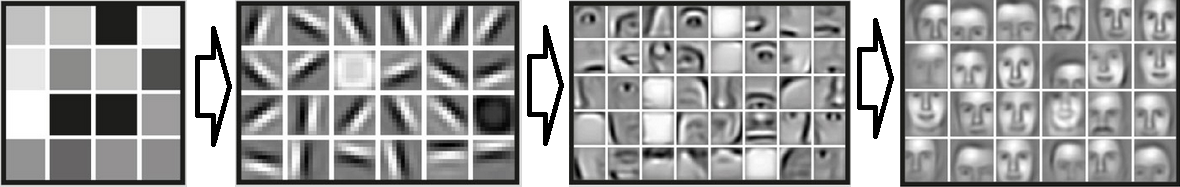
\includegraphics[width=0.95\linewidth]{images/1_Features}
\caption[Merkmale unterschiedlichen Abstraktionsgrads von links (Pixel) bis rechts (Gesichter)]{Merkmale unterschiedlichen Abstraktionsgrads von links (Pixel) bis rechts (Gesichter) (Einzelbilder: Andrew Ng, Stanford Artificial Intelligence Lab)}
\label{fig:1_Features}
\end{figure}
Den Beginn des heutigen Deep Learning stellt die Arbeit von \cite{Hinton2006} dar: Ein unüberwachtes Lernverfahren, welches tiefe Architekturen schichtweise mittels eines \textit{Greedy}-Algorithmus trainiert. Dadurch können, wie in Abbildung \ref{fig:1_Features} dargestellt, unterschiedliche Schichten Merkmale mit unterschiedlichem Abstraktionsgrad extrahieren. Die Gesamtstrategie sieht dabei vor, zuerst Merkmale unüberwacht zu extrahieren und diese im Anschluss für ein etwaiges überwachtes Lernverfahren, wie beispielsweise Kern-basierte Verfahren \cite[vgl.][]{Salakhutdinov2008}, zu verwenden. Dies ähnelt stark den Ideen von \cite{Becker1991}, die Principle Component Analysis (PCA) zur Vorverarbeitung der Trainingsdaten zu verwenden. Durch die tiefe, schichtweise Extraktion der Merkmale sind diese jedoch nicht exklusiv, sondern verteilt, was auch als \textit{Distributed Representation} bezeichnet wird \cite[vgl.][]{Hinton1986}.

In den vergangenen Jahren konnten so bahnbrechende Fortschritte im Bereich der Spracherkennung \cite[vgl][]{Sainatha2015}, der Verarbeitung natürlicher Sprache (NLP) \cite[vgl.][]{Socher2011} sowie  der Bilderkennung erzielt werden. Den aktueller Benchmark in Letzterem stellt das \textit{GoogLeNet} von \cite{Szegedy14} mit $26\%$ Top-5 Fehlern auf dem bekannten ImageNet-Problem\footnote{Der ImageNet-Datensatz besteht aus 200 Klassen, rund 450.000 Trainingsbeispielen, rund 20000 Beispielen zur Validierung und rund 40.000 Testbeispielen. Jedes Bild hat eine Größe von $482 \times 415 $  (\url{http://www.image-net.org/} (26.08.2015)).} \cite[vgl.][]{ImageNet2015}. Von den neuen Möglichkeiten im \textit{Deep Learning} profitieren auch die im letzten Kapitel erwähnten \textit{Convolutional Neural Networks} insofern, dass bestehende Ideen weiterentwickelt oder fehlende gelabelte Trainingsdaten kompensiert werden \cite[vgl.][]{LeRanzato2012}.\\

Heute werden unter \textit{Deep Learning} meist folgende fünf Modelle unterschieden:
\begin{itemize}
\item \textit{Recurrent Neural Network} (RNN) mit Long Short Term Memory (LSTM) (vgl. \cite{Hochreiter1997}
\item \textit{Convolutional Neural Network} (CNN)
	(vgl. \cite{LeCun1998}, \cite{Krizhevsky2012} und \cite{Simonyan2014})
\item \textit{Deep Belief Network} (DBNs) mit beschränkten Boltzmann-Maschinen (RBMs) 
	(vgl. \cite{Bengio2007} und \cite{Ranzato2007b})%Real valued
\item \textit{Stacked Denoising Autoencoder} (SDA) 
	(vgl. \cite{Vincent2008} und \cite{Vincent2010})
\item \textit{Deep Reinforcement Learning} (DRL) (vgl. \cite{Mnih2013})
\end{itemize}

\section{Ziel der Arbeit}
\label{ch:Ziele}
\textit{Convolutional Neural Networks} (CNNs) sind eine besondere Klasse von Neuronalen Netzen. Diese von der Neurobiologie inspirierten Modelle in Verbindung mit neueren Methoden aus dem Bereich \textit{Deep Learning}, stellen derzeit die besten Systeme für viele Probleme aus Bilderkennung, Spracherkennung und Verarbeitung natürlicher Sprache. 
Grundsätzlich werden drei Typen klassischer neuronaler Netze unterschieden: \textit{Single-Layer Feedforward Networks}, \textit{Multilayer Feedforward Networks} und \textit{Recurrent Networks} \cite[vgl.][S. 22f]{Haykin1999}, wobei rekurrente Varianten in dieser Arbeit nicht weiter betrachtet werden.

Diese Arbeit beschränkt sich auf \textit{Feedforward Networks} in den Bereichen Klassifikation und Regression und beschreibt somit das klassische, überwachte, neuronale Lernmodell.
Für den Entwurf dieser neuronalen Netze existieren bereits eine Vielzahl an Softwaretools. Als Beispiel werden hier folgende bekannten Softwareprodukte angeführt:
\begin{itemize}
\item Theano (Python) \cite[vgl.][]{Bergstra2010}

\item Torch (Lua) \cite[vgl.][]{Torch2011}

\item Cuda-Convnet (Cuda) \cite[vgl.][]{Nouri2013}

\item PyLean2 (Python) \cite[vgl.][]{PyLearn22013}

\item Caffe (C/C++) \cite[vgl.][]{Caffe2014}
\end{itemize}

Ziel dieser Arbeit ist es zum einen die Methoden im Bereich \textit{Deep Learning} aufzubereiten und zu analysieren. Darauf aufbauend wird ein eigener funktionierender Prototyp eines \textit{Convolutional Neural Networks} entwickelt. Dieser soll möglichst effizient sein, wenige Abhängigkeiten haben sowie eine Python-Schnittstelle bereitstellen. Im Zentrum der Untersuchungen stehen dabei überwachte Lernverfahren mit dem Ziel, Bilddaten mit \textit{State of the Art}-Performance zu klassifizieren, was allgemein als Bilderkennung bezeichnet wird. Darüber hinaus werden Methoden zum unüberwachten Vortraining und zur Visualisierung neuronaler Netze untersucht und vorgestellt.


Diese Arbeit entsteht am Institut für Optische Systeme (IOS) der HTWG Konstanz und dient zusammen mit zwei weiteren Arbeiten im Bereich \textit{Stacked Denoising Autoencoder} und \textit{LSTM-Recurrent Neural Network} als Grundlage für weitere Aktivitäten im Bereich \textit{Deep Learning} im IOS.


\section{Kapitelübersicht}
Diese Thesis ist unterteilt in sechs Kapitel. Kapitel 1 beginnt mit der thematischen Einordnung dieser Arbeit sowie der Motivation. Der Hauptteil ist in zwei Blöcke unterteilt. In Kapitel 2 und 3 werden notwendige Grundlagen für die Implementierung des Prototyps vorgestellt. So führt Kapitel 2 die Methode Neuronale Netze ausgehend vom Perzeptron ein und beschreibt im Speziellen die Besonderheiten der \textit{Convolutional Neural Networks} (CNNs). In Kapitel 3 werden spezielle Methoden des \textit{Deep Learning} vorgestellt. Der zweite Block besteht aus Kapitel 4 und 5. Kapitel 4 beschreibt die Entwicklung des Prototyps und Kapitel 5 die verschiedenen durchgeführten Experimente mit dem Ziel den Prototyp auf Richtigkeit zu überprüfen sowie verschiedene Aspekte im Deep Learning zu untersuchen. Im abschließenden 6. Kapitel werden die relevanten Ergebnisse der Arbeit nochmals zusammengefasst und ein Ausblick auf über diese Arbeit hinausgehende Aspekte gegeben.


\chapter{Grundlagen Neuronaler Feedforward Netze}
\label{ch:mlp}
Neuronale Netze sind äußerst vielseitig. Inspiriert von Gehirnen von Lebewesen, die  einem komplexen, nichtlinearen, parallelen Computer ähneln, finden sie heute Anwendung in der Modellierung, Zeitreihenanalyse, Mustererkennung und Signalverarbeitung. Eine sehr wichtige Eigenschaft ist hierbei die Möglichkeit, von Eingabedaten beziehungsweise Trainingsdaten überwacht, unüberwacht und bekräftigend zu lernen \cite[vgl.][S. 1]{Haykin1999}. Dies erlaubt einen universellen Einsatz in allen Teilgebieten des maschinellen Lernens (vgl. Kapitel \ref{ch:Einleitung}).
Grundsätzlich werden drei Typen neuronaler Netze unterschieden: \textit{Single-Layer Feedforward Networks}, \textit{Multilayer Feedforward Networks} und \textit{Recurrent Networks} \cite[vgl.][S. 22f]{Haykin1999}. Diese Arbeit beschränkt sich jedoch auf nicht rekurrente \textit{Multilayer Feedforward Networks} in den Bereichen Klassifikation und Regression und beschreibt somit das klassische überwachte, neuronale Lernmodell (siehe Kapitel \ref{ch:Einleitung}).


\section{Perzeptron und Multilayer Perceptron}
\begin{figure}
\centering
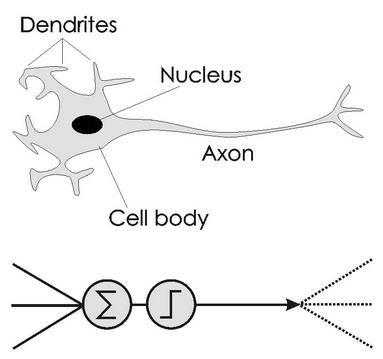
\includegraphics[width=0.4\linewidth]{images/2_neuron}
\caption[Schematischer Vergleich von biologischen und künstlichen \cite{McCulloch1943} Neuronen ]{Schematischer Vergleich von biologischen und künstlichen Neuronen von \cite{McCulloch1943} (nach \cite{Winston1992}, S. 444 ff.)}
\label{fig:2_Neuron}
\end{figure}
Heutige Neuronale Netze basieren auf dem in den späten 1950er von \cite{Rosenblatt1962} entwickelten Perzeptron. Wie Abbildung \ref{fig:2_Neuron} zeigt, ist die Architektur des Perzeptron an biologische Neuronen angelehnt. Die Ausgabe wird berechnet indem die Summe über die Produkte zwischen der Eingabe $x_i$ und den Gewichten $w_i$ gebildet wird. Erreicht die Summe einen definierten Schwellwert (\textit{Bias}) $-b$, wird das Neuron aktiviert und gibt die binäre Eins aus, ansonsten die binäre Null. Formal berechnet das Perzeptron somit die in Gleichung \ref{eq:perceptron} aufgeführte Funktion.
\begin{equation}
\label{eq:perceptron}
f(x) = sign(\sum_{i}^{n} w_ix_i + b) = sign(\langle w, x \rangle + b) 
\end{equation}

Obwohl das Perzeptron sich in dieser Form bereits als linearer Klassifikator eignet, ist es in seiner Ausdrucksstärke sehr eingeschränkt. So ist es beispielsweise nicht möglich Entscheidungshierarchien, wie in Netzwerken von \cite{McCulloch1943}, zu bilden und somit das bekannte XOR-Problem zu lösen.

Die Erweiterung zum Perzeptron stellt das in den 1980er Jahren von \cite{Rumelhart1986b} entwickelte \textit{Multilayer Perceptron} (MLP) dar. Die Architektur eines MLP wird bestimmt durch die Anzahl an Schichten (\textit{Layers}) sowie der pro Schicht enthaltenen Neuronen. Abbildung \ref{fig:2_mlp} zeigt die generische Organisation mehrerer Neuronen in der Eingabeschicht (Input-Layer), der Verdeckten Schicht (Hidden-Layer) und der Ausgabeschicht (Output-Layer). Neuronen verallgemeinern hierbei das Perzeptron insofern, dass diese die Schwellwert-Aktivierungsfunktion durch eine beliebige Funktion $\phi(\cdot)$ ersetzen können. Somit ermöglichen diese auf die reellen Zahlen $\mathbb{R}$ abzubilden. Darüber hinaus kann durch die Darstellung von Entscheidungshierarchien auch das XOR-Problem gelöst werden \cite[vgl.][S. 125]{Rojas1996}. 

Zusammenfassend lässt sich sagen, dass  durch die richtige Wahl der Architektur und Aktivierungsfunktion mit MLPs eine beliebige Funktion $f:\mathbb{R}^n \rightarrow \mathbb{R}^m $ beliebig genau approximiert werden kann, was durch das \textit{Universal Approximation Theorem} beschrieben ist. Die Schwierigkeit besteht jedoch darin, dass die zu approximierende Funktion lediglich durch Trainingsbeispiele gegeben ist und die Gewichte und Schwellwerte durch Training so angepasst werden müssen, dass neue Werte möglichst gut extrapoliert werden (Generalisierung) \cite[vgl.][S. 24 ff.]{Rojas1996}. 

 \begin{figure}[H]
 \centering
 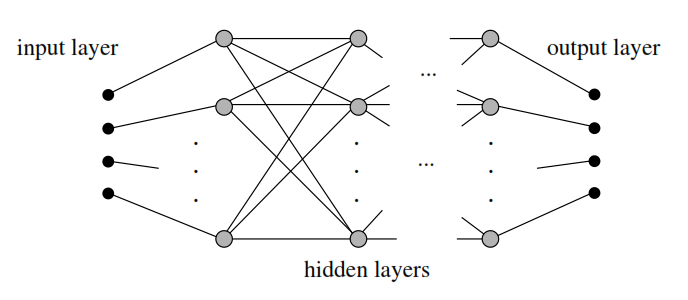
\includegraphics[width=0.8\linewidth]{images/2_mlp}
 \caption[Generische mehrschichtige Architektur eines MLP]{Generische mehrschichtige Architektur eines MLP (siehe \cite{Rojas1996}, S. 126)}
 \label{fig:2_mlp}
 \end{figure}

Ein einfaches Beispiel soll an dieser Stelle die Verbindung zwischen MLP und \textit{Deep Learning} herstellen. Die einfachste Architektur eines MLP umfasst die Eingabe $x$ (Eingabeneuronen), ein \textit{Hidden}-Neuron $w_2$ sowie ein Ausgabeneuron $w_1$. Formal wird diese Architektur durch die Funktion in Gleichung \ref{eq:deep_mlp} beschrieben, welche in unmittelbarer Verbindung zu den in Kapitel \ref{ch:DeepLearning} beschriebenen tiefen Architekturen steht.
\begin{equation}
\label{eq:deep_mlp}
f(x) = \phi(\langle w_1, \phi(\langle w_2, x \rangle + b_2) \rangle + b_1) 
\end{equation}

Analog dazu fusionieren die Gewichtsvektoren $w_i$ bei mehrere Neuronen in einer Schicht zu einer Matrix $ W $ in der die einzelnen $w_i$ der Neuronen zeilenweise organisiert sind. Das innere Produkt in der Gleichung \ref{eq:deep_mlp} wird so durch eine Matrix-Vektor-Multiplikation ersetzt und der skalare Schwellwert $b_i$ mit einem Vektor $b$. Eine Schicht eines MLP kann folglich mit $\phi(Wx + b)$ formal dargestellt werden.

\section{Aktivierungsfunktionen}
\label{ch:aktivierungsfunktonen}
Im letzten Kapitel wurde vorgestellt wie sich das Perzeptron zum Neuron und insgesamt zu einem \textit{Multilayer Perceptron} (MLP) verallgemeinern lässt. In diesem Kapitel werden nun die wichtigsten Aktivierungsfunktionen für neuronale Netze vorgestellt \cite[vgl.][S. 2-17]{Hagan2014}.

\subsubsection{Linear}
Die einfachste Funktion ist die Identitätsfunktion. Diese ist in Abbildung \ref{fig:2_linear} dargestellt.

 \begin{figure}[H]
 \centering
 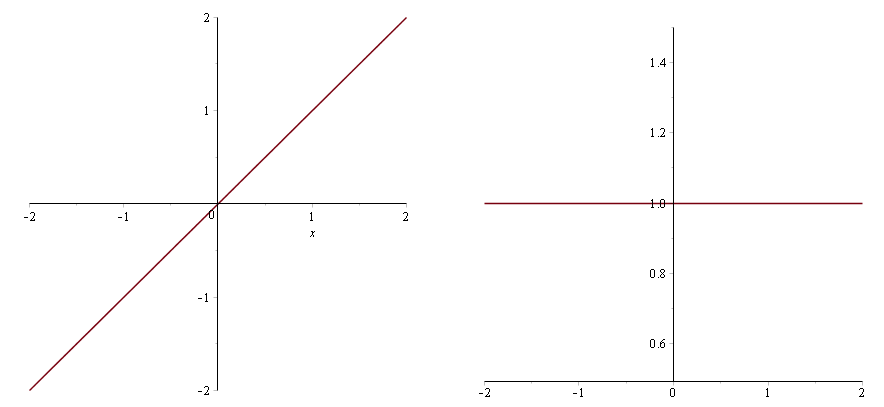
\includegraphics[width=0.6\linewidth]{images/2_linear}
 \caption[Lineare Aktivierungsfunktion und ihre Ableitung]{Lineare Aktivierungsfunktion (links) und Ableitung (rechts)}
 \label{fig:2_linear}
 \end{figure}

\begin{itemize}
\item Funktion:  
\begin{equation} 
f(x) =  x 
\end{equation}
\item Ableitung: 
\begin{equation} 
f'(x) = 1 
\end{equation}
\end{itemize}


\subsubsection{Logistische Sigmoidfunktion}
Ein Spezialfall der Sigmoidfunktion ist die logistische Funktion. Diese nichtlineare Funktion bildet $\mathbb{R} \rightarrow (0,1) $ ab (siehe Abbildung \ref{fig:2_sig}). Eine Besonderheit der Sigmoidfunktion ist, dass die Ableitung an einer bestimmten Stelle durch die Funktion selbst berechnet werden kann.

 \begin{figure}[H]
 \centering
 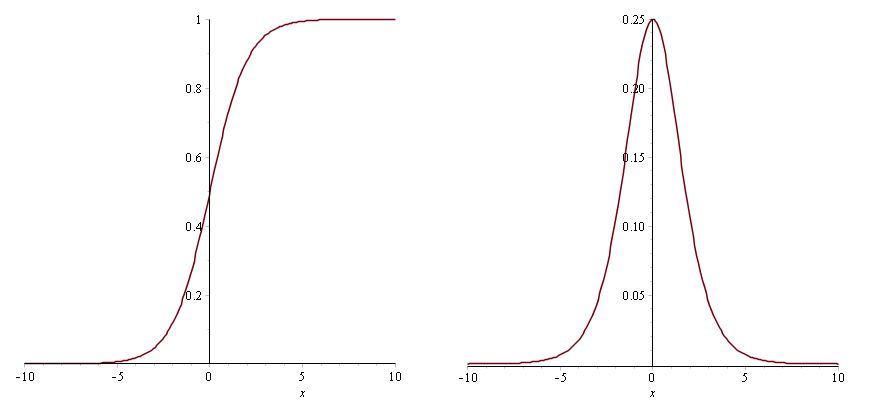
\includegraphics[width=0.6\linewidth]{images/2_sigmoid}
 \caption[Sigmoid Aktivierungsfunktion und Ableitung]{Sigmoid Aktivierungsfunktion (links) und Ableitung (rechts)}
 \label{fig:2_sig}
 \end{figure}
 
 \begin{itemize}
 \item Funktion: 
  \begin{equation} 
 sig(x) = \frac{1}{1 + \exp^{-t}}  
 \end{equation}
 \item Ableitung: 
 \begin{equation} 
 sig'(x) = sig(x)(1-sig(x))
 \end{equation}
 \end{itemize}

\subsubsection{Tangens Hyperbolicus}
Die Tangens Hyperbolicus-Funktion ist eine nichtlineare Funktion, welche $\mathbb{R} \rightarrow (-1,1) $ abbildet (siehe Abbildung \ref{fig:2_tanh}). Wie bei der Sigmoidfunktion, kann die Ableitung an einer bestimmten Stelle ebenfalls durch die Funktion selbst berechnet werden.

 \begin{figure}[H]
 \centering
 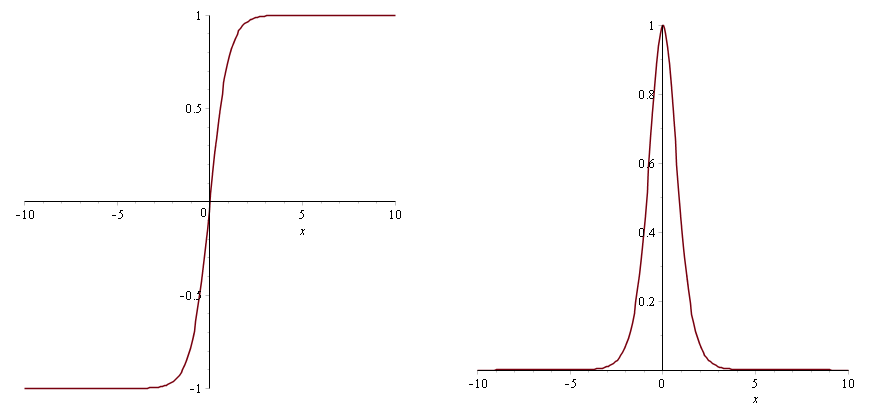
\includegraphics[width=0.6\linewidth]{images/2_tanh}
 \caption[Tangens Hyperbolicus (tanh) Aktivierungsfunktion und Ableitung]{Tangens Hyperbolicus (tanh) Aktivierungsfunktion (links) und Ableitung (rechts)}
 \label{fig:2_tanh}
 \end{figure}
 
  \begin{itemize}
  \item Funktion: 
	  \begin{equation} 
	  tanh(x) = \frac{\exp^x - \exp^{-x}}{\exp^x + \exp^{-x}} 
	  \end{equation}
  \item Ableitung: 
  \begin{equation} 
  	tanh'(x) =1 - tanh(x)^2 
  	\end{equation}
  \end{itemize}

\subsubsection{Rectified Linear}
Die \textit{Rectified Linear}-Funktion (ReLu) ist eine von \cite{Glorot2011} eingeführte Aktivierungsfunktion mit Eigenschaften, die im Bereich der Neuronalen Netze von Interesse sind. So ist bei dieser Aktivierungsfunktion für alle Werte, welche eine von 0 verschiedene Ausgabe erzeugen auch die Ableitung von 0 verschieden. Außerdem können keine negativen Werte auftreten. Die Funktion bildet $\mathbb{R} \rightarrow [0,\infty) $ ab und ist in Abbildung \ref{fig:2_relu} dargestellt.

 \begin{figure}[H]
 \centering
 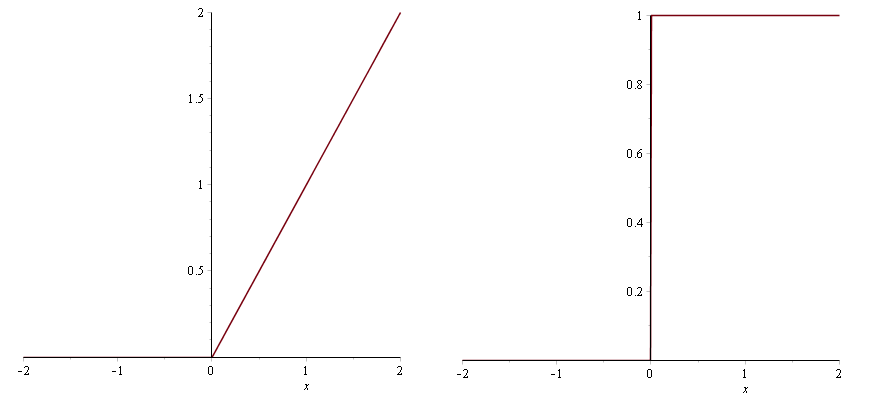
\includegraphics[width=0.6\linewidth]{images/2_relu}
 \caption[Rectified Linear (ReLu) Aktivierungsfunktion und Ableitung]{Rectified Linear (ReLu) Aktivierungsfunktion (links) und Ableitung (rechts)}
 \label{fig:2_relu}
 \end{figure}
 
   \begin{itemize}
   \item Funktion: 
   			\begin{equation} 
   			f(x) =  max(0,x) 
   			\end{equation}
   \item Ableitung: 
   		\begin{equation}
   		   f'(x) =
   		   \begin{cases}
   		     0 & \text{f"ur } 0 \ge x  \\
   		     1 & \text{f"ur } 0 < x
   		     \end{cases}
   		\end{equation}
   \end{itemize}
 

\subsubsection{Softplus}
Die \textit{Softplus}-Funktion ist eine glatte Variante der ReLu-Funktion, welche
 $\mathbb{R} \rightarrow (0,\infty) $ abbildet. Die \textit{Softplus}-Funktion ist in Abbildung \ref{fig:2_sofplus} dargestellt.

 \begin{figure}[H]
 \centering
 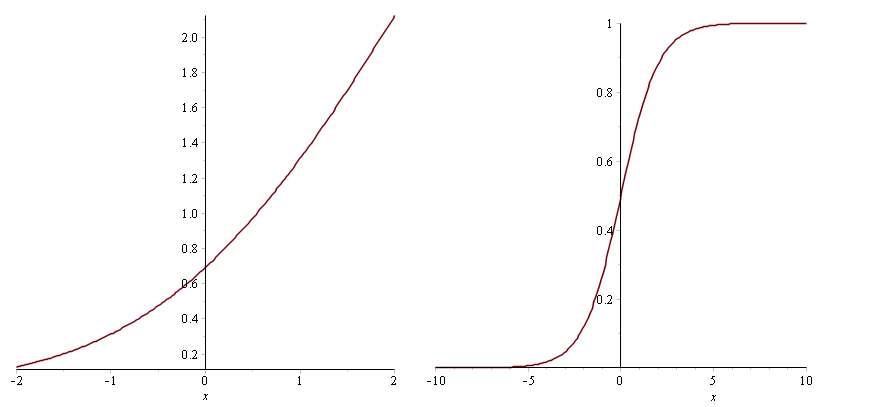
\includegraphics[width=0.6\linewidth]{images/2_softplus}
 \caption[Softplus Aktivierungsfunktion und Ableitung]{Softplus Aktivierungsfunktion (links) und Ableitung (rechts)}
 \label{fig:2_sofplus}
 \end{figure}

 
   \begin{itemize}
   \item Funktion:  
   		\begin{equation} 
   		f(x) =  ln(1+\exp^x) 
   		\end{equation}
   \item Ableitung: 
   	\begin{equation} 
   	f'(x) = \frac{1}{1+\exp^{-x}}
   	\end{equation}
   \end{itemize}

\section{Fehlermaße}
Feedforward-Netze basieren auf dem sogenannten \textit{Error-Correction Learning}. Das bedeutet, dass das Ausgabesignal $y_k$ eines Neuron $k$ (\textit{Output}) des Netzwerks zu einem Eingangssignal $x$ mit einem Zielsignal $d_k$ (\textit{Target})  verglichen und so das Fehlersignal $e_k = d_k - y_k$ erzeugt wird \cite[vgl.][S. 51f]{Haykin1999}.

Um das Fehlersignal in MLPs zu messen, wird ein entsprechendes Fehlermaß benötigt. Dabei werden meist der Mittlere Quadratische Fehler (\textit{Mean Squared Error}) für Regression- und die negative Log-Likelihood (\textit{Cross-Entropy}) für Klassifikationsaufgaben verwendet \cite[vgl.][]{Golik2013}. 

\subsection{Mittlerer Quadratischer Fehler}
Der \textit{Mean Squared Error} (MSE) ist für ein gegebenes MLP $f(x)$ und gegebene Trainingsdaten $D = \{(x_1,y_1),..(x_n,_n)\}$ wie in Gleichung \ref{eq:mse} definiert. Eine Besonderheit stellt der zusätzliche Faktor $\frac{1}{2}$ dar, welcher letztlich aber nur die Ableitung vereinfacht.

 	\begin{equation} 
 	\label{eq:mse}
   	MSE = \frac{1}{2N}\sum_{i}^{N}(f(x_i) - y_i)^2	
   	\end{equation}

\subsection{Cross-Entropy}
Das \textit{Cross-Entropy}-Fehlermaß (CE) ist in Gleichung \ref{eq:cross} dargestellt. Es beschreibt die negative Log-Likelihood über den gesamten Trainingsdaten $D = \{(x_1,y_1),..(x_n,_n)\}$ \cite[vgl.][S. 118]{Mitchell1997}. Als Vorgriff auf Kapitel \ref{ch:gradient} wird hier bereits CE über die Trainingsdaten gemittelt angegeben.

\begin{equation} 
 	\label{eq:cross}
   	CE = - \frac{1}{N}\sum_{i}^{N}(y_i ln(f(x_i)) + (1 - y_i) ln(1 - f(x_i))	
   	\end{equation}

Durch die $ln(\cdot)$-Funktion beachtet CE im Gegensatz zu MSE wie nah das Ausgabesignal am Zielsignal ist, vernachlässigt allerdings im Gegenzug fehlerbehaftete Ausgaben. Dieser Zusammenhang trägt dazu bei, dass CE für Klassifikationsaufgaben besser geeignet erscheint. 


\section{Backpropagation-Algorithmus}
\label{ch:backprop}
In den vergangenen Kapiteln wurden, ausgehend vom Perzeptron, die nichtlinearen MLPs eingeführt und verschiedene Aktivierungsfunktionen vorgestellt. Außerdem wurde gezeigt, dass der Fehler eines Neuronalen Netzes mittels zwei verschiedenen Fehlermaßen angegeben werden kann. Wie im vergangenen Kapitel festgestellt wurde, wird bei Neuronalen Netzen ein sogenanntes \textit{Error-Correction Learning} angewandt. Dazu ist es nötig formal eine Regel zu definieren, mit welcher die Gewichte des Netzwerks verändert werden, um die Performance hinsichtlich des gewählten Fehlermaßes zu optimieren (Gradientenverfahren): Die sogenannte Delta-Regel (vgl. \cite{Widrow1960} und \cite{Widrow1988}. 

Für das Anpassen der Gewichte und Schwellwerte in einem MLP mit nichtlinearen Aktivierungsfunktionen wird eine Verallgemeinerung, der von \cite{Rumelhart1986a} entwickelte Backpropagation-Algorithmus, verwendet. Dieser besteht abstrakt gesehen aus zwei Phasen. In der ersten Phase wird die Ausgabe des Netzes sowie der entsprechende Fehler berechnet (\textit{Forward Pass}), in der zweiten der Fehler mittels Delta-Regel zurück propagiert und so der Gradient schichtweise durch Anwendung der Kettenregel berechnet (\textit{Backward Pass}).

Im Folgenden wird der Backpropagation-Algorithmus vorgestellt \cite[vgl. z.B.][S. 151 ff.]{Rojas1996}. Beispielhaft dient hier der MSE als Fehlermaß.


\begin{multicols}{2}
\begin{itemize}
\item $W^l$: Gewichtsmatrix
\item $b^l$: Vektor mit Schwellwerten
\item $J(\cdot)$: Kostenfunktion
\item $x$: Eingabevektor
\item $x^l$: Layer-Eingabevektor 
\item $f(\cdot)$: Ausgabevektor
\item $\phi(\cdot)$: Aktivierungsfunktion
\item $z^l$: Linearer Ausgabevektor
\item $a^l$: Aktivierter Ausgabevektor
\item $N$: Anzahl Trainingsbeispiele
\item $L$: Anzahl Layer
\item $\circ$: Hadamard-Produkt
\item $\eta$: Lernrate
\end{itemize}
\end{multicols}

Gleichung \ref{eq:backprop0} definiert die Kostenfunktion:
\begin{equation} 
\label{eq:backprop0}
J(W,b) = \frac{1}{2N} \sum_{i=1}^{N}(f(x_i) - y_i)^2	
\end{equation}

Die Gleichungen \ref{eq:backprop1} und \ref{eq:backprop2} beschreiben den allgemeinen Gradientenabstieg:
\begin{equation} 
\label{eq:backprop1}
W_{t+1}^l = W_t - \eta {\nabla W_t} %\frac{1}{N} \sum_{i=1}^{N} \frac{\partial J(W_t,b_t)}
\end{equation}

\begin{equation} 
\label{eq:backprop2}
b_{t+1}^l = b_t - \eta {\nabla b_t} %\frac{1}{N} \sum_{i=1}^{N} \frac{\partial J(W_t,b_t)}
\end{equation}

Der Backpropagation-Algorithmus kombiniert die Delta-Regel mit der Kettenregel und beschreibt so ein Verfahren zur Berechnung der Ableitungen von zusammengesetzten Funktionen. Es wird somit der Gradient für jede Schicht des MLP iterativ berechnet. Um den Gradienten der Kostenfunktion $\nabla J(W,b)$ zu berechnen, wird zuerst für jedes Trainingsbeispiel $\nabla J(W,b,x_i,y_i)$ einzeln berechnet und aufsummiert. Folgende Formeln \ref{eq:backprop3} und \ref{eq:backprop4} beschreiben die Delta-Regeln des Backpropagation-Algorithmus: \\

Delta Output-Layer:
\begin{equation} 
\label{eq:backprop3}
\delta^{L} = (a_i^{L} - y_i) \circ \phi'(z^{L})
\end{equation}

Delta für Hidden-Layer $l$:
\begin{equation} 
\label{eq:backprop4}
\delta^{l} =  ((W^{l+1})^T\delta^{l+1}) \circ \phi'(z^l)
\end{equation}

Die partiellen Ableitungen pro Schicht (Gleichung \ref{eq:backprop5} und \ref{eq:backprop6}) werden über alle Trainingsbeispiele $1..N$ aufsummiert und am Ende eines Durchlaufs mit $\frac{1}{N}$ gemittelt. \\

Partielle Ableitung für Layer $l$:
\begin{equation} 
\label{eq:backprop5}
\frac{\partial J(W,b)}{\partial W^l} = \frac{1}{N} \sum_{i=1}^{N} \delta^{l} (x_i^{l})^T
\end{equation}

\begin{equation} 
\label{eq:backprop6}
\frac{\partial J(W,b)}{\partial b^l} = \frac{1}{N} \sum_{i=1}^{N} \delta^{l}
\end{equation}

Betrachtet man die Delta-Formeln \ref{eq:backprop3} und \ref{eq:backprop4}, wird ersichtlich, dass sich die Verwendung einer Aktivierungsfunktion, deren Ableitung sich durch den Funktionswert selbst berechnen lässt, besonders eignet. Im Falle der Sigmoid-Funktion vereinfacht sich $\phi'(z^l)$ so zu $sig'(z^l) = sig(a^l)(1-sig(a^l))$, was das Speichern von $z^l$ erübrigt.


% Hakin heranführung delta rule	
%	- Backpropagation for gradient computation 			(1 Seite)
%		- derivative of weighting matrix
% 	- Von LMS tu Backpropagation
%   - Beispiel Kettenregel
%Backpropagation ROjas Kaptitel
%
%Bilder
%http://galaxy.agh.edu.pl/~vlsi/AI/backp_t_en/backprop.html



\section{Basisarchitekturen}
Dieses Kapitel beschreibt die zwei Grundarchitekturen Neuronaler Netze (MLPs). Diese umfassen einerseits die  Softmax-Regression zur Klassifikation und andererseits die Nicht\-lineare-Regression.
		
\subsection{Softmax-Regression (Klassifikation)}
\label{ch:softmax}
Die Logistische Regression stellt ein bekanntes lineares statistisches Regressi\-onsverfahren zur Modellierung diskreter abhängiger Variablen dar, welches ursprünglich nichts mit dem Neuronalen Lernmodell zu tun hat. Praktischerweise entspricht dieses jedoch der gleichen Architektur, was die Verwendung als Ausgabeschicht für die Klassifikation mit MLPs nahelegt. Abbildung \ref{fig:2_logistic_regression} zeigt das Verfahren für die diskreten Werte 0 und 1, wobei die Hyperebene zur Visualisierung um $0.5$ verschoben ist.

Allgemein wird mittels des Verfahrens, bei gegebenen Gewichten $W$, die Wahrscheinlichkeit einer binären Ausgabe $y_i \epsilon \{0 ,1\}$ für eine gegebene Eingabe $x_i$ berechnet \cite[vgl. z. B.][S. 119 ff.]{Hastie2009}. 
Die Güte des Models über den gesamten Trainingsbeispielen $N$ kann mit der Formel \ref{eq:logisticRegression} bestimmt werden. Zur Vereinfachung wird von erweiterten Gewichtsvektoren $\hat{w}$ ausgegangen, in denen der Schwellwert $b$ integriert ist.

\begin{figure}
\centering
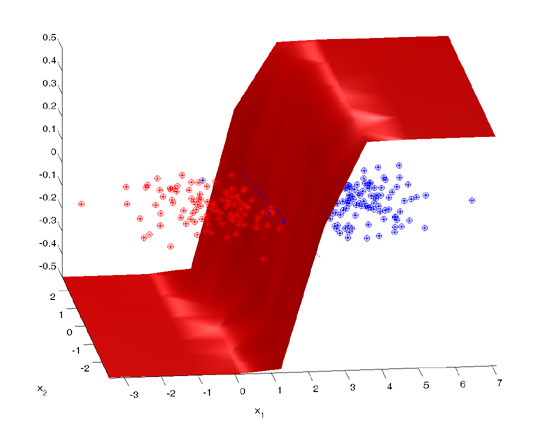
\includegraphics[width=0.5\linewidth]{images/2_logistic_regression}
\caption[Logistische Regression mit zwei Klassen]{Logistische Regression mit zwei Klassen (Bild: Vadim Strijov, Computing Centre of the Russian Academy of Sciences)}
\label{fig:2_logistic_regression}
\end{figure}


\begin{equation} 
\label{eq:logisticRegression}
p(y|X,\hat{W}) = \prod_{i=1}^N [\frac{1}{1 + \exp^{-\hat{W}x_i}} ]^{y_i}  [1 - \frac{1}{1 + \exp^{-\hat{W}x_i}} ]^{1-y_i}
\end{equation}

Wird nun die Likelihood maximiert beziehungsweise die negative Log-\-Likeli\-hood minimiert, erhält man die Formel \ref{eq:logisticRegression2} mit $f(x_i) = \frac{1}{1 + \exp^{-\hat{W}x_i}} $. Dies entspricht proportional einem einschichtigen MLP mit Sigmoid-Akti\-vierungs\-funktion sowie \textit{Cross-Entropy}-Fehlermaß und lässt sich somit mittels des Back\-propa\-gation-Algorithmus optimieren. 

\begin{equation} 
\label{eq:logisticRegression2}
- ln(p(y|X,\hat{W})) = - \sum_{i=1}^N  y_i ln(f(x_i)) + (1-y_i) ln(1 - f(x_i))
\end{equation}


\subsubsection{Multinomiale Regression}
Mehrdimensionale Ausgaben können in neuronalen Netzen durch einfaches Hinzufügen von Neuronen zum Output-Layer erzeugt werden. 
Ein gern verwendeter Code, um mehrere Klassen darzustellen, ist der sogenannte \textit{Grand\-mother-Cell}-Code \cite[vgl.][]{LeCun1998}. Hier wird für $d$-Klassen ein $d$-dimensionaler Zielvektor oder erweiterter Labelvektor definiert mit $d_j = 1$ für die Klasse $j$.
Das Modell der Logistischen Regression lässt sich ebenso leicht auf mehrere Klassen erweitern. Dazu muss die Ausgabe, um ein valides probabilistisches Modell zu erhalten, normalisiert werden. Gleichung \ref{eq:logisticRegression3} beschreibt die Kostenfunktion der multinomialen Regression. Diese ist im Bereich Neuronale Netze eher bekannt als Softmax-Regression (vgl. z.B. \cite{Krizhevsky2012} und \cite{Bengio2015}).

\begin{equation} 
\label{eq:logisticRegression3}
- ln(p(y|X,\hat{W})) = - \sum_{i=1}^N  \sum_{j=1}^d 1\{y^i = j \} ln[\frac{\exp^{\hat{w}_j^Tx^i}}{\sum_{l=1}^d\exp^{\hat{w}_l^Tx^i}} ]
\end{equation}


Neben der Softmax-Regression wird teilweise auch ein Output-Layer mit radialen Basisfunktionen (RBFs) verwendet \cite[vgl.][]{LeCun1998}. Dies hat den Vorteil, dass für jede Klasse ein eigener spezifischer Labelvektor definiert werden kann. Ein Nachteil ist jedoch, dass diese Variante die Ausgabe nicht normalisiert und somit nicht probabilistisch interpretiert werden kann. 
Als Basisfunktionen im Hidden-Layer eignen sich RBFs nur sehr bedingt, da diese lokal im Eingaberaum sind und daher sehr viele Einheiten für hochdimensionale Räume benötigt werden \cite[vgl.][]{LeCun1998b}.

\subsubsection{Besonderheit in Verbindung mit Backpropagation}
Wird Backpropagation angewandt, muss im Output-Layer die Ableitung der Aktivierungsfunktion berechnet werden. Gleichung \ref{eq:softmax} zeigt diese für die Softmax-Funktion. $\delta$ entspricht hierbei dem Kronecker-Delta.
\begin{equation} 
\label{eq:softmax}
softmax'(x)_{ij} = softmax(x)_i(\delta_{ij} - softmax(x)_j)
\end{equation}

Dieser Ausdruck ist sehr unhandlich. Es lässt sich allerdings zeigen, dass die Softmax-Regression in Verbindung mit einem \textit{Cross-Entropy}-Fehlermaß die Berechnung von $\delta^L$ nicht erschwert, sondern zu Gleichung \ref{eq:softmax2} vereinfacht  \cite[vgl. z. B.][Kap. 6.3.2, S. 167]{Bengio2015}. \\

Delta Output-Layer:
\begin{equation} 
\label{eq:softmax2}
\delta^{L} = a_i^{L} - y_i
\end{equation}

Dies bietet damit den großen Vorteil, dass $\delta^L$ nur noch vom Fehler abhängt und nicht mehr von der Ableitung der Aktivierungsfunktion und damit die Nichtlinearität am Ausgang nicht gesättigt wird.


\subsection{Funktionsapproximation (Regression)}
Neuronale Netze können beliebige Funktionen $f:\mathbb{R}^n \rightarrow \mathbb{R}^m $ approximieren und so mittels Backpropagation auf beliebige Daten trainiert werden \cite[vgl.][S. 269 ff.]{Rojas1996}. Es ist lediglich darauf zu achten, dass der Wertebereich des Output-Layers zu dem der Labels passt. So werden im Output-Layer meist lineare Aktivierungsfunktionen verwendet. Alternativ können auch die Labels auf den Wertebereich der verwendeten Aktivierungsfunktion skaliert werden.

\begin{figure}
\centering
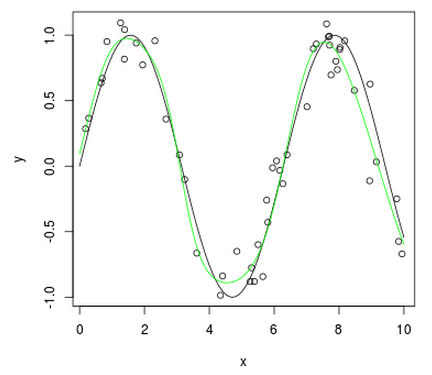
\includegraphics[width=0.5\linewidth]{images/2_sine_nn}
\caption[Approximierte Sinuskurve mit einem Hidden-Layer mit 6 Neuronen (grün)]{Approximierte Sinuskurve mit einem Hidden-Layer mit 6 Neuronen (grün)}
\label{fig:2_sine}
\end{figure}

Abbildung \ref{fig:2_sine} zeigt eine Sinuskurve, welche von einem MLP mit 6 Neuronen im Hidden-Layer approximiert wird. Die zugrundeliegende Trainingsdaten sind aus einer Sinuskurve mit additivem normalverteilten Rauschen generiert. 


\section{Convolutional Neural Networks}
%- Convolutional Neural Networks										( 6 Seiten)
Bildklassifikation, Objektlokalisierung und Objekterkennung rücken derzeit immer mehr in den Fokus. Dies ist beispielsweise an einer immer größeren Verbreitung von Drohnen und autonomen Fahrzeugen zu erkennen ist. Diese Entwicklung geht einher mit den Fortschritten im Bereich Neuronale Netze und den Möglichkeiten des \textit{Deep Learning}. Neuere Arbeiten aus den Neurowissenschaften stützen darüber hinaus getroffene Annahmen mit realen Beobachtungen an Lebewesen, was die Entwicklung weiter unterstützt. In diesem Zusammenhang wird gerne das berühmte \textit{Halle Berry}-Neuron im menschlichen Temporallappen genannt, welches Halle Berry erkennt. Dies deutet darauf hin, dass das biologischen Modell des Sehens auf einem invarianten, dünnbesetzten (\textit{spare}), expliziten Code basiert \cite[vgl.][]{Quiroga2005}.

Dieses Kapitel behandelt eine spezielle Klasse Neuronaler Netze, die das biologische Modell des Sehens und Hörens versuchen zu imitieren. Die sogenannten \textit{Convolutional Neural Networks}.

\subsection{Modellbeschreibung}
\label{ch:cnn_model}
\textit{Convolutional Neural Networks} (CNNs) sind eine Erweiterung des \textit{Multi Layer Perceptrons} (MLPs), welche den biologischen visuellen Cortex zu imitieren versuchen. Die Idee selbst beruht auf den Arbeiten von \cite{Wiesel1962} bezüglich des Sehempfindens von Katzen, die zeigen, dass der visuelle Cortex aus komplex angeordneten Zellen besteht, wobei jede einzelne Zelle einen kleinen Bereich des Sichtfeldes abdeckt. Diese Architektur erlaubt es, räumlich voneinander getrennte Muster zu erfassen. 

Im künstlichen Modell setzt sich ein CNN aus mehreren Convolution- und Pooling-Layern sowie einem klassischen MLP zusammen. Dieses spezielle Design erlaubt es, eine 2D-Struktur im Input-Layer zu erfassen. Dies wird durch sogenannte lokale Verbindungen (\textit{Local Connections}) erzielt.\footnote{Auch wenn die Ursprünge des Modells im Bereich der visuellen Wahrnehmung liegen, wird es heute beispielsweise auch für Spracherkennung und NLP verwendet (vgl. dazu \cite{Socher2011} und \cite{Sainatha2015})}.
Das erste künstliche Modell dieser Art ist das \textit{NeoCognitron} von \cite{Fukushima1980}, welches zwei verschiedene Arten lokaler rezeptiver Felder (siehe Abbildung \ref{fig:3_receptive_field}) definiert: Eines zur Detektion von Kanten und eines mit lokaler Invarianz hinsichtlich Translation. 

 \begin{figure}[H]
 \centering
 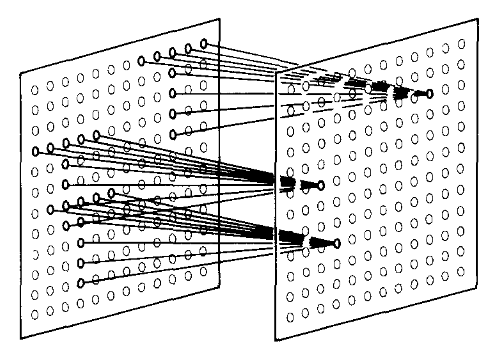
\includegraphics[width=0.3\linewidth]{images/3_receptive_field}
 \caption[Lokales rezeptives Feld]{Lokales rezeptives Feld (siehe \cite{Fukushima1980})}
 \label{fig:3_receptive_field}
 \end{figure}

Das \textit{LeNet} von \cite{LeCun1989} ist die Weiterentwicklung dieses Models. Hier teilen sich mehrere rezeptive Felder dieselben Gewichte beziehungsweise Parameter (\textit{Parameter Sharing}), was die Verbindungen und dadurch auch die Anzahl der Gewichte reduziert. Die Anzahl ist damit von der Dimensionalität der Eingabe entkoppelt. Algebraisch entspricht dies einer Faltung (\textit{Convolution}), wovon das Model seinen Namen ableitet. Diese Architektur ist die Grundlage heutiger CNNs und definiert die damit verbundenen Eigenschaften (vgl. \cite{LeCun1998}, \cite{Bengio2007b} und \cite{Zeiler2014}):
\begin{itemize}
\item Lokale Extraktion von Merkmalen (\textit{Local Feature Extraction})
\item Translationsinvarianz hinsichtlich Eingabedaten (geringe Skalierungs- und Rotationsinvarianz)
\item Einfacheres Training durch weniger Parameter und Verbindungen als MLP mit gleich vielen Neuronen
\item Nicht-lokale Generalisierung durch Verschachtlung nichtlinearer Funktionen
\end{itemize}

Abbildung \ref{fig:3_cnn} stellt ein CNN mit 8 Schichten zur Klassifikation von $32 \times 32$ Pixel großen Eingabebildern dar. Die ersten 6 Schichten zählen zum CNN, während die letzten beiden Schichten ein klassisches MLP repräsentieren. Der zugrundeliegende Ansatz ist hierbei, mittels CNN Merkmale (\textit{Features}) derart zu extrahieren, sodass die Klassen am Ende möglichst gut trennbar sind. 

\begin{figure}[H]
\centering
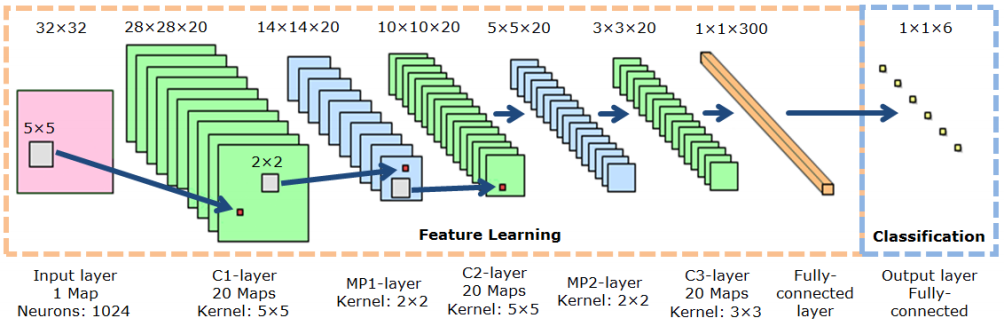
\includegraphics[width=0.95\linewidth]{images/3_CNN_Architecture}
\caption[Convolutional Neural Network mit 8 Schichten]{Convolutional Neural Network mit 8 Schichten \cite[siehe][]{Nagi2011}}
\label{fig:3_cnn}
\end{figure}

Aus Gründen der Vereinfachung werden im weiteren Verlauf des Kapitels lediglich quadratische Eingaben sowie quadratische Filtermasken betrachtet.

\subsubsection{Convolution-Layer}
Der Convolution-Layer ist einer der beiden zentralen Bestandteile eines CNN \cite[vgl. hierzu und im Folgenden][]{LeCun1998}. 
Dieser transformiert eine 3D-Eingabe $x$ mit Tiefe $m$, bezeichnet als $m$-\textit{Input-Maps}, zu einer 3D-Ausgabe $a$. Die Tiefe $n$ der Ausgabe wird bestimmt durch die Anzahl an Faltungskernen und selbst meist als $n$-\textit{Feature-Maps} bezeichnet. Ein Faltungskern $i$ ist in Abbildung \ref{fig:3_cnn_kernel} dargestellt. Er entspricht ebenfalls einer 3D-Struktur, welche durch Höhe $k_h$ und Breite $k_w$ der Faltungsmaske sowie der Tiefe $k_d$ bestimmt ist. Die Tiefe $k_d$ muss der Tiefe der 3D-Eingabe $m$ entsprechen. Es gibt somit gleich viele Faltungsmasken pro \textit{Feature-Map} wie es \textit{Input-Maps} gibt: Es gilt $k_d=m$. Alle Faltungskerne zusammen werden kompakt mit $W$ bezeichnet und einzelne Filtermasken mit $W_{ij}$ eindeutig indiziert.
Wird nun die Netz-Ausgabe (\textit{Forward Pass}) für eine \textit{Feature-Map} $i$ berechnet, muss für jede \textit{Input-Map} $x_j$ die Filtermaske $W_{ij}$ aus dem aktuellen Faltungskern gezogen und die Ausgabe $z_{ij}$ berechnet werden. Dies geschieht mittels diskreter Faltung. Die einzelnen Ausgaben $z_{ij}$ werden über alle \textit{Input-Maps} $1..m$ zu $z_i$ aufsummiert.

Die 3D-Ausgabe $a$ kann auch als Neuronen-Ausgabe interpretiert werden, in welcher jedes Element der Aktivierung eines Neurons entspricht. Bei der Berechnung eines $a_i$ wird folglich zu $z_i$ zunächst ein \textit{Bias} $b_i$ addiert und anschließend die Aktivierungsfunktion $\phi(\cdot)$ berechnet. Dies geschieht elementweise und analog für jede der $n$ \textit{Feature-Maps}.

\begin{figure}[H]
\centering
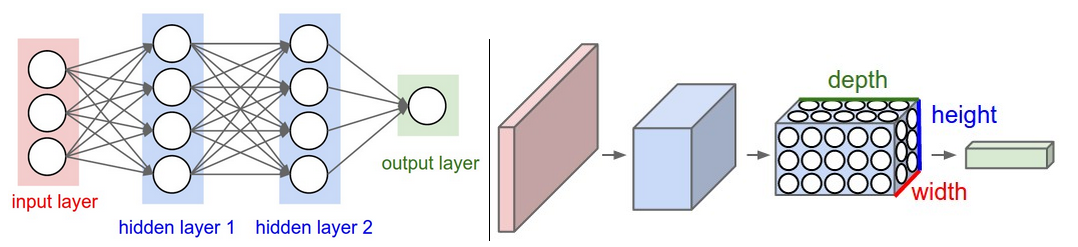
\includegraphics[width=0.95\linewidth]{images/3_cnn_kernel}
\caption[Jeder Convolution-Layer transformiert eine 3D-Eingabe (z.B. RGB-Bild) in eine 3D-Ausgabe]{Jeder Convolution-Layer transformiert eine 3D-Eingabe (z.B. RGB-Bild) in eine 3D-Ausgabe (siehe \cite{Kaparthy2014})}
\label{fig:3_cnn_kernel}
\end{figure}

Folgende Hyperparameter definieren einen Convolution-Layer:
\begin{itemize}
\item \textit{Feature-Maps}: $n$
\item \textit{Input-Maps}: $m = k_d$
\item Größe Faltungskern: $k_w = k_h$
\end{itemize}


Formal berechnet der Convolution-Layer für jede der $n$ \textit{Feature-Maps} zuerst die 2D-Faltung (Faltungsoperator: $\ast$) der $N \times N$-großen $m$ \textit{Input-Maps} mit der Filtermaske $W_{ij}$ (Gleichung \ref{eq:conv}) und im Anschluss elementweise die Aktivierungsfunktion $\phi(\cdot)$. Das Resultat ist die \textit{Feature-Map} $a_i$ (Gleichung \ref{eq:conv2}).
\begin{equation}
\label{eq:conv} 
z_i = \sum_{j=0}^{m}  x_{j} \ast W_{ij}
\end{equation}

\begin{equation}
\label{eq:conv2} 
a_{i} = \phi(z_{i} + b_i)
\end{equation}

Durch die Randbehandlung \textit{valid} reduziert sich die Größe der \textit{Feature-Maps} auf $(N - k_w + 1) \times (N - k_w + 1)$.\footnote{Es existieren bei der Faltung mehrere Modi zur Randbehandlung. Modus \textit{valid} berechnet nur die tatsächlich vorhandenen Elemente, wodurch die Ausgabe in der Größe schrumpft. Im Unterschied dazu berechnet der Modus \textit{full} die Faltung über eine mit Padding versehene Eingabe, wodurch sich die Ausgabe entsprechend vergrößert. Der Modus \textit{same} erzeugt eine gleich große Ausgabe.}

Die Anzahl der Gewichte berechnet sich aus $ n \cdot k_d \cdot k_w \cdot k_w$. Die Anzahl Pixel in der 3D-Ausgabe entspricht der Menge an Neuronen. Im Rahmen des Trainings gilt es, diese Gewichte zu trainieren. Die exakte mathematische Berechnung von Delta  $\delta$ und den partiellen Ableitungen $\frac{\partial J(W,b;x,y)}{\partial W_{ij}^l}$ und $\frac{\partial J(W,b;x,y)}{\partial b_i^l}$ für das Training mit Backpropagation folgt in Kapitel \ref{ch:cnn_back}.

\subsubsection{Pooling-Layer}
Der zweite wichtige Bestandteil eines CNN ist das sogenannte \textit{Pooling}. \cite{LeCun1998} bezeichnen diesen Vorgang als \textit{Subsampling}, wobei heute der Begriff \textit{Pooling} eher geläufig ist (vgl. \cite{Zeiler2013b} oder \cite{Glorot2011}).
Allgemein berechnet der Pooling-Layer ein Downsampling, wobei dessen Art nicht fest definiert ist. Abbildung \ref{fig:3_cnn_subsampling} stellt das sogenannte Max-Pooling dar (vgl. \cite{Glorot2011} und \cite{Zeiler2011}). 
Jede der $m$ \textit{Input-Map} $x_j$ der 3D-Eingabe wird vom Pooling-Layer einzeln bearbeitet und ausgegeben. Die Anzahl $m$ ändert sich nicht und es werden folglich $m$ \textit{Feature-Maps} erzeugt.
Für jedes $x_j$ wird nun ein Bereich der Größe $k_h \times k_w$, wobei $k_h$ der Filterhöhe und $k_w$ der Filterbreite entspricht, ausgeschnitten und verarbeitet. Im Falle des Max-Pooling wird das Maximum berechnet und in der Ausgabe gespeichert.

\begin{figure}[H]
\centering
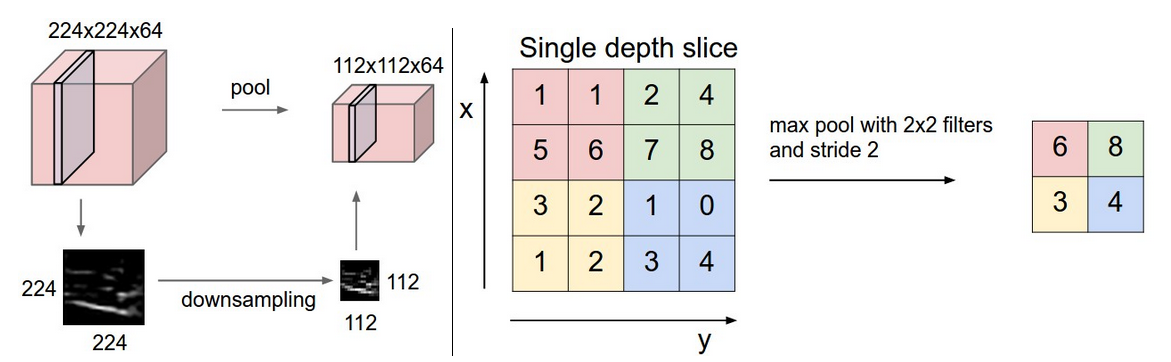
\includegraphics[width=0.95\linewidth]{images/3_cnn_subsampling}
\caption[Ein Pooling-Layer transformiert eine 3D-Eingabe (z.B. RGB-Bild) in eine kleinere 3D-Ausgabe (Downsampling)]{Ein Pooling-Layer transformiert eine 3D-Eingabe (z.B. RGB-Bild) in eine kleinere 3D-Ausgabe (Downsampling) (siehe \cite{Kaparthy2014})}.
\label{fig:3_cnn_subsampling}
\end{figure}

Folgende Hyperparameter sind damit für einen Pooling-Layer notwendig:
\begin{itemize}
\item Pooling-Methode
\item Filtergröße: $k_w = k_h$
\end{itemize}

Formal teilt der Max-Pooling-Layer jede \textit{Input-Map} $x_j$ in $k_w \times k_w$ disjunkte Bereiche und wählt in jedem Bereich das Maximum.
Dadurch reduziert sich die Ausgabe auf $ \frac{N}{k_w} \times \frac{N}{k_w}$.

Alternative, ebenfalls verbreitete Formen von Pooling stellen das \textit{Average}-Pooling \cite[vgl.][]{LeCun1998} oder das \textit{Lp}-Pooling \cite[vgl.][]{Sermanet2012} dar. 
Die Besonderheit beim Pooling-Layer sind die fehlende Aktivierungsfunktion sowie Gewichte und Schwellwerte, weshalb Convolution- und Pooling-Layer auch zusammen in einer Schicht berechnet werden können \cite[vgl.][]{Simard2003}.
Die exakte mathematische Beschreibung von Delta $\delta$ für das Training mit Backpropagation folgt in Kapitel \ref{ch:cnn_back}.

\subsection{Training mit Backpropagation}
\label{ch:cnn_back}
Im letzten Teil des Kapitels wurde bereits das Modell eines CNN und dessen elementaren Bestandteile beschrieben. Außerdem wurden die enthaltenen Parameter vorgestellt. Das Ziel dieses Abschnitts ist es zu beschreiben, wie die beiden neuen Schichten mittels Backpropagation trainiert werden können \cite[vgl. z.B.][]{Bouvrie2006}. Wie in Kapitel \ref{ch:backprop} beschrieben, ist für Backpropagation (Backward Pass) pro Trainingsbeispiel die Berechnung dreier Größen notwendig: $\delta^l$ sowie $\frac{\partial J(W,b;x_i,y_i)}{\partial W_{ij}^l}$ und $\frac{\partial J(W,b;x_i,y_i)}{\partial b_i^l}$. 

Um die Formeln zu vereinfachen, werden an dieser Stelle sogenannte \textit{Messages} eingeführt. Dies erleichtert die Notation insofern, dass die Berechnung von $\delta^l$ nicht mehr von den Gewichten der vorherigen Schicht $W^{l+1}$ abhängt. Delta $\delta_{message}^{l}$ bezeichnet so den über die Schicht hinaus zurück propagierten Fehler. Im Falle von gewöhnlichen MLPs gilt $\delta_{message}^{l+1} = (W^{l+1})^T\delta^{l+1}$. 
Für Convolutional-Layer wird das Delta $\delta_{i}^{l}$ korrespondierend zu jeder einzelnen der $n$-\textit{Feature-Maps} aus dem eingehenden $\delta_{message_j}^{l+1}$ berechnet. An dieser Stelle sei nochmals betont, dass die Anzahl \textit{Feature-Maps} $n$ der Anzahl \textit{Input-Maps} $m$ der nächsten Schicht entspricht. Es gilt folglich $n^l = m^{l+1}$. 
Im Folgenden werden zuerst die notwendigen Formeln für Pooling-Layer und im Anschluss die der Convolution-Layer vorgestellt.

Formel \ref{eq:convbackprop1} berechnet das Delta $\delta_{message_j}^{l}$ im Pooling-Layer mittels Kronecker-Produkt $kron(\cdot)$. Da der Pooling-Layer keine Parameter besitzt ist die Berechnung von $\delta_i^{l}$ irrelevant.

Delta Average-Pooling-Layer: \\
\begin{equation}
\label{eq:convbackprop1} 
\delta_{message_j}^{l} = kron(delta_{message_j}^{l+1}, ones(k_w,k_w)) \circ \frac{1}{k_w^2} 
\end{equation}

Je nach Pooling-Art muss hier unterschiedlich vorgegangen werden. Für einen Max-Pooling-Layer müssen im \textit{Forward Pass} die Positionen der Maxima gespeichert und bei der Rückpropagierung (Backward Pass) der Fehler an die gespeicherten Positionen geschrieben werden. Im Lp-Pooling muss der Fehler entsprechend der Norm $p$ und der verwendeten Filtermaske aufgeteilt werden.\\

Delta Convolution-Layer: \\
Für jede \textit{Feature-Map} $i$ im Convolution-Layer wird das zugehörige Delta $\delta_i^{l}$ mit Formel \ref{eq:convbackprop2a} berechnet. 
\begin{equation}
\label{eq:convbackprop2a} 
\delta_{i}^{l} =  \delta_{message_j}^{l+1} \circ \phi'(z_{i})
\end{equation}

Jedes $\delta_{message_j}^{l}$ für die Rückpropagierung des Fehlers wird mit Formel \ref{eq:convbackprop2b} berechnet.
Die Funktion $rot180(\cdot)$ bezeichnet das Drehen einer Matrix um $180^\circ$ beziehungsweise das Vertauschen beider Axen (\textit{Flipping}).
\begin{equation}
\label{eq:convbackprop2b} 
\delta_{message_j}^{l} = \sum_{i=0}^{n} \delta_{i}^{l} \ast rot180(W_{ij})
\end{equation}

Durch die Randbehandlung \textit{full} erhöht sich die Größe des Delta $\delta_{message_j}^l$ von $(N - k_w + 1) \times (N - k_w + 1)$ wieder auf  $N \times N$. \\


Gradient Convolution-Layer: \\
Der Gradient für den Convolution-Layer kann mittels Formel \ref{eq:convbackprop3} und \ref{eq:convbackprop4} aus der Eingabe $x$ und Delta $\delta^l$ berechnet werden. Die Randbehandlung \textit{valid} ist anzuwenden.
\begin{equation}
\label{eq:convbackprop3} 
\frac{\partial J(W,b)}{\partial W_{ij}^l} = \frac{1}{N} \sum_{e=1}^{N} rot180(x_{ej}^l \ast rot180(\delta_{ei}^l))                             
\end{equation}

\begin{equation}
\label{eq:convbackprop4}  
\frac{\partial J(W,b)}{\partial b_i^l} = \frac{1}{N} \sum_{e=1}^{N} \sum_{u=0}^{k_w} \sum_{v=0}^{k_w} \delta_{eiuv}^{l} 
\end{equation}

Analog zum Vorgehen bei MLPs wird der Gradient (Gleichung \ref{eq:convbackprop3} und \ref{eq:convbackprop4}) ebenfalls über alle Trainingsbeispiele $1..N$ aufsummiert und am Ende eines Durchlaufs mit $\frac{1}{N}$ gemittelt. Außerdem kann bei Aktivierungsfunktionen, deren Ableitung sich durch den Funktionswert selbst darstellen lässt, auf die Speicherung von $z$ verzichtet werden.


\chapter{Spezielle Methoden im Deep Learning}
Bereits zu Beginn (siehe Kapitel \ref{ch:DeepLearning}), wie auch im vergangenen Kapitel \ref{ch:cnn_model} wurde darauf hingewiesen, dass Convolutional Neural Networks (CNNs) allgemeinen Multilayer Perceptrons (MLPs) in zwei zentralen Punkten überlegen sind. So reduzieren sie das Problem des \textit{Overfittings}, wobei es sich um die Überanpassung des Modells an die Trainingsdaten mit dem Resultat schlechter Generalisierung auf neue unbekannte Daten handelt. Dies geschieht durch Reduktion der zu lernenden Gewichte und Verbindungen. Des Weiteren erlauben CNNs die lokale Extraktion von Merkmalen durch Einbezug räumlicher Korrelationen im Eingaberaum (vgl. \cite{LeCun1998}). 

Auch durch die Verwendung von CNNs bleiben dennoch zentrale Schwierigkeiten im Deep Learning bestehen:
\begin{itemize}
\item Verschwinden des Gradienten (\textit{Vanishing Gradient}) in tiefen Netzen (vgl. \cite{Hochreiter1991})
\item Gradientenabstieg bei nicht-konvexer Zielfunktion (vgl. \cite{Martens2010} und \cite{Dauphin14})
\item \textit{Overfitting} bei großen Netzen, insbesondere in nachgeschalteten MLPs (vgl. \cite{Hinton2012})
\item Schlechte Konditionierung der Fehlerlandschaft aufgrund von \textit{Parameter Sharing} (vgl. \cite{LeCun1998})
\end{itemize}

Historisch betrachtet liefert die Arbeit von \cite{Hochreiter1991} die Grundlage zu dem Problem, das heute als \textit{Vanishing Gradient}-Effekt bekannt ist. Dieser beschreibt den Zusammenhang zwischen der abnehmenden Größe des Fehlersignals und der Tiefe des Netzwerks. Das heißt, je mehr Hidden-Layer ein Netz besitzt, desto kleiner wird der Gradient in den vorderen Schichten und desto langsamer lernen diese Schichten in der Folge (siehe Abbildung \ref{fig:4_vanishing_gradient}).

\begin{figure}
\centering
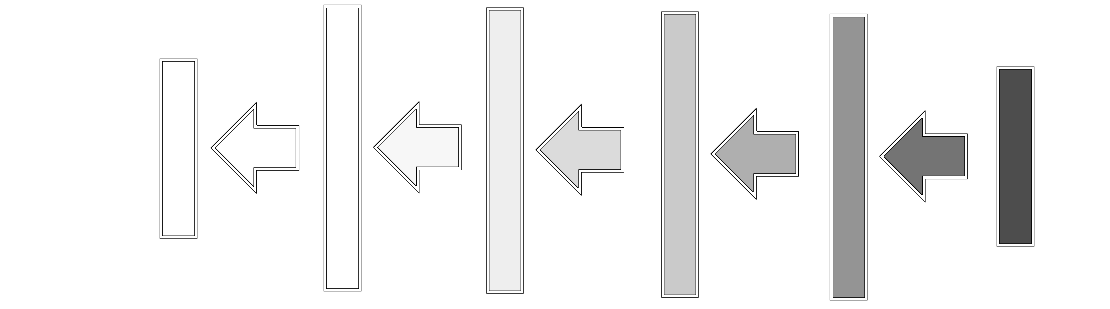
\includegraphics[width=0.7\linewidth]{images/4_vanishing_gradient}
\caption[]{Der \textit{Vanishing Gradient}-Effekt beschreibt bei der Rückpropagierung das abklingende Fehlersignal von Output- hin zu Input-Layer}
\label{fig:4_vanishing_gradient}
\end{figure}

Deutlich wird der Effekt bei der Betrachtung der Formel \ref{eq:vanishgrad1} für das zurück propagierte Fehlersignal $\delta_{message}^l$ im Layer $l$, in der aus Kapitel  \ref{ch:cnn_back} bekannten $\delta_{message}$-Notation.
\begin{equation}
\label{eq:vanishgrad1} 
\delta_{message}^{l} = (W^{l})^T (\delta_{message}^{l+1} \circ \phi'(z^l))
\end{equation}
Setzt man klassische Aktivierungsfunktionen wie $sig(\cdot)$ oder $tanh(\cdot)$ ein (siehe Kapitel \ref{ch:aktivierungsfunktonen}), gilt $\phi'(z^l) <= 1 $. Dies führt zwangsläufig zu einem abklingenden Fehlersignal (\textit{Vanishing Gradient}). Man könnte argumentieren, dass dies durch ein großes $W^l$, sodass $ (W^{l})^T (\delta_{message}^{l+1} \circ \phi'(z^l)) >= 1$, verhindert werden könnte. Dem ist nicht der Fall, da gleichzeitig $z^l = W^lx^l + b^l$ gilt und damit ein großes $W^l$ unweigerlich zu einem großen $z^l$ und damit zu einer kleineren Ableitung der Aktivierungsfunktion, welche ihr Maximum bei $0$ besitzt, führt. Ist zusätzlich zu einem großen $W^l$ der Schwellwert $b^l$ negativ, sodass $z^l \approx 0$, führt dies ebenso nicht zum Verschwinden des Effekts sondern zu einem, nicht weniger ungünstigen, \textit{Exploding Gradient}-Effekt \cite[vgl.][Kapitel 5]{Nielsen2015}). Selbst im linearen Fall ohne Aktivierungsfunktion tritt dieser Effekt auf, wenn die Gewichte jedes Neurons nicht die Norm $\|w\| \approx 1 $ besitzen.
 
Eine normalisierter Initialisierung der Gewichte wirkt diesem Effekt entgegen (vgl. \cite{Glorot2010}). Allerdings scheint erst die Verwendung der neuartigen ReLu-Aktivierungsfunktion (vgl. Kapitel \ref{ch:aktivierungsfunktonen}) den Effekt gänzlich zu unterdrücken und führt darüber hinaus zu oftmals er\-wünsch\-ten, dünnbesetzten (\textit{sparse}) Aktivierungen (vgl. \cite{Glorot2011}). Der Nachteil von ReLu-Neuronen ist allerdings, dass diese bei zu großen Lernraten und damit zu großen Änderungen der Gewichte unwiderruflich sterben (\textit{Dying ReLu}) und somit Teile des Netzes auslöschen können (vgl. \cite{Maas2013}).   


\begin{equation} 
	f(x) =  max(0,x) 
\end{equation}


\begin{figure}
\centering
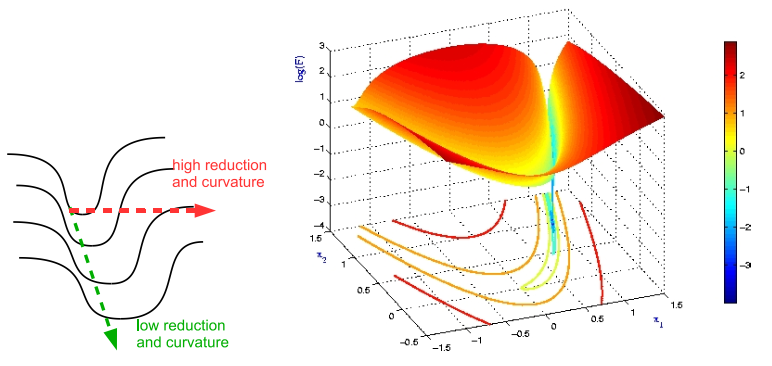
\includegraphics[width=0.5\linewidth]{images/4_pathological_curvature}
\caption[]{Pathological Curvature in der Rosenbrock-Funktion: $f(x,y = (1-x)^2 + 100(y -x^2)^2$ (vgl. \cite{Martens2010})}
\label{fig:4_pathological_curvature}
\end{figure}

Viele der in diesem Kapitel vorgestellten Methoden zielen auf den  \textit{Vanishing Gradient}-Effekt ab, welcher für viele Probleme im Deep-Learning verantwortlich ist. Darüber hinaus zeigt \cite{Martens2010} empirisch, dass die Schwierigkeiten im Deep-Learning auch auf eine ungünstige Fehlerlandschaft (\textit{Pathological Curvature}) zurückzuführen sind. Eine solche ist in Form der Rosenbrock-Funktion in Abbildung \ref{fig:4_pathological_curvature} dargestellt. 

Neben den benannten Problemen hinsichtlich der Fehlerfunktion, führt \textit{Overfitting} häufig ebenso zu schlechten Ergebnissen und entsprechende Regularisierungsmethoden werden benötigt.

\section{Vorverarbeitung}
Der Bereich Vorverarbeitung steht nicht unmittelbar in Zusammenhang mit Deep Learning, wird jedoch zwecks der Vollständigkeit, besonders in Verbindung zu CNNs, vorgestellt.
\cite{Becker1991} stellte bereits Anfang der 1990er Jahre fest, dass durch Dekorrelation der Trainingsdaten MLPs effizienter trainiert werden können. 
\cite{LeCun1998b} fassen die klassische Vorverarbeitung in linearen MLPs wie folgt zusammen:
\begin{itemize}
\item Mittelwertfreie Trainingsdaten verhindern eine steile Fehlerlandschaft. 
\item Die Normalisierung der Varianz unterschiedlicher Merkmale verhindert deren unterschiedliche Gewichtung.
\item Die Dekorrelation der Trainingsdaten führt zwar zu einer diagonalen Hesse-Matrix, allerdings zeigt der Gradient nicht in Richtung Minimum. Dies muss durch dedizierte Lernraten, entsprechend den Kehrwerten der Eigenwerte pro Gewicht, korrigiert werden.
\item Das Whitening der Daten führt zu einer kreisförmigen Fehlerlandschaft mit korrektem Gradienten.
\end{itemize}
Diese Hinweise gelten nur für lineare MLPs und somit quadratische Fehlerlandschaften. Die Fehlerlandschaft der hier verwendeten nicht-linearen MLPs kann jedoch lokal quadratisch approximiert werden (vgl. \cite{Hinton2015}).

Die genannten Techniken können allerdings nicht unmittelbar auf CNNs übertragen werden, da diese versuchen lokale Korrelationen an verschiedenen Orten im Eingaberaum zu extrahieren und die Dekorrelation hochdimensionaler Daten in großer Anzahl sehr rechenintensiv ist.
So zeigt sich bei der Verwendung von CNNs, dass die erfolgreichsten Architekturen lediglich den Mittelwert über die gesamten Trainingsdaten berechnen und diesen von jedem Pixel subtrahieren (vgl. \cite{Krizhevsky2012} und \cite{Simonyan2014}).
\cite{Kaparthy2014} kommen zu einem ähnlichen Schluss und beschreiben für CNNs lediglich die Zentrierung der Daten mittels globalen Mittelwert, alternativ pro Farbkanal oder Pixel, als nötige Vorverarbeitung. 

Teilweise werden für CNNs dennoch zwei weitere Techniken als Praxis beschrieben (vgl. \cite{Andrade2014} und \cite{Goodfellow_maxout_2013}) und deshalb im Folgenden kurz eingeführt.

\subsection{Kontrastnormalisierung}
Das Ziel der Kontrastnormalisierung ist es, unterschiedliche Trainingsbeispiele desselben Objekts in einen ähnlichen Kontrastbereich zu transformieren und so Helligkeitsunterschiede zu kompensieren (vgl. \cite{Zeiler2013b}). 

Die globale Kontrastnormalisierung (GCN) bearbeitet jedes Trainingsbeispiel einzeln und berechnet den Mittelwert und die Varianz über alle Merkmale beziehungsweise Pixel. Im Anschluss wird der Mittelwert subtrahiert und durch die Varianz geteilt \cite[vgl.][]{Sermanet2012}. 
Neben der GCN wird häufig auch die lokale Kontrastnormalisierung (LCN) angewandt. Diese nimmt pro Trainingsbeispiel als Eingabe jeweils nur kleine Umgebungen $k_h \times k_w$ und berechnet die Kontrastnormalisierung für diese Bereiche einzeln \cite[vgl.][]{Jarrett2009}.

\cite{Zeiler2013b} verwenden für Farbbilder den RGB-Raum und normalisieren jeden Kanal einzeln. Dies kann jedoch zu einer Verschiebung des Farbtons führen. Soll dies vermieden werden, wird für Farbbilder entweder der HSV-Raum vorgeschlagen, in welchen nur die Intensität $V$ normalisiert wird \cite[vgl.][S. 56]{Pink2011}. Oder es wird der YUV-Farbraum verwendet und die Normalisierung lediglich auf den Y-Kanal angewandt \cite[vgl.][]{Sermanet2012}.


\subsection{ZCA-Whitening}
Der Begriff \textit{Zero Component Analysis} (ZCA) beschreibt ein der \textit{Principle Component Analysis} (PCA) sehr ähnliches Verfahren (vgl. hierzu und im Folgenden \cite{Krizhevsky2009}). Es zielt darauf ab, die Eingangsdaten so zu dekorrelieren, sodass die Transformation so nahe wie möglich am Original ist. 

\begin{figure}
\centering
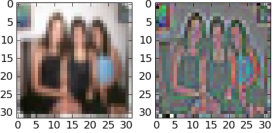
\includegraphics[width=0.5\linewidth]{images/4_ZCA}
\caption[]{Originales Bild (links) und ZCA-transformiertes Bild (rechts) (siehe. \cite{Krizhevsky2009})}
\label{fig:4_ZCA}
\end{figure}

Die Transformationsmatrix $W_{ZCA}$ ist in Gleichung \ref{eq:ZCA} angegeben, wobei die Kovarianzmatrix $C = X^TX$ ist. Der einzige Unterschied zum PCA-Whitening liegt darin, dass eine weitere Rotation zurück in den Bildraum durchgeführt wird. Dies ist möglich, da das Whitening der Daten auch nach einer Rotation mit einer orthogonalen Matrix erhalten bleibt.

\begin{equation}
\label{eq:ZCA} 
W_{ZCA} = C^{-\frac{1}{2}} = P(D+\epsilon)^{-\frac{1}{2}}P^T = PW_{PCA}
\end{equation}

Abbildung \ref{fig:4_ZCA} zeigt die Transformation für ein Beispiel.


\section{Initialisierung}
Die Initialisierung eines neuronalen Netzes ist äußerst wichtig, da die Gewichte ungleich Null sein müssen (\textit{Breaking the Symmetry}). Ansonsten berechnen alle Neuronen die gleiche Ausgabe und es ergeben sich somit die gleichen partiellen Ableitungen \cite[vgl.][S. 201]{Rojas1996}.
\cite{LeCun1989} initialisieren die Gewichte beispielsweise zufällig zwischen $-\frac{2.4}{fan_{in}}$ und $\frac{2.4}{fan_{in}}$, wobei $fan_{in}$ der Anzahl Eingangsneuronen entspricht. Das hat zum Ziel die Nichtlinearität mit Werten um Null zu versorgen und damit nicht zu sättigen (\textit{Vanishing Gradient}).
Das erfolgreiche Netz von \cite{Krizhevsky2012} verwendet beispielsweise die Standard-Initialisierung, eine einfache Normalverteilung mit $W \sim \mathcal{N} (0,0.01)$. Dies ist möglich, da als Aktivierungsfunktionen ReLu-Funktionen verwendet werden, welche nicht sättigen können. 

Daneben existieren im Deep Learning heute zwei Arten zur Initialisierung, welche im Folgenden aufgeführt sind. 

\subsection{Normalisierte Fehlerpropagierung}
\begin{figure}
\centering
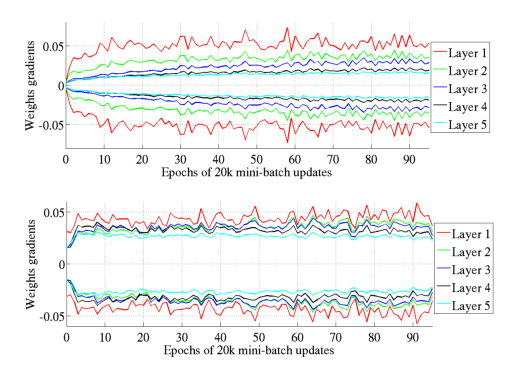
\includegraphics[width=0.7\linewidth]{images/4_xavier_init}
\caption[]{Vergleich der Varianz der Gradienten im Laufe des Trainings (Standard-Initialisierung (oben) und Xavier-Initialisierung (unten)): \textit{Layer 1} entspricht dem Output-Layer mit der größten Varianz im Gradient (siehe \cite{Glorot2010})}
\label{fig:4_xavier_init}
\end{figure}
Stellvertretend für eine derartige Initialisierung der Gewichte, sodass die Varianz des Signals sowohl bei der Berechnung der Ausgabe (\textit{Forward Pass}), als auch bei der Rückpropagierung des Fehlers (\textit{Backward Pass}) gleich groß bleibt  \cite[vgl. z.B.][S. 199 ff.]{Rojas1996}, steht heute die sogenannte \textit{Xavier-Initialization}. Dies führt dazu, dass die Varianz im Gradienten in jeder Schicht in etwa gleich groß ist, was aus Abbildung \ref{fig:4_xavier_init} zu entnehmen ist (vgl. hierzu und im Folgenden \cite{Glorot2010}).
Die \textit{Xavier-Initialization} kombiniert beide Aspekte und initialisiert die Gewichte in der Art, dass die Varianz des Signals von Schicht zu Schicht sowohl im \textit{Forward Pass} als auch im \textit{Backward Pass} erhalten bleibt. Dies wird durch Formel \ref{eq:xavier} erreicht, was letztlich der Anwendung der Varianz-Formel für Gleichverteilung mit $Var(W) = \frac{2}{fan_{in}  + fan_{out}}$ entspricht.

\begin{equation}
\label{eq:xavier} 
W \sim \mathcal{U} [-\frac{\sqrt{6}}{\sqrt{fan_{in}  + fan_{out}}}, \frac{\sqrt{6}}{\sqrt{fan_{in}  + fan_{out}}}]
\end{equation}

Für den Fall, dass ReLu-Funktionen eingesetzt werden, verallgemeinern \cite{He2015} diese Formel insofern, dass eine lineare Approximation um Null für diese und davon abgeleitete Aktivierungsfunktionen nicht mehr gültig ist. Formel \ref{eq:xavier2} entspricht der Verallgemeinerung für Funktionen dieser Art. 

\begin{equation}
\label{eq:xavier2} 
W \sim \mathcal{N} (0,\sqrt{\frac{2}{fan_{out}}})
\end{equation}

Mit der Xavier-Initialisierung werden in Folge häufig bessere Ergebnisse erreicht, als mit der Standard-Initialisierung (\textit{Random Initialization}) in Verbindung mit Informationen über die Krümmung (Approximation der Hesse-Matrix - siehe. Kapitel \ref{ch:2norder}) (vgl. \cite{Chapelle11} und \cite{Glorot2010}).
Für Convolutional Neural Networks berechnen sich \textit{$fan_{in}$} und \textit{$fan_{out}$} durch Multiplikation der Filtergröße mit der Anzahl \textit{Input-Maps} respektive \textit{Feature-Maps} $c$: $k_w \cdot k_h \cdot c$ \cite[vgl.][]{He2015}.


\subsection{Unüberwachtes Vortraining}
Dieses Kapitel weicht die in Kapitel \ref{ch:Einleitung} gemachte Einschränkung auf das klassische überwachte, neuronale Lernmodell insofern auf, als dass ein un\-über\-wach\-tes Lernverfahren vorgestellt wird. Dieses Vorgehen dient jedoch zum einen dem höheren Ziel, das überwachte Verfahren durch eine bessere Initialisierung der Gewichte besser zu konditionieren und in der Performanz zu verbessern. Zum anderen wird sich zeigen, dass es sich bei genauerer Betrachtung nicht um ein klassisches un\-über\-wach\-tes Lernverfahren handelt: Es wird lediglich ein un\-über\-wach\-tes Problem als überwachtes Problem angesehen. 
Dies lässt sich am einfachen Beispiel eines nichtlinearen Autoencoders verdeutlichen \cite[vgl. hierzu und im Folgenden][]{Masci2011}. Der Encoder in Formel \ref{eq:autoenc1} nimmt als Eingabe einen Vektor $x$ und berechnet einen Code $h$.
  
\begin{equation}
\label{eq:autoenc1} 
h = \phi(Wx + b)
\end{equation}

Dieser Code wird im zweiten Schritt durch den Decoder in Formel \ref{eq:autoenc2} dekodiert und so die Ausgabe berechnet. Das Ziel des Autoencoders ist es den Fehler zwischen Eingabe und Rekonstruktion, wie z.B. $MSE = \mathbb{E} [ (x - y)^2 ]$, durch Anpassen der Gewichte $ \theta={W,b} $, wobei $W' = W^T$ (\textit{Tied Weights}), zu minimieren.
 
\begin{equation}
\label{eq:autoenc2} 
y = \phi(W'h + b')
\end{equation}

Der Autoencoder prädiziert folglich die Eingabe selbst und lernt die sogenannte Identität (\textit{Identity Mapping}).
Die Ideen von \cite{Hinton2006}, die gleichzeitig auch den Beginn der Renaissance von Deep Learning darstellen, beschreiben ein Verfahren große Netzwerke mit vielen Schichten schichtweise \textit{greedy} mit beschränkten Boltzmann Maschinen (RBMs) zu trainieren (vgl. \cite{Bengio2007}). Das bedeutet, dass jede Schicht als Eingabe die Ausgabe der vorherigen Schicht erhält und versucht, diese wiederum zu prädizieren (vgl. \cite{Ranzato2006}). Dies wirkt ähnlich wie ein Regularisierer und initialisiert die Gewichte hinsichtlich der Optimierung und Generalisierung in einer besseren Ausgangssituation \cite[vgl.][]{Erhan2010}. Hiervon profitieren besonders große MLPs, welche bis dato aufgrund des \textit{Vanishing-Gradient}-Effekts als schwer zu trainieren galten. 

Eine wichtige Weiterentwicklung des Konzepts sind sogenannte \textit{Denoising Autoencoder} (DAs) beziehungsweise \textit{Stacked Denoising Autoencoder} (SDA), welche versuchen die Eingabe $ x $ ausgehend von einer korrumpierten Version $ \hat{x} $ zu prädizieren. Dies erlaubt das Erlernen robuster Merkmale und kann als diskriminative Alternative zum generativen stochastischen RBM-Modell gesehen werden (vgl. \cite{Vincent2008}). 

Convolutional Neural Networks wie das \textit{LeNet 5} von \cite{LeCun1998} können aufgrund ihrer besonderen Struktur dennoch trainiert werden. Trotzdem ist es auch bei CNNs schwierig die ersten Schichten zu trainieren, da die hinteren Schichten generell schneller unscheinbares \textit{Overfitting} mit entsprechend kleinem Gradienten aufweisen (vgl. \cite{Erhan2010}). Der erste Versuch un\-über\-wach\-tes Vortraining auf CNNs anzuwenden stammt von \cite{Ranzato2006}. Hier wird die erste Schicht eines veränderten \textit{LeNet 5} mittels Vortraining initialisiert, was den Fehler auf dem MNIST-Datensatz\footnote{Der MNIST-Datensatz handgeschriebener Ziffern besteht aus 60,000 Trainingsbeispielen und 10,000 Testbeispielen. Es stellt eine Untermenge des größeren NIST-Datensatzes dar. Die Bilder sind $28 \times 28$ und die Ziffern zentriert (\url{http://yann.lecun.com/exdb/mnist/} (26.08.2015)).} von $0.7 \%$ auf $0.6 \%$ verringert. Das Vortraining der $5 \times 5$-Filter geschieht mit zufällig gewählten $5 \times 5$-Bildausschnitten auf der Basis von RBMs.


\subsubsection{Convolutional Autoencoder}
\label{ch:autoenc}
Es existieren verschiedenste Architekturvorschläge für Autoencoder und RBMs zum Vortraining von CNNs. Die Grundlage hierfür ist meist die Extraktion den Filter entsprechend großer Bildausschnitte und das Trainieren gewohnter Modelle (vgl. \cite{Desjardins2008}, \cite{Ranzato2007} oder \cite{Lee2009}).  
Im Folgenden wird der Convolutional Autoencoder von \cite{Masci2011} vorgestellt, da dieser auf Faltungen basiert und, wie Abbildung \ref{fig:4_mascii} zeigt, die gewünschten translationsinvarianten Filter erzeugt. Die vorgestellte Variante verbessert im Rahmen der Experimente von \cite{Masci2011} den Testfehler auf dem MNIST-Datensatz von $0.79 \%$ auf $0.71 \%$.

\begin{figure}
\centering
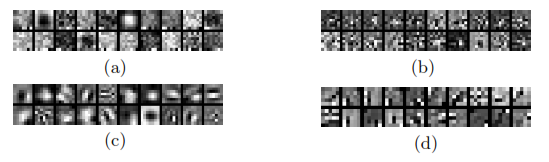
\includegraphics[width=0.7\linewidth]{images/4_mascii}
\caption[]{Filter der ersten Schicht eines Convolutional Autoencoders (a) Kein Max-Pooling, 0 \% Rauschen, (b) Kein Max-Pooling, 50 \% Rauschen, (c) Max-Pooling $2 \times 2$, (d) Max-Pooling $2 \times 2$, 30 \% Rauschen (siehe \cite{Masci2011})}
\label{fig:4_mascii}
\end{figure}

Die Architektur des vorgestellten Convolutional Autoencoders besteht aus einem Convolution-Layer sowie einem nachgeschalteten Pooling-Layer. Das bedeutet, dass sich der gesamte Autoencoder letztendlich aus zwei hintereinander ausgeführte Layern dieser Art zusammensetzt.

Gleichung \ref{eq:cautoenc1} zeigt die Berechnung des Codes $h_i$ der $i$-ten \textit{Feature-Map}. Dieser wird wie in gewöhnlichen CNNs durch Faltung mit Randbehandlung \textit{valid} berechnet. 

\begin{equation}
\label{eq:cautoenc1} 
h_i = \phi(\sum_{j=0}^{m}  x_{j} \ast W_{ij} + b_i)
\end{equation}

Der Decoder berechnet die Funktion \ref{eq:cautoenc2}, wobei ähnlich dem \textit{Backward Pass} im Backpropagation die Filtermaske über beide Seiten geflippt beziehungsweise um $180^\circ$ gedreht und die Randbehandlung \textit{full} verwendet wird. Die Dekodierung ist beeinflusst von gewöhnlichen Autoencodern mit \textit{Tied Weights}, bei denen als Dekodierungsfunktion ebenfalls die transponierte Gewichtsmatrix des \textit{Forward Pass} verwendet wird.

\begin{equation}
\label{eq:cautoenc2} 
y_j = \phi(\sum_{i=0}^{n} h_{i} \ast rot180(W_{ij}) + c_j)
\end{equation}

Der Gradient für den Autoencoder berechnet sich mit Formel \ref{eq:cautoenc3}. Diese setzt sich, wie der Autoencoder, aus zwei Teilen zusammen. Der erste Teil wird für den Encoder, der zweite für den Decoder benötigt. Im Unterschied zur Berechnung des Gradienten beim CNN wird anstatt $\delta y$ der Code $h$ der Flip-Operation unterzogen. Dies tritt auf, da der \textit{Backward Pass} dem eigentlichen \textit{Forward Pass} entspricht.\footnote{Im Unterschied zur von \cite{Masci2011} beschriebenen Berechnung wird in Konsequenz auch auf die Flip-Operation von $\delta h$ nicht verzichtet und der Gradient am Ende gesamtheitlich geflippt. Der Gradient für den Encoder wird damit äquivalent zu dem in einem CNN berechnet. In Kapitel \ref{ch:debug} wird die Richtigkeit dieser Änderung überprüft.}
Eine zusätzliche Besonderheit besteht in Zusammenhang mit der Randbehandlung \textit{valid}. Um den Code $rot180(h)$ mit dem räumlich größeren $\delta y$ der Ausgabe zu falten, muss dieser doppelt mit Nullen erweitert werden (Padding). Zum einen um die gleiche Größe wie die Ausgabe zu erhalten und zum anderen um die Faltung zu ermöglichen.

\begin{equation}
\label{eq:cautoenc3} 
\frac{\partial J(W,b,c)}{\partial W_{ij}^l} = \frac{1}{M} \sum_{m=1}^{M} rot180(x_{mj}^l \ast  rot180(\delta h_{mi}^l) + rot180(h_{mi}^l) \ast \delta y_{mj}^l)   
\end{equation}

Analog zum bekannten Convolution-Layer wird über alle Trainingsbeispiele $M$ gemittelt und die beiden Schwellwerte $b$ und $c$ berechnen sich aus der Summe der zugehörigen Deltas $\delta y$ und $\delta h$, wie in Gleichung \ref{eq:cautoenc4} und \ref{eq:cautoenc5} dargestellt ist.

\begin{equation}
\label{eq:cautoenc4} 
\frac{\partial J(W,b,c)}{\partial b_{i}^l} = \frac{1}{M} \sum_{m=1}^{M} \sum_{u=0}^{k_w} \sum_{v=0}^{k_w} \delta h_{miuv}^{l} 
\end{equation}


\begin{equation}
\label{eq:cautoenc5} 
\frac{\partial J(W,b,c)}{\partial c_{j}^l} = \frac{1}{M} \sum_{m=1}^{M} \sum_{u=0}^{k_w} \sum_{v=0}^{k_w} \delta y_{miuv}^{l} 
\end{equation}


Weiterentwicklungen wie die \textit{Tiled CNNs} versuchen weitere Invarianzen, wie beispielsweise die Rotationsinvarianz, zu lernen (vgl. \cite{Quoc2010}).
Einer der größten Autoencoder, der \textit{Google Autoencoder}, bedient sich ebenfalls der lokalen rezeptiven Felder, verzichtet allerdings auf \textit{Parameter Sharing}, um verschiedene Invarianzen zu lernen (vgl. \cite{LeRanzato2012}). Eine Schicht dieser Architektur ist in Abbildung \ref{fig:4_ranzato} abgebildet.

\begin{figure}
\centering
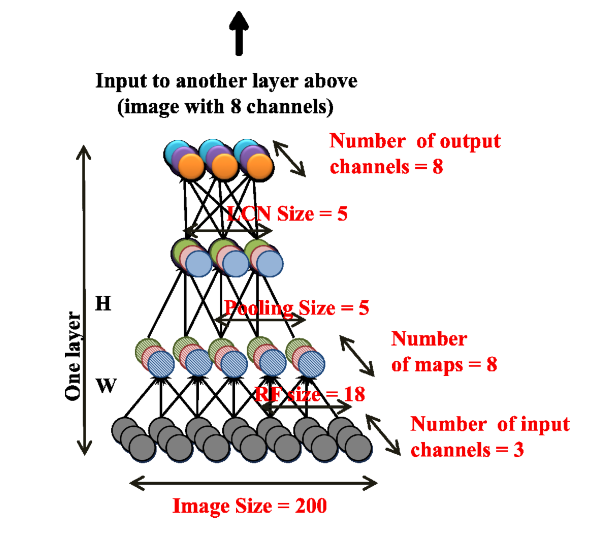
\includegraphics[width=0.5\linewidth]{images/4_ranzato}
\caption[]{Autoencoder mit lokalen rezeptiven Feldern aber ohne \textit{Parameter Sharing} (siehe \cite{LeRanzato2012})}
\label{fig:4_ranzato}
\end{figure}


Auch wenn das Verwenden von un\-über\-wach\-tem Vortraining für die ersten Schichten eines CNNs passend erscheinen mag, führt es nicht zu einer solchen Verbesserung der Ergebnisse wie bei tiefen MLPs (DNNs) (vgl. \cite{Hamid2013}). 
Durch die Entwicklung neuer Aktivierungsfunktionen wie ReLu und raffinierter Initialisierung rückt das Thema somit in solche Bereiche, in denen wenig gelabelte Trainingsdaten zur Verfügung stehen, um das CNN vollständig überwacht zu trainieren (vgl. \cite{Masci2011} und \cite{LeRanzato2012}). Darüber hinaus können auch verbesserte Optimierungsverfahren das un\-über\-wach\-te Vortraining hinsichtlich einer besseren Initialisierung ersetzen (vgl. \cite{Martens2010} und \cite{Sutskever2013}). 

Eine neue Herangehensweise ist es, bereits trainierte CNNs für andere Probleme zu übernehmen, was als sogenanntes Transferlernen bezeichnet wird (vgl. \cite{Wagner2013}). So liefert zum Beispiel die 7. Schicht des \textit{AlexNet} von \cite{Krizhevsky2012} bereits sehr gute Bildbeschreibungen (vgl. \cite{Bell2015} und \cite{Kaparthy2014}).


\section{Gradientenabstieg}
\label{ch:gradient}
\begin{figure}
\centering
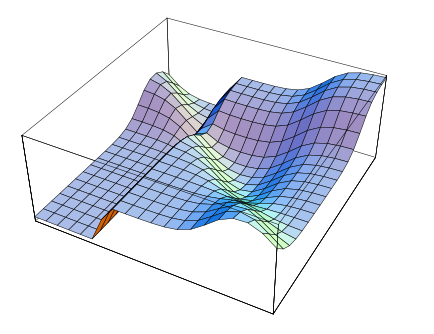
\includegraphics[width=0.5\linewidth]{images/4_Gradient2}
\caption[]{Fehlerfunktion beziehungsweise Zielfunktion im Gewichtsraum mit lokalem Minimum \cite[siehe][S. 155]{Rojas1996} }%\cite[siehe][Kap. 5, S. 17]{Duda2001}}
\label{fig:4_Gradient}
\end{figure}
Dieses Kapitel behandelt verschiedene Methoden zur Verbesserung des Gradientenabstiegs. Diese können das Training erheblich beschleunigen, da es sich im Allgemeinen im Deep Learning um nicht-konvexe Fehlerlandschaften wie in Abbildung \ref{fig:4_Gradient} handelt.

Die Grundlage für das effiziente Lernen mit vielen Trainingsdaten ist der sogenannte stochastische Gradientenabstieg (SGD) (vgl. hierzu und im Folgenden \cite{Bottou1998}). Hierbei geht es um die Frage, was die erwartete durchschnittliche Richtung des Gradienten ist. Durch die Einführung des MSE-Fehlermaßes ist der Ansatz des SGD bereits gegeben. So entspricht die MSE-Fehlerfunktion dem Erwartungswert der einzelnen Fehlerquadrate. Wie in Gleichung \ref{eq:sgd_mse} zu sehen ist, entspricht analog dazu der Erwartungswert der einzelnen Gradienten dem Gradient der Fehlerfunktion.

\begin{equation}
\label{eq:sgd_mse} 
\nabla J(W,b) =  \mathbb{E}[\nabla (f(x_i) - y_i)^2] = \frac{1}{N}\sum_{i}^{N} \nabla (f(x_i) - y_i)^2
\end{equation}

Für eine allgemeine Fehlerfunktion $e(x)$ gilt: Nimmt man an Stelle der gesamten Trainingsmenge $N$ (Batch) einzelne Trainingsbeispiele $i$ (Online) oder eine Teilmenge $M$ (Averaged SGD), so ergibt sich Formel \ref{eq:sgd} für den Gradientenabstieg mit Lernrate beziehungsweise Schrittweite $\eta$. Der Gradient zeigt somit in Richtung des Durchschnitts und damit in Richtung des Erwartungswerts. 

Neben einer effizienteren Berechnung des Gradientenabstiegs, liefert SGD eine Zufallskomponente (\textit{Randomization}) \cite[vgl. hierzu und im Folgenden][]{Bengio2012}. Diese kann zu beschleunigter Konvergenz führen, da durch variierende (\textit{noisy}) Gewichtsupdates ein größeres Gebiet untersucht werden kann. Außerdem erlaubt SGD Training ohne unmittelbarem Zugriff auf die gesamte Trainingsmenge. Üblicherweise werden die für die Berechnung entnommenen Teilmengen als \textit{Mini-Batch} bezeichnet.

\begin{equation}
\label{eq:sgd} 
W_{t+1} = W_t - \eta \frac{1}{M} \sum_{i=1}^{M} \nabla e(x_i)
\end{equation}

SGD bildet die Grundlage für viele Erweiterungen und stellt so die erste Optimierung des Gradientenabstiegs dar. 
Um die Formeln zu vereinfachen, wird im Folgenden auf die sonst obligatorische Mittelung des Gradienten verzichtet. An den entsprechenden Stellen wird darauf hingewiesen, ob es sich um die Erweiterung für den Online-/Mini-Batch-Modus oder um den klassischen Batch-Modus, welcher für Deep Learning in Verbindung mit vielen Trainingsdaten unpraktikabel ist, handelt. 

\subsubsection{Lernrate und Mini-Batch-Größe}

Wird der klassische Gradientenabstieg ohne Optimierungen verwendet, ist es besonders wichtig $\eta$ richtig zu wählen. Aufgrund des \textit{Vanishing Gradient}-Effekts sollte die Lernrate in den letzten Schichten kleiner gewählt werden. Außerdem ist darauf zu achten, dass die Lernrate durch \textit{Parameter Sharing} proportional zur Wurzel der Verbindungen ist, die sich ein Gewicht teilen. Letzteres ist gerade bei CNNs zu beachten, um eine unnötig schlechte Konditionierung der Fehlerlandschaft zu vermeiden (vgl. \cite{LeCun1998b}).

Die Bestimmung der Mini-Batch-Größe $M$ erlaubt es zwischen Online- und Batch-Training zu interpolieren. Dies ist wichtig, da die richtige Wahl der Größe von den Trainingsdaten abhängt und nicht allgemein vorhergesagt werden kann. So kann beispielsweise Online-Training in vielen Situationen schneller sein als Batch-Training  \cite[vgl.][]{Wilson2003}. Als Stellgröße kann der Grad an Redundanz in den Trainingsdaten dienen. Mit steigender Redundanz sollten die Batches entsprechend kleiner gewählt werden, um nicht unnötig Rechenzeit zu verbrauchen. \cite{Bengio2012} nennt $M = 32$ einen guten Standardwert.

\subsection{Momentum}
Eine der ersten erfolgreichen Erweiterungen für iterative Verfahren ist die sogenannte Momentum Methode von \cite{Polyak1964}.
Die Momentum-Methode ist durch die Physik motiviert, dadurch dass dem Gradienten eine potentielle Energie zugewiesen wird. Dies erlaubt es in gleichbleibender Richtung des Gradienten Geschwindigkeit aufzunehmen. Dies führt letztendlich dazu, dass in flachen Regionen der Fehlerlandschaft größere und in unwegsamen Bereichen kleinere Schrittweiten effektiv ausgeführt werden (vgl. \cite{LeCun1998b}).
Dies wird durch das Hinzufügen eines weiteren Terms in das Gewichtsupdate erzielt. Wie Formeln \ref{eq:momentum} und \ref{eq:momentum1} zeigen, bildet die Momentum-Methode einen gewichteten Durchschnitt der vergangenen Gradienten der Gewichte. 
 
\begin{equation}
\label{eq:momentum} 
\Delta W_t = \mu \Delta W_{t-1} - \eta \nabla J(W_t,b_t)
\end{equation} 
 
\begin{equation}
\label{eq:momentum1} 
W_{t+1} = W_t + \Delta W_t
\end{equation}
Typische Werte für die Momentum-Rate $\mu$ sind Werte größer $0.9$. Diese sind allerdings abhängig vom Lernproblem und können nicht allgemein formuliert werden (vgl. \cite{Kaparthy2014}). Die Momentum-Methode ist eine sehr einfache Optimierung für SGD und findet in erfolgreichen Netzen häufig Anwendung (vgl. \cite{Krizhevsky2012}).

\subsubsection{Nesterov-Methode}
Die Nesterov-Methode (NAG) ist eine verbesserte Momentum-Methode, die von \cite{Nesterov1983} beeinflusst ist \cite[vgl. hierzu und im Folgenden][]{Sutskever2013b}. Diese Methode führt zunächst den über die vergangenen Perioden gewichteten Momentum-Term aus und berechnet dann den Gradient an dieser Stelle. Die Methode fungiert somit als eine Art Ausblick auf die zukünftige Fehlerlandschaft. Der eigentliche Gradient ergibt sich schließlich aus Ausblick und Korrektur, wie Abbildung \ref{fig:4_nesterov} zeigt.
\begin{figure}
\centering
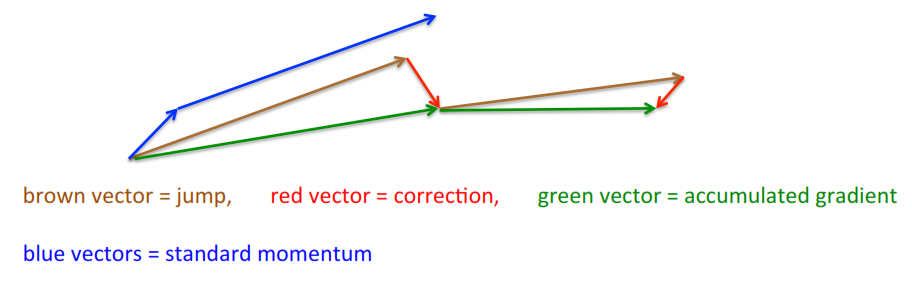
\includegraphics[width=0.7\linewidth]{images/4_nesterov}
\caption[]{Das effektivere Nesterov-Momentum korrigiert Fehler im Nachhinein\cite[siehe][]{Hinton2015} }%\cite[siehe][Kap. 5, S. 17]{Duda2001}}
\label{fig:4_nesterov}
\end{figure}

Da diese Ausführung die Reihenfolge des üblichen Trainings beeinflussen würde, wird die Methode derart umgeschrieben, dass die aktuellen Gewichte immer dem Ausblick entsprechen. Daraus ergeben sich die Regeln \ref{eq:nesterov1} und \ref{eq:nesterov2} für die Aktualisierung der Gewichte (vgl. \cite{Kaparthy2014}).


\begin{equation}
\label{eq:nesterov1} 
\Delta W_t = \mu \Delta W_{t-1} - \eta  \nabla J(W_t,b_t)
\end{equation}
\begin{equation}
\label{eq:nesterov2} 
W_{t+1} = W_t + (-\mu \Delta W_{t-1} ) + (1 + \mu) \Delta W_t
\end{equation}

Die beschriebene Methode ist nach \cite{Sutskever2013} robuster hinsichtlich der Momentum-Rate und lässt höhere Raten zwischen $0.9$ und $0.99$ zu. 

\subsection{Adaptive Lernrate}
\label{ch:2norder}
Ein allgemeines Problem in Verbindung von Gradientenabstieg und dem Training im Deep Learning ist der \textit{Vanishing Gradient}-Effekt nach \cite{Hochreiter1991}. Ein Algorithmus der direkt auf diesen Effekt abzielt, ist der sogenannte Resilient Propagation, auch Rprop genannt (vgl. \cite{Riedmiller1992} und \cite{Igel2000}). Rprop weist jedem Gewicht eine eigene Lernrate zu und verzichtet verwendet nur das Vorzeichen des Gradienten. Die grundlegende Arbeitsweise sieht vor, bei gleichbleibendem Vorzeichen der partiellen Ableitung eines Gewichts die zugehörige Lernrate zu erhöhen. Tritt ein Vorzeichenwechsel auf, so liegt es nahe, dass in der Richtung dieser Ableitung eine Senke übersprungen wurde und die Lernrate wird reduziert. Rprop ist nach \cite{Hinton2015} äquivalent zum Gradientenabstieg im Batch-Modus, wenn bei letzterem durch die Länge des Gradient geteilt wird.
Hier liegt ein fundamentales Problem hinsichtlich Deep Learning: Um die Länge des Gradienten korrekt zu schätzen, bedarf es der gesamten Trainingsmenge, was die Verwendung von SGD ausschließt. Somit ist Rprop nur für Batch-Training geeignet (vgl. \cite{Hinton2015}).



Der bekannte Newton-Algorithmus für Optimierung in Gleichung \ref{eq:hessianstep} multipliziert nicht mit einer globalen Lernrate, sondern mit der Inversen der Hesse-Matrix. Unter bestimmten Annahmen, wie etwa einer quadratischen Zielfunktion, erreicht dieser Algorithmus innerhalb eines Schrittes das Minimum, was als Newton-Schritt bezeichnet wird (vgl. \cite{Bottou1998}).

\begin{equation}
\label{eq:hessianstep} 
W_{t+1} = W_t - H_t^{-1} \nabla J(W_t,b_t)
\end{equation}

Die Hesse-Matrix ist im Allgemeinen sehr teuer zu berechnen, da jede partielle Ableitung der $N$ Gewichte nochmals abgeleitet werden müsste. Dies führt auf eine $N \times N $-Matrix, welche in neuronalen Netzen nicht effizient zu berechnen ist und deshalb approximiert werden muss \cite[vgl.][]{LeCun1998b}. 

Algorithmen mit sogenannter adaptiver Lernrate gehen so vor, dass sie lediglich die Diagonale der Hesse-Matrix $diag(H)$ approximieren. Dies führt zu eigenen Lernraten pro Gewicht, welche idealerweise den echten Eigenwerten der Hesse-Matrix entsprechen \cite[vgl.][]{LeCun1998b}. Adaptive Lernraten erlauben es, Schrittweiten in Gegenden schwacher Krümmung zu erhöhen und entsprechend in anderen zu verkürzen. Dieser Mechanismus wirkt damit ebenso unmittelbar dem \textit{Vanishing Gradient}-Effekt entgegen, da kleiner werdende Gradienten zu den ersten Schichten hin skaliert werden \cite[vgl.][]{Martens2010}. 
Problematisch bei der Verwendung der Hesse-Matrix für nicht-konvexe Probleme sind negative Eigenwerte an lokalen Maxima oder gemischt positive und negative Eigenwerte an Sattelpunkten, die zu einer falschen Richtung des Gradienten führen \cite[vgl.][]{Dauphin14}. Aus diesem Grund ist es notwendig, eine Methode mit entsprechender Vorkonditionierung zu verwenden \cite[vgl.][]{Dauphin2015}.


\subsubsection{Stochastischer Levenberg-Marquardt}
Der bekannte stochastische Levenberg-Marquardt-Algorithmus (LMA) von \cite{LeCun1998b} ist ein Algorithmus im Bereich Neuronale Netze und SGD, der versucht die $diag(H)$ zu approximieren. Hierzu sind allerdings zwei weitere Approximationen notwendig. So wird die Gauß-Newton Approximation zur Vermeidung negativer Eigenwerte, wie im klassischen LMA-Algorithmus, angewandt und die $diag(H)$ nur auf einer kleinen Teilmenge der Trainingsdaten (Mini-Batch) berechnet. Darüber hinaus wird die Berechnung nur einmal pro Epoche durchgeführt. Die Kosten entsprechen denen eines normalen \textit{Forward Pass} sowie einem angepassten \textit{Backward Pass}, der zur Rückpropagierung der zweiten Ableitungen dient, und sind somit zu vernachlässigen. 
Neben der Kompensation des \textit{Vanishing-Gradient}-Effekts durch adaptive Lernraten, kompensiert der stochastische LMA den Effekt der schlechten Konditionierung der Fehlerlandschaft durch \textit{Parameter Sharing} \cite[vgl.][]{LeCun1998b}.
Die neue Lernrate pro Gewicht $i$ ergibt sich mit Formel \ref{eq:lma}.

\begin{equation}
\label{eq:lma} 
\eta_{i} = \frac{\eta}{\mu + H_{ii}}
\end{equation}

Wie im klassischen LMA wird ein Dämpfungsfaktor $\mu$ verwendet, um zu verhindern, dass die Schrittweite zu groß wird. Dieser Faktor kann auch als Vorannahme gesehen werden, die angibt, dass sich das Gewicht nicht ändern soll, wenn die Krümmung entsprechend klein wird (vgl. \cite{Martens2010}). Im \textit{LeNet 5} wird $\mu = 0.02$ verwendet.


\subsubsection{Equilibrium SGD}
Eine Verbesserung zum stochastischen LMA ist die von \cite{Dauphin2015} beschriebene Equilibrium-Methode, welche die Matrix $D^{Eq} = \sqrt{diag(H^2)})$ berechnet. Diese Vorkonditionierung bietet einige Vorteile hinsichtlich der Behandlung der genannten indefiniten Hesse-Matrizen, die durch Sattelpunkten innerhalb der Fehlerlandschaft von MLPs auftreten. Darüber hinaus kann diese Methode effizient durch den Zusammenhang in Formel \ref{eq:equi} mit $v \sim \mathcal{N} (0,1)$, beispielsweise mit dem $R\{\cdot\}$-Operator (vgl. \cite{Pearlmutter1994}), berechnet werden. 

\begin{equation}
\label{eq:equi} 
D^{Eq} = diag(H^2) = E[(Hv)^2]
\end{equation}

Im Unterschied zum stochastischen LMA bildet die Equilibrium-Methode, wie Formel \ref{eq:equi1} zeigt, einen  \textit{Root Mean Square}-Durchschnitt (RMS) über die vergangenen Perioden. \cite{Dauphin2015} schlagen eine Neuberechnung von $D^{eq}$ nach jeweils 20 Iterationen und $\mu \in [10^{-4},10^{-6}]$ vor.

\begin{equation}
\label{eq:equi1} 
D^{eq}_{t+1} = \rho D^{eq}_{t} + (1 - \rho) (Hv)^2
\end{equation}

Damit ergibt sich die in Formel \ref{eq:equi2} gezeigte effektive Lernrate, welche ebenfalls einen Dämpfungsfaktor $\mu$ zur Vermeidung großer Schrittweiten beinhaltet.

\begin{equation}
\label{eq:equi2} 
\eta_{i} = \frac{\eta}{\mu + \sqrt{D^{eq}_{ii}}}
\end{equation}

\subsubsection{RMSprop}
Der RMSprop-Algorithmus stammt von \cite{Hinton2015} und kombiniert zwei Ideen. Einerseits die Idee des Rprop nur auf das Vorzeichen des Gradienten zu achten, indem er den \textit{Root Mean Square}-Durchschnitt (RMS) der partiellen Ableitungen über mehrere Zeitschritte berechnet. Andererseits wird das Hauptproblem von AdaGrad der stetig kleiner werdenden effektiven Lernraten dadurch vermieden \cite[vgl.][Kap. 8.4.1, S. 257]{Bengio2015}. Die Formel \ref{eq:rmsprop1} beschreibt die Berechnung des RMS. Die effektive Lernrate berechnet sich mit der Formel \ref{eq:rmsprop2}, wobei ebenfalls ein Dämpfungsfaktor $\mu$ verwendet wird. Der Parameter $\rho$ gibt an mit welcher Rate der exponentiell geglättete Mittelwert abnimmt. \cite{Dauphin2015} schlagen $\mu = 10^{-2}$ und $\rho = 0.9$ als robuste Werte vor.

\begin{equation}
\label{eq:rmsprop1} 
\hat{H}_{t+1} = \rho \hat{H}_{t} + (1 - \rho) \nabla J(W_t,b_t)^2
\end{equation}


\begin{equation}
\label{eq:rmsprop2} 
\eta_{i} = \frac{\eta}{\mu + \sqrt{\hat{H}_{ii}}}
\end{equation}

Eine sehr interessante Eigenschaft von RMSprop ist die Fähigkeit zur Approximation der Equilibrium-Matrix $D^{Eq} = \sqrt{diag(H^2)})$ (vgl. \cite{Dauphin2015}). RMSprop stellt eine sehr effektive und praktische Optimierung dar, welche dazu einfach zu implementieren ist. Dies macht diese derzeit sehr beliebt (vgl. \cite{Bengio2015}).

\subsubsection{AdaDelta}
AdaDelta ist ein von \cite{Zeiler2012} entwickeltes Verfahren, welches ebenfalls das Problem der immer kleiner werdenden Lernrate von AdaGrad adressiert (vgl. \cite{Bengio2015}). Darüber hinaus versucht AdaDelta aus der ersten Ableitung die Krümmung der Funktion (\textit{Second Order Information}) zu berechnen. Der Divisor in Formel \ref{eq:adadelta1} entspricht, bis auf dem unter der Wurzel stehenden $\mu$, dem des RMSprop aus Formel \ref{eq:rmsprop1}. Eine Neuheit stellt der RMS über den Gewichtsupdates $RMS[\Delta x]$, der einen Zeitschritt versetzt berechnet wird und als eine Art Momentum wirkt. Insgesamt schätzt die AdaDelta-Methode die absolute Hesse-Matrix $|diag(H)|$ aus Gradient und Gewichtsupdate \cite[vgl.][]{Zeiler2012}.


\begin{equation}
\label{eq:adadelta1} 
\Delta x_{t} = \frac{\sqrt{\mu + RMS[\Delta x]^2_{t-1} }}{\sqrt{\mu + \hat{H}_{t}}} 
\end{equation}

Die effektive Lernrate ergibt sich aus Formel \ref{eq:adadelta3}.

\begin{equation}
\label{eq:adadelta3} 
 \eta_{i} = \Delta x_i
\end{equation}

Eine Besonderheit von AdaDelta ist, dass gänzlich auf eine globale Lernrate verzichtet und lediglich $\mu$ und $\rho$ als Hyperparameter benötigt werden. Da sich $\mu$ unter der Wurzel befindet ist dieses entsprechend kleiner als bei den vorherigen Methoden. \cite{Zeiler2012} schlägt hierbei Werte bis $\mu = 10^{-8}$ vor. Auch wenn ursprünglich in \cite{Zeiler2012} keine Lernrate beschrieben ist, kann es für manche Szenarios dennoch nützlich sein, zusätzlich eine Lernrate zu implementieren. Beispielweise um diese im Laufe des Trainings zu reduzieren.


\subsection{Hessian Free Optimazation (HF)}
\label{ch:hf}

Algorithmen mit adaptiver Lernrate vernachlässigen, im Sinne der Approximation, alle nicht-diagonalen Werte der Hesse-Matrix. Damit wird ein gewisser Fehler akzeptiert, da diese Werte gerade die Interaktion der Gewichte hinsichtlich der Zielfunktion beschreiben (vgl. hierzu und im Folgenden \cite{Martens2010}). 

Die \textit{Hessian Free Optimazation} (HF) von \cite{Martens2010} versucht, im Gegensatz zu den vorherigen Methoden, nicht den \textit{Vanishing Gradient}-Effekt zu eliminieren oder Plateaus zu überwinden, sondern zielt direkt auf die Optimierung von ungünstigen Fehlerlandschaften (\textit{Pathological Curvature}) ab.
Für eine gegebene Stelle $w_t$ im Gewichtsraum wird ein lokales quadratisches Modell angenommen und dieses mittels Conjugate  Gradient (CG) optimiert. Deshalb kann HF nur im \textit{Batch}-Modus betrieben oder, analog zum stochastischen LMA, mit einer hinreichend großen Teilmenge der Trainingsdaten. Eine Besonderheit dieser Methode ist, dass der gefundene Vektor von CG im letzten Zeitschritt als Initialisierung für den aktuellen Zeitschritt gewählt werden und dadurch Informationen über mehrere Iterationen weitergeben kann.

\cite{Sutskever2013} unterziehen diese Methode einer kritischen Betrachtung und stellen fest, dass sie, aufgrund der Verwendung des linearen CG, keine Methode 2. Ordnung und daher den anderen Methoden nicht allgemein überlegen ist. So zeigen \cite{Sutskever2013}, dass die vorgestellte HF-Methode sehr viele Ähnlichkeiten zum Nesterov-Momentum aufweist und zu diesem unter der Annahme, dass nur ein Schritt im CG-Algorithmus ausgeführt wird, sogar äquivalent ist. Sie kommen zu dem Schluss, dass die interessante Eigenschaft, die Schrittweiten in Bereichen mit geringer Krümmung zu erhöhen und in Bereichen großer Krümmung entsprechend zu verringern, auf beide Methoden HF und NAG zutrifft. Damit sprechen sie der NAG-Methode besonders im Bereich tiefer Netze großes Potenzial zu.
					

\section{Regularisierung und Generalisierung}
Lernprobleme selbst lassen sich beispielsweise mit bayesianischer Inferenz anschaulich beschreiben \cite[vgl. hierzu und im Folgenden][S. 159f]{Mitchell1997}.
\begin{equation}
\label{eq:bayesParam}
P(h|\mathcal{D}) = \frac{P(\mathcal{D}|h)P(h)}{P(\mathcal{D})}
\end{equation}
So beschreibt die Formel \ref{eq:bayesParam} den Zusammenhang zwischen gegebenen Trainingsdaten $\mathcal{D}$ und der Hypothese $h$, welche den zu erlernenden Parametern  $\Theta = \{W,b\} $ entspricht. Sie soll die gegebenen Daten $\mathcal{D}$ möglichst gut abbilden können sowie eine gute Generalisierung für unbekannte Daten leisten. In der bayesianischen Interpretation korrespondieren Regularisierer mit der A-priori Verteilung der Hypothese $h$.

Im Deep Learning existieren verschiedenste Methode der Regularisierung, welche auf eine bessere Generalisierung abzielen \cite[vgl. hierzu und im Folgenden][Kap. 7, S. 196]{Bengio2015}. Manche betreffen die Parameter selbst, andere codieren Expertenwissen oder regulieren die Kapazität von Modellen mit sehr vielen freien Parametern. 
Im Umfeld neuronaler Netze betrifft die Regularisierung von Parametern meist lediglich die Gewichte $W$, der Schwellwert $b$ bleibt unbeachtet (vgl. \cite{Hinton2012} ,\cite{Kaparthy2014} und \cite{Srivastava2014}).
					

\subsection{A-priori Annahmen}

Die A-priori Verteilung der Parameter $\Theta$ gibt an wie wahrscheinlich verschiedene Werte für die einzelnen Parameter sind. Die klassischen Methoden des maschinellen Lernens sowie der Statistik bestrafen die Norm der Parameter (\textit{Parameter Norm Penalty}) und vermeiden so große Werte dieser. Die Norm wird als $\Omega(\Theta)$ definiert und zur Zielfunktion, wie in Gleichung \ref{[eq:reg1]}, gewichtet mit dem Hyperparameter $\alpha$ addiert \cite[vgl.][Kap. 7.2, S. 200]{Bengio2015}. 

\begin{equation}
\label{[eq:reg1]}
\hat{J}(W,b) =  J(W,b) + \alpha \Omega(\Theta)
\end{equation}

Typische Normen sind die $L^1$- und $L^2$-Norm. Abbildung \ref{fig:4_regularizer} stellt die beiden Varianten gegenüber.

\begin{figure}
\centering
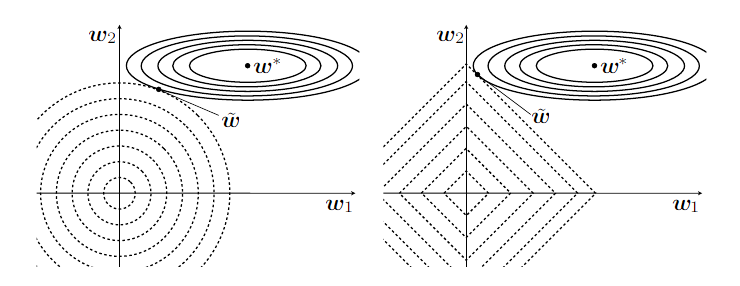
\includegraphics[width=0.8\linewidth]{images/4_regularizer}
\caption[]{Effekt der $L^2$- (links) und $L^1$-Norm (rechts) auf den Wert der optimalen Gewichte $W$ mit empirischem Optimum $W^*$ \cite[vgl.][Kap. 7.2, S. 199]{Bengio2015}}.
\label{fig:4_regularizer}
\end{figure}


\subsubsection{$L^1$-Norm}

Bei der Verwendung der $L^1$-Norm zur Berechnung von $\Omega(\Theta)$ bleibt nach dem Ableiten lediglich das Vorzeichen $sign(w_i)$ der einzelnen Gewichte übrig. Damit ergibt sich die in Gleichung \ref{eq:reg1} dargestellte Regel für die Berechnung des neuen Gradienten $\nabla_w \hat{J}(W,b)$ pro Gewicht $w$ \cite[vgl.][Kap. 7.2, S. 203 f.]{Bengio2015}. 

\begin{equation}
\label{eq:reg1}
\nabla_w \hat{J}(W,b) = \nabla_w J(W,b) + \alpha sign(w)
\end{equation}

Die $L^1$-Regu\-lari\-sierung bestraft die Summe aller Absolutwerte der Gewichte und verkleinert diese somit  während des Gradientenabstiegs stetig mit gleicher Rate. Die rechte Grafik in Abbildung \ref{fig:4_regularizer} zeigt, dass $L^1$-Regu\-lari\-sierung einerseits zu größeren Werten führt, im Gegenzug jedoch auch sehr kleine Werte bevorzugt. Diese Eigenschaft führt zu \textit{Sparsity}, da kleine Gewichte $w$ zwangsläufig im Laufe des Trainings den Wert Null annehmen \cite[vgl.][Kap. 7.2, S. 203]{Bengio2015}.
Die bayesianische Interpretation der Methode ist die A-priori Annahme einer isotropischen Laplace-Verteilung der Gewichte \cite[vgl.][Kap. 7.2, S. 206]{Bengio2015}.

\subsubsection{$L^2$-Norm}
\label{ch:l1_l2}
Trotz der interessanten \textit{Sparsity} Eigenschaften der $L^1$-Regularisierung wird im Deep Learning meist die $L^2$-Norm zur Regularisierung  verwendet und die \textit{Sparsity} mit ReLu-Funktionen erzwungen \cite[vgl. z.B.][]{Krizhevsky2012}.
Diese aus der \textit{Ridge Regression} bekannte Form der Regularisierung, führt zu Parameterwerten näher dem Ursprung. In der bayesianische Interpretation entspricht diese somit einer Gauß-Verteilung mit Mittelwert Null \cite[vgl.][Kap. 7.2, S. 200]{Bengio2015}. Der Gradient der $L^2$ regularisierten Fehlerfunktion ist in Gleichung \ref{eq:reg2} aufgeführt.

\begin{equation}
\label{eq:reg2}
\nabla_w \hat{J}(W,b) = \nabla_w J(W,b) + \alpha w
\end{equation}

Diese Form der Regularisierung führt dazu, dass das Modell eine größere Varianz in den Trainingsdaten $X$ annimmt. Somit werden Gewichte zu Merkmalen mit geringer Kovarianz zur Ausgabe verkleinert \cite[vgl.][Kap. 7.2, S. 200 f.]{Bengio2015}. Die \textit{Ridge Regression} in Gleichung \ref{eq:reg3} verdeutlicht diesen Aspekt, indem ein Vielfaches der Identitätsmatrix $I$ auf die Kovarianzmatrix $X^TX$ addiert wird.

\begin{equation}
\label{eq:reg3}
w = (X^TX + \alpha I)^{-1} X^Ty
\end{equation}


In Abbildung \ref{fig:4_regularizer} erkennt man diesen Effekt daran, dass das Gewicht $w_1$, in dessen Richtung die Zielfunktion im Gewichtsraum eher flach ist, geschrumpft wird.

\subsubsection{Max-$L^2$-Norm}

Max-$L^2$-Norm Regularisierung beschreibt eine Methode, welche die $L^2$-Norm der Gewichte eines Neurons $p$ beschränkt sodass $||w_p||_2 <= c$ gilt. Werte für den Hyperparameter $c$ liegen meist zwischen $3$ und $4$ \cite[vgl.][]{Srivastava2014}. Diese Art der Regularisierung projiziert folglich die Gewichte eines Neurons $w_p$ auf eine Kugel mit Radius $c$, sobald die Norm diese verlässt. 
Nach \cite{Srivastava2014} verhindert dies den \textit{Exploding Gradient}-Effekt, da die Gewichte den Fehler beim Rückpropagieren nicht mehr überproportional verstärken können. Dies ermöglicht größere Lernraten im Vergleich zum Training ohne Max-Norm-Re\-gu\-la\-ri\-sie\-rung, was gerade in Verbindung mit Dropout-Learning (siehe Kapitel \ref{ch:dropout}) von Vorteil ist, da so größere Gebiete im Gewichtsraum untersucht werden können.

\begin{figure}[H]
\centering
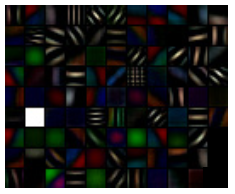
\includegraphics[width=0.4\linewidth]{images/4_max_norm}
\caption[]{Ein dominierender Filter ohne Max-Norm Regularisierung  \cite[siehe][]{Zeiler2014}}.
\label{fig:4_max_norm}
\end{figure}

 Abbildung \ref{fig:4_max_norm} zeigt einen weiteren Grund für die Notwendigkeit dieser Form der Regularisierung. Die Dominanz eines Filters über alle anderen kann effektiv verhindert werden \cite[vgl.][]{Zeiler2014}.




\subsection{Modellkapazität}
Beim Training großer Modelle mit hoher Kapazität ist \textit{Overfitting} von zentraler Bedeutung. \textit{Overfitting} beschreibt den Effekt eines kleiner werdenden Fehlers auf den Trainingsdaten bei gleichzeitiger Verschlechterung der Performanz auf den Testdaten. Abbildung \ref{fig:4_overfitting} stellt diesen Effekt grafisch dar.

\begin{figure}[H]
\centering
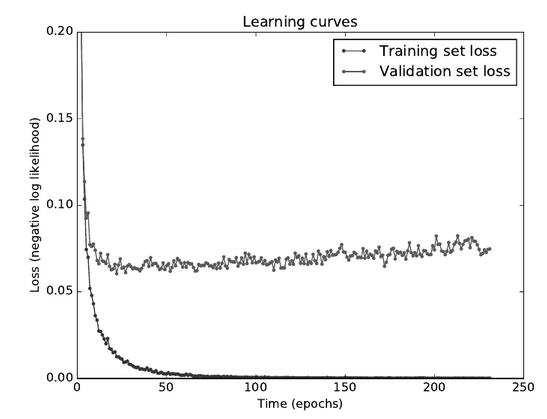
\includegraphics[width=0.4\linewidth]{images/4_overfitting}
\caption[]{\textit{Overfitting} am Beispiel des MNIST-Datensatzes \cite[siehe][Kap. 7.3, S. 216]{Bengio2015} }.
\label{fig:4_overfitting}
\end{figure}

Im Folgenden werden Methoden zusammengefasst, welche die Kapazität des Modells regulieren und damit aktiv versuchen \textit{Overfitting} zu verhindern.



\subsubsection{Early Stopping}
Die einfachste, sehr häufig angewandte Methode \textit{Overfitting} aktiv zu verhindern, ist das sogenannte \textit{Early Stopping}. Diese Methode teilt die Trainingsmenge zuerst in zwei Teilmengen. Sie setzt somit einen Satz Validierungsdaten voraus \cite[vgl. hierzu und im Folgenden][Kap. 7.3, S. 216 ff.]{Bengio2015}.

Beim \textit{Early Stopping} wird während des Trainings in regelmäßigen Abständen der Fehler auf den Validierungsdaten beobachtet. Verbessert sich dieser, werden die aktuellen Gewichte und Schwellwerte des Modells gesondert gespeichert. Am Ende des Trainings werden folglich nicht die aktuellsten Gewichte zurück\-gegeben sondern diejenigen, welche den kleinsten Validierungsfehler erzeugten.
Anstelle eines lokalen Minimums über den Trainingsdaten wird somit ein lokales Minimum des Validierungsfehlers gesucht. Das Training stoppt, sobald sich der Validierungsfehler über mehrere Epochen nicht verbessert hat (\textit{Early Stopping Patience}). Die Kapazität des Modells wird dahingehend beschränkt, dass die Trainingszeit limitiert ist.
Bei der $L^2$-Regularisierung wurde beobachtet, dass Gewichte in Richtungen hoher Krümmung hinsichtlich der Zielfunktion weniger stark reguliert werden als andere. Diese Beobachtung lässt laut \cite{Bengio2015} eine Ähnlichkeit zum \textit{Early Stopping} erkennen, da die Gewichte in Verbindung mit hoher Krümmung relativ zu den anderen Gewichten früher im Trainingsprozess gelernt werden.

\subsubsection{Parameteranzahl limitieren}
Die Kapazität des Modells lässt sich ebenso durch Vereinfachung beziehungsweise Verkleinerung und somit einer Verringerung der zu lernenden Gewichte regulieren. Im Umfeld des Deep Learning werden grundsätzlich zwei verschiedene Methoden beschrieben: Teilen der Gewichte (\textit{Parameter Sharing}) und Reduktion der Verbindungen zwischen Merkmalen. \\

\textit{Parameter Sharing} \\
Diese Methode ist am meisten verbreitet in CNNs und die Grundlage für die großen Erfolge im maschinellen Lernen und Deep Learning. CNNs berechnen an verschiedenen Stellen des Eingabebeispiels mit den selben Gewichten eine gewichtete Summe, was der algebraischen Faltung entspricht \cite[vgl.][]{LeCun1998}. 
Durch \textit{Parameter Sharing} ist es möglich große neuronale Netze zu trainieren, ohne die Trainingsmenge entsprechend zu vergrößern. Damit sind CNNs ein herausragendes Beispiel für die Integration von Expertenwissen in einem neuronalen Netz \cite[vgl.][Kap 7.8, S. 224]{Bengio2015}. \\

\begin{figure}
\centering
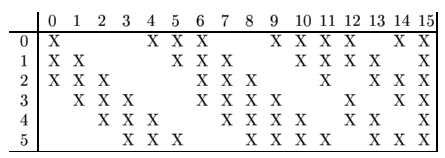
\includegraphics[width=0.4\linewidth]{images/4_connections}
\caption[]{Verbindungsmatrix der Merkmale beziehungsweise \textit{Feature-Maps} (Zeilen) mit den dazugehörigen Gewichten beziehungsweise Faltungsmasken (Spalten) zweier aufeinanderfolgenden Schichten \cite[siehe][]{LeCun1998}}.
\label{fig:4_connections}
\end{figure}

\begin{figure}
\centering
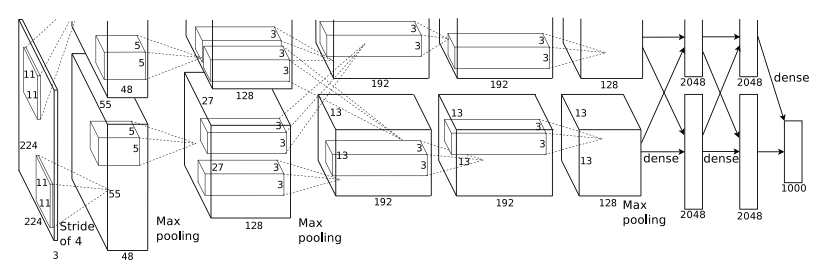
\includegraphics[width=0.9\linewidth]{images/4_Kriz}
\caption[]{Architektur für \textit{ImageNet 2012} mit limitierten Verbindungen zwischen \textit{Feature-Maps} zwecks Parallelisierung  \cite[siehe][]{Krizhevsky2012}}.
\label{fig:4_Kriz}
\end{figure}

\textit{Limitierung von Verbindungen zwischen Merkmalen} \\
Bei Nutzung diese Methode wird ebenfalls das Ziel verfolgt Parameter zu reduzieren, wobei allerdings ein anderer Ansatz als bereits vorgestellt gewählt wird. Anstatt die Eingabe nur in über\-lapp\-ende, rezeptive Felder zu unterteilen und mit den selben Gewichten zu gewichten, werden zusätzlich die unterschiedlichen Dimensionen der Eingabe (z. B. RGB-Kanäle) überlappend aufgeteilt. Die bekannte Verbindungsmatrix von \textit{LeNet 5} ist zur Veranschaulichung in Abbildung \ref{fig:4_connections} dargestellt.
Neben der Reduktion von zu trainierenden Gewichten erlaubt dies auch eine bessere Extraktion unabhängiger Merkmale \cite[vgl.][]{LeCun1998}. Darüber hinaus bedient sich die Architektur von \cite{Krizhevsky2012} zwecks Parallelisierung des Netzes auf mehrere Rechenkerne (hier GPUs) derselben Methode, wie Abbildung \ref{fig:4_Kriz} zeigt.\\


\subsubsection{Dropout}
\label{ch:dropout}
Die Dropout-Methode wurde von \cite{Hinton2012} eingeführt und bezeichnet eine Methode, mehrere kleinere Modelle zu lernen und die verschiedenen Ausgaben zu kombinieren (\textit{Model Averaging}). Hierbei ist hervorzuheben, dass dies gleichzeitig und in einem neuronalen Netz geschieht. \cite[vgl.][]{Srivastava2014}.

Die Dropout-Methode wurde mit dem Ziel entwickelt MLPs wenigen Trainingsdaten zu trainieren, was typischerweise in \textit{Overfitting} resultiert. Hierbei soll die Architektur des Netzes im Training zufällig für jedes Trainingsbeispiel verändert werden, um Abhängigkeiten (\textit{Co-Adaptions}) extrahierter Merkmale zu vermeiden \cite[vgl.][]{Hinton2012}. Dazu werden zufällig einzelne Neuronen deaktiviert. Dieses Grundprinzip ist in Abbildung \ref{fig:4_dropout} dargestellt. Um den Gradienten richtig zu berechnen, ist es wichtig, dass die deaktivierten Neuronen auch im Backpropagation beim \textit{Backward Pass} deaktiviert bleiben.

Wird das zufällige ausschalten von Neuronen deaktiviert, existiert ein trainiertes Netz, welches implizit mehrere Modelle kombiniert und somit eine deutliche Verbesserung gegenüber bestehenden Regularisierungsmethoden hinsichtlich \textit{Overfitting} darstellt \cite[vgl.][]{Srivastava2014}. Damit die Gewichte durch die Kombination der Modelle im Testlauf nicht zu groß sind, müssen diese mit ${1-p}$ skaliert werden. 
Als Hyperparameter muss für Dropout lediglich die Wahrscheinlichkeit $p$ ein Neuron zu deaktivieren angegeben werden. Typische Werte reichen von $0.1$ bis $0.5$ (vgl. \cite{Krizhevsky2012}, \cite{Srivastava2014} oder \cite{Simonyan2014}).

Wird die Standardinitialisierung in Verbindung mit ReLu-Funk\-tionen verwendet, muss darauf geachtet werden, dass die Neuronen positive Ausgaben erzeugen, um ebenso positive Gradienten für das Lernen zu erhalten. Dies kann mittels des Schwellwertes $b=1$ oder einer hinreichend großen Varianz erreicht werden \cite[vgl.][]{Hinton2012}.

Die beschriebene Methode kann auch bestehende, gut funktionierende Netze verbessern. Da die effektive Kapazität durch Dropout verringert wird, ist es sinnvoll die Anzahl existierender Neuronen $n$ auf $n/(1-p)$ zu erhöhen \cite[vgl.][]{Srivastava2014}. Aufgrund der Tatsache, dass CNNs die Modellkapazität durch \textit{Parameter Sharing} bereits stark regulieren, ist Dropout in Convolution-Layer nicht gleichermaßen effektiv wie in Hidden-Layer \cite[vgl.][]{Hinton2012}.	

\begin{figure}
\centering
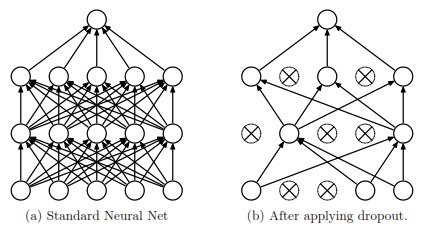
\includegraphics[width=0.6\linewidth]{images/4_dropout}
\caption[]{Schematische Darstellung eines gewöhnlichen MLP (links) und eines Dropout-MLP (rechts) \cite[siehe][]{Srivastava2014}}.
\label{fig:4_dropout}
\end{figure}			
	
\subsubsection{Padding im Convolution-Layer}
Wird in den Convolution-Layern die Eingabe bzw. die Ausgabe an den Rändern mit $(K - 1) / 2$ Nullen erweitert (Padding), verändert der Convolution-Layer nicht die Größe der Eingaben. Gerade bei der Verwendung von großen Filtermasken, wie beispielsweise $K = 7$, verhindert diese Methode eine schnelle Verkleinerung der Größe der Ausgabe. Damit wird auch verhindert, dass die Informationen an den Rändern der Eingabe früh im Netz verblassen \cite[vgl.][]{Kaparthy2014}. \\
		
				
\subsection{Erweitern der Trainingsdaten}
Die Kapazität eines Modells ist im Allgemeinen eine relative Größe basierenden auf der zur Verfügung stehenden Trainingsmenge. Folglich lässt sich das Problem des \textit{Overfittings} auch umgekehrt formulieren: Anstatt die Kapazität zu regulieren, kann die Menge der Trainingsdaten erhöht werden. Diese Methode wird häufig als \textit{Data Augmentation} bezeichnet und umfasst drei Bereiche: Affine Transformationen, Elastische Transformationen und Additives Rauschen. Diese Formen der Regularisierung haben oftmals großen Einfluss auf die Performanz des Systems hinsichtlich Invarianzen und müssen deshalb beim Vergleich unterschiedlicher Algorithmen und Lernmaschinen berücksichtigt werden.
\cite[vgl.][Kap. 7.5, S. 210 f.]{Bengio2015}



\subsubsection{Affine Transformationen}
Affine Transformationen können die Generalisierung des Netzes immens verbessern. Eingaben sollen hierbei so verändert werden, dass gewünschte Invarianzen besser trainiert werden. Dies ist auch dann von Vorteil, wenn das Modell selbst bereits gewisse Invarianzen, wie beispielsweise die Translationsinvarianz von CNNs, enthält. So finden affine Transformationen Anwendung im Training von \textit{LeNet 5} von \cite{LeCun1998} und im \textit{AlexNet} von \cite{Krizhevsky2012}.
Eine analytische Methode \textit{Data Augmentation} in den Trainingsprozess einzubauen, beschreibt \cite{Simard92} mittels des Tangent-Prop-Algorithmus.


\subsubsection{Elastische Transformationen}
Elastische Transformationen erweitern das Set an verfügbaren affinen Operationen und verbessern die Generalisierung dadurch weiter. 
Zunächst wird ein Vektorfeld pro Dimension generiert, welches zufällige Verschiebungen der einzelnen Eingabemerkmale (z. B. Pixel) beschreibt. Die generierten Felder werden anschließend mit einem Gauß-Kern gefaltet, beziehungsweise weichgezeichnet, und auf die originale Eingabe angewandt \cite[vgl.][]{Simard2003}.
Das Ergebnis elastischer Transformationen ist in Abbildung \ref{fig:4_elastic} dargestellt.

\begin{figure}
\centering
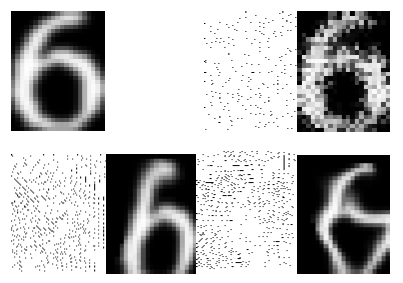
\includegraphics[width=0.5\linewidth]{images/4_elastic}
\caption[]{Originale Eingabe (oben links) und drei Beispiele elastisch veränderter Eingaben mit zugehörigem Vektorfeld \cite[siehe][]{Simard2003}}.
\label{fig:4_elastic}
\end{figure}


\subsubsection{Additives Rauschen}
Eine weitere Möglichkeit das System robuster zu machen, ist das Training mit additivem Rauschen. So korrumpiert beispielsweise \cite{Vincent2008} die Trainingsdaten zu einem gewissen Grad mit additiven Rauschen, Maskierung oder \textit{Salt-and-Pepper} und konstruiert damit einen \textit{Denoising Autoencoder} (DAE). Mehrere DAEs bilden zusammen \textit{Stacked Denoising Autoencoder} und schließen damit die Lücke zu den beschränkten Boltzmann-Maschinen und (DBNs) im Bereich des unüberwachten Vortrainings \cite[vgl.][]{Vincent2010}.

Gerade die Maskierung einzelner Merkmale im Eingaberaum liefert die Grundlage für das spätere Dropout, welches sowohl für die Hidden-Layer als auch im Input-Layer geeignet ist und die Generalisierung deutlich verbessern kann \cite[vgl.][]{Srivastava2014}.


\section{Visualisierungsmethoden}
Gerade die Verbindung von Bilderkennung und CNNs macht die Anwendung von Visualisierungsmethoden besonders attraktiv, da sich gewisse Verhaltensweisen des neuronalen Netzes so besser verstehen lassen.
Die meisten der vorgestellten Methoden haben das Ziel der Kritik, \textit{Features} aus neuronalen Netzen ließen sich nicht interpretieren, entgegenzuwirken \cite[vgl.][]{Zeiler2014}.

\subsection{Primitiv}

Die einfachste Möglichkeit des Sichtbarmachens des Neuronalen Netzes, ist die Visualisierung der Ausgabe beziehungsweise der Gewichte und wird deshalb als primitiv bezeichnet. Dennoch können diese Techniken wichtige Einblicke gewähren.

\subsubsection{Neuronen-Aktivierung}

Die Visualisierung der Ausgabe eines \textit{AlexNet} von \cite{Krizhevsky2012} ist in Abbildung \ref{fig:4_output} (links) dargestellt. Die Eingabe ist ein Bild einer Katze. Es fällt sofort auf, dass die Aktivierungen sehr dünnbesetzt (\textit{sparse}) sind, was letztendlich auf die ReLu-Funktionen zurückzuführen ist \cite[vgl.][]{Glorot2011}.

\begin{figure}
\centering
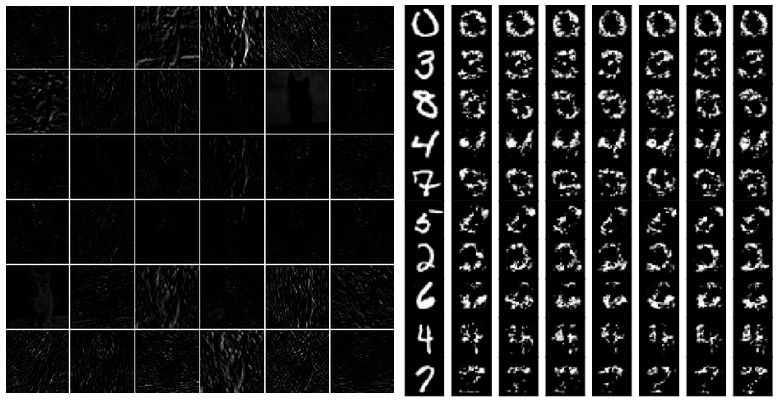
\includegraphics[width=0.6\linewidth]{images/4_output}
\caption[]{Aktivierungen des \textit{AlexNet} nach erstem Layer (links)  \cite[siehe][]{Kaparthy2014} und Rekonstruktionen eines Autoencoders (rechts) \cite[siehe][]{Vincent2010}}.
\label{fig:4_output}
\end{figure}

Diese Visualisierungsmethode kann in mehrerer Hinsicht unterstützen. Einerseits können so tote Neuronen identifiziert werden (vgl. \textit{Dying ReLu}-Effekt in \cite{Maas2013}). Andererseits kann überprüft werden, ob die Aktivierungen die gewünschte \textit{Sparsity} und Lokalität aufweisen.
Wird ein Autoencoder verwendet, kann darüber hinaus interessant sein, die Aktivierung beziehungsweise Ausgabe des Netzes zu visualisieren, da diese der Rekonstruktion der Eingabe entsprechen. Abbildung \ref{fig:4_output} (rechts) zeigt derartige Rekonstruktionen auf dem MNIST-Datensatz.

\subsubsection{Faltungskerne}
%http://eric-yuan.me/cnn/

Eine weitere einfache Möglichkeit, Informationen über das CNN zu erhalten ist die Visualisierung der gelernten Filtermasken. Abbildung \ref{fig:4_kernel} zeigt die Faltungskerne des ersten Layers eines trainierten \textit{AlexNet}. 

\begin{figure}[H]
\centering
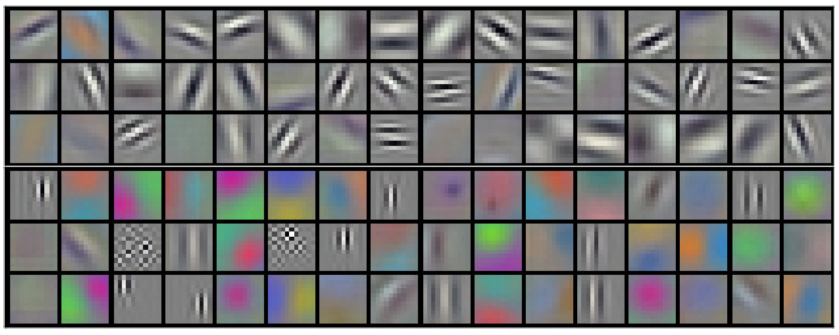
\includegraphics[width=0.5\linewidth]{images/4_kernel}
\caption[]{Die Faltungskerne des ersten Layers eines trainierten \textit{AlexNet}  \cite[siehe][]{Krizhevsky2012}}.
\label{fig:4_kernel}
\end{figure}

Trainierte Netze haben typischerweise glatte, Gabor-Filtern ähnliche Filtermasken. Verrauschte Filtermasken können hingegen entweder ein Indikator für eine fehlende Regularisierung und damit einhergehendes \textit{Overfitting} sein oder darauf hinweisen, dass das Netz nicht ausreichend konvergiert ist \cite[vgl.][]{Kaparthy2014}.     


\subsection{Gradientenbasiert}

Eine weitere Klasse von Visualisierungsmethoden arbeiten auf Basis des Backpropagation-Algorithmus. Dies bedeutet, dass sie sich der Fehler\-rück\-führung (\textit{Backward Pass}) bedienen und diese zur Visualisierung verwenden.

\subsubsection{Neuronen-Visualisierung}
Die erste Methode ist die sogenannte Deconvnet-Visualisierung von \cite{Zeiler2014}. Diese kann als Neuronen-Visualisierung bezeichnet werden, da letztlich Aktivierungen einzelner Neuronen visualisiert werden. Die Grundidee des Verfahrens ist es, einzelne Aktivierungen im Netz im Eingaberaum sichtbar zu machen. Dazu wird ein bestimmtes Neuron beziehungsweise eine bestimmte \textit{Feature-Map} ausgewählt und die Aktivierungen werden über die gesamte Testmenge gemessen. Die Beispiele mit den höchsten Aktivierungen werden gespeichert. Im Anschluss nutzt die Visualisierung diese Beispiele und rekonstruiert die erzeugten Aktivierungen, indem alle anderen \textit{Feature-Maps} dieses Layers Null gesetzt werden. Für die Rekonstruktion $R$ der Aktivierung wird im Grunde die Fehlerrückführung des Backpropagation-Algorithmus verwendet. Damit gilt in einem Convolution-Layer die Gleichung \ref{eq:zeiler1} zur Rekonstruktion einer Feature-Map.

\begin{equation}
\label{eq:zeiler1}
R^l_j = \sum_{i = 0}^{n} \hat{R}^{l+1}_{i} \ast rot180(W_{ij})
\end{equation}

Im Unterschied zur Berechnung des Gradienten mit Backpropagation, wird bei diesem Verfahren die Aktivierungsfunktion nicht abgeleitet. Stattdessen wird die Aktivierungsfunktion $\phi$ selbst mit der Rekonstruktion $R^{l+1}$ im Sinne des \textit{Forward Pass} berechnet. Formel \ref{eq:zeiler2} verdeutlicht diesen Zusammenhang für den Layer $l$.

\begin{equation}
\label{eq:zeiler2}
\hat{R}^{l+1}_i = \phi_l(R^{l+1}_i)
\end{equation}

Eine weitere Besonderheit stellen die Pooling-Layer dar, da diese im Prinzip nicht umkehrbar sind. Die von \cite{Zeiler2014} vorgeschlagene Methode sieht deshalb lediglich die Variante Max-Pooling vor und verbietet alle anderen Pooling-Verfahren. Max-Pooling bietet hierbei den Vorteil, dass im \textit{Forward Pass} die Stellen der Maxima vermerkt werden.

\begin{figure}
\centering
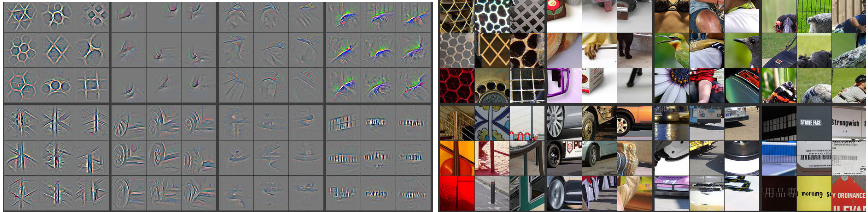
\includegraphics[width=0.9\linewidth]{images/4_zeiler}
\caption[]{Mit Deconvnet rekonstruierte Aktivierungen im dritten Layer (links) und dazugehörige originale Eingabebilder (rechts) \cite[siehe][]{Zeiler2014}}.
\label{fig:4_zeiler}
\end{figure}

Acht ausgewählte Neuronen im dritten Layer mit den jeweiligen zur höchsten Aktivierung korrespondierenden Eingabebildern, sind in Abbildung \ref{fig:4_zeiler} dargestellt.

\subsubsection{Saliency-Visualisierung}
%Gerneralized
Die sogenannte Saliency-Visualisierung von \cite{Simonyan2013} ist dem Deconvnet-Verfahren im Grunde sehr ähnlich. Es unterscheidet sich allerdings in einem zentralen Punkt. 
Während das Verfahren von \cite{Zeiler2014} Veränderungen im Vergleich zum Backpropagation-Algorithmus vornimmt, hält sich dieses Verfahren strikt an die Fehlerrückführung und berechnet damit die Ableitungen der Aktivierungsfunktionen, wie Formel \ref{eq:simonyian} zeigt. 

\begin{equation}
\label{eq:simonyian}
\hat{R}^{l+1}_i = R^{l+1}_i \circ \phi^{'}(z_i)
\end{equation}

Dies bietet den Vorteil, dass sich das Verfahren somit sowohl auf die Convo\-lution-Layer als auch die Hidden-Layer anwenden lässt. Dies lässt sich damit begründen, dass das Verfahren im ursprünglichen Sinne einzelne Klassen im Eingaberaum visualisiert \cite[vgl.][]{Simonyan2013}.


\begin{figure}
\centering
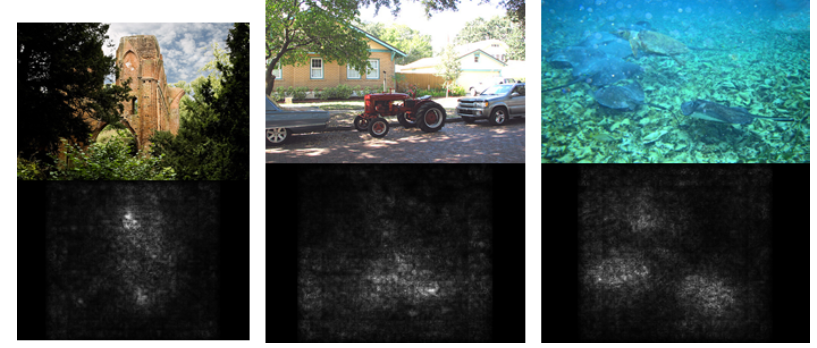
\includegraphics[width=0.6\linewidth]{images/4_simonyan}
\caption[]{Originale Eingabebilder (oben) und dazu gehörige \textit{Saliency-Maps} (unten) \cite[siehe][]{Simonyan2013}}.
\label{fig:4_simonyan}
\end{figure}

Abbildung \ref{fig:4_simonyan} zeigt die beschriebene Technik, angewandt auf Beispiele aus dem \textit{ImageNet}-Datensatz. Die \textit{Saliency-Map} zeigt die Rekonstruktion der entsprechenden Aktivierung im Output-Layer. 

\subsection{Nachverarbeitung}
Methoden im Bereich Nachverarbeitung sind dadurch charakterisiert, dass ein trainiertes MLP, beziehungsweise CNN, lediglich zur Erzeugung von Merkmalsvektoren oder zur Berechnung von Ausgaben herangezogen wird. Diese Art der Visualisierung beschränkt sich demnach auf den Kontext und betrachtet das Netz als \textit{Blackbox}, beziehungsweise als eine Funktion $h(x)$.


\subsubsection{t-SNE}

Die Methode t-Distributed Neighbor Embedding (t-SNE) beschreibt ein von \cite{Laurens2008} entwickeltes Optimierungsverfahren zur Dimensionsreduktion. Es verbessert das klassische SNE-Verfahren insofern, dass die Gradienten für die Optimierung einfacher zu berechnen sind. Darüber hinaus wird anstelle einer Gauß- eine Student-t-Verteilung als Ähnlichkeitsmaß im niedrigdimensionalen 2D oder 3D Zielraum verwendet \cite[vgl.][]{Laurens2008}. Der Grundmechanismus von t-SNE ist die Minimierung des Unterschieds zweier Wahrscheinlichkeitsverteilungen (Kullback-Leibler-Divergenz): Der Wahrscheinlichkeitsverteilung von Paaren im hochdimensionalen $P$ Raum sowie der im niedrigdimensionalen Raum $Q$. Damit ergibt sich die zu minimierende Zielfunktion $C$ in Formel \ref{eq:tsne}.


\begin{equation}
\label{eq:tsne}
C = KL(P||Q) ) = \sum_{i}^{} \sum_{j}^{} p_{ij} log(\frac{p_{ij}}{q_{ij}})
\end{equation}


\begin{figure}
\centering
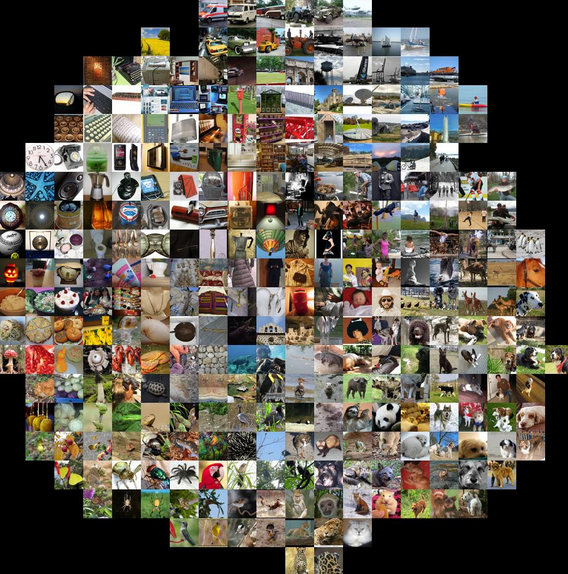
\includegraphics[width=0.5\linewidth]{images/4_t_sne}
\caption[]{t-SNE Einbettung einer Auswahl an \textit{ImageNet}-Bildern auf Basis der Aktivierung des letzten Layers im \textit{AlexNet} (Bild: Laurens van der Maaten, Facebook AI Research)}.
\label{fig:4_t_sne}
\end{figure}


Grundsätzlich können die von neuronalen Netzen erzeugten Merkmalsvektoren (\textit{Features}) auch mittels der Hauptkomponentenanalyse (PCA) visualisiert werden. Die t-SNE unterscheidet sich von PCA allerdings in einigen zentralen Eigenschaften \cite[vgl. hierzu und im Folgenden][]{Laurens2008}:

\begin{itemize}
\item Wenn ein Großteil der Varianz nicht in den ersten zwei, beziehungsweise drei, Hauptkomponenten beschrieben ist, kann t-SNE bessere Ergebnisse liefern, da es versucht die gesamte Information abzubilden.
\item t-SNE ist im Vergleich zur PCA keine orthogonale, lineare Transformation sondern eine nichtlineare Reduktion mit nicht zwingend orthogonalen Komponenten.
\item t-SNE findet, aufgrund der nicht-konvexen Zielfunktion, nicht immer zum globalen Minimum.
\item t-SNE ist darauf spezialisiert hochdimensionale Daten auf maximal zwei beziehungsweise drei Dimensionen zu reduzieren.
\end{itemize}



Abbildung \ref{fig:4_t_sne} zeigt die t-SNE 2D-Transformation des Merkmalsvektors vor dem Output-Layer eines \textit{AlexNet}. Als Eingabedaten dient eine Teilmenge des \textit{ImageNet}-Datensatzes. Diese Art der Visualisierung zeigt, dass das CNN Merkmale extrahiert und darauf aufbauend relevante von irrelevanten Merkmalen trennen kann. Dies lässt sich sehr deutlich daran erkennen, dass inhaltlich ähnliche Bilder näher zusammen sind als andere und somit Kategorien oder Gruppen und nicht Hintergrund oder Färbung die Daten charakterisieren \cite[vgl.][]{Bell2015}.


\begin{figure}
\centering
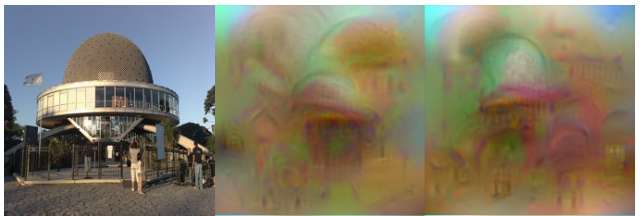
\includegraphics[width=0.5\linewidth]{images/4_inceptionismb}
\caption[]{Mögliche Rekonstruktionen des originalen Eingabebilds (oben links) \cite[siehe][]{Simard2003}}.
\label{fig:4_inceptionism}
\end{figure}

\subsubsection{Inceptionism}
Ein weiteres Verfahren, welches als \textit{Inceptionism}\footnote{Das Kunstwort \textit{Inceptionism} geht auf einen Blog-Eintrag von \textit{Research at Google} zurück (\url{http://googleresearch.blogspot.de/2015/06/inceptionism-going-deeper-into-neural.html} (26.08.2015)).} bezeichnet wird, wählt eine andere Herangehensweise. Durch Nutzung dieses Verfahrens wird versucht, ausgehend von einer Aktivierung, beziehungsweise einem Merkmalsvektor eines Layers, eine dazu passende Eingabe zu rekonstruieren. 
Das Grundverfahren, um Merkmalsvektoren zu invertieren, stammt von \cite{Mahendran2014}. Dieses Verfahren nimmt ein beliebiges Eingabebild $x_0$ und berechnet mittels eines trainierten CNN die Ausgabe $h_0 = h_l(x_0)$ in einem beliebigen Layer $l$. Das Ziel des Verfahrens ist es, die Zielfunktion $C$ in Gleichung \ref{eq:incept} mit Regularisierer $R(x)$ zu minimieren und ausgehend vom Rauschen ein optimales $x$ zu finden. 

\begin{equation}
\label{eq:incept}
C = ||h(x) - h_0||^2 + \lambda R(x)
\end{equation}

Der Regularisierer sorgt dafür, dass das optimale $x$ innerhalb eines für Bilder üblichen Intervalls $B = [-128,128]$ liegt (Formel \ref{eq:incept1}) und das resultierende Bild stückweise konstant ist (Formel \ref{eq:incept2}).

\begin{equation}
\label{eq:incept1}
R_1 = ||x||^6_6
\end{equation}

\begin{equation}
\label{eq:incept2}
R_2 = \sum_{i,j}^{} [(x_{i,j+1} - x_{ij})^2 + (x_{i+1,j} - x_{ij})^2)]^{\frac{1}{2}}
\end{equation}


Abbildung \ref{fig:4_inceptionism} zeigt fünf Optimierungen auf Basis des Eingabebilds oben links.



\chapter{Implementierung des Prototyps}
%- Implementierung										(13 Seiten)	(13 Seiten)
Nachdem in den vergangenen Kapiteln die theoretischen Grundlagen zu Convolutional Neural Networks (CNNs) gelegt wurden, widmet sich dieses Kapitel der Implementierung des Prototyps \textit{ConvNetCPP}. Es bildet somit die Basis für das darauffolgende Kapitel, in welchem die verschiedenen Aspekte des Prototyps hinsichtlich Deep Learning experimentell untersucht werden.
Der Prototyp setzt folgende Systemparameter voraus: \\

Systemvoraussetzungen und Abhängigkeiten:
\begin{itemize}
\item Python 3.4
\item SciPy \textemdash\space Scientific Python (siehe \cite{Scipy})
\item C++11
\item Eigen-Bibliothek für Lineare Algebra  (siehe \cite{eigenweb})
\item OpenMP kompatibler Compiler (siehe  \cite{openmp08})
\item Optional: Boost Bibliotheken (siehe \cite{Schling2011})
\end{itemize}

\textit{ConvNetCPP} unterstützt insgesamt folgende Funktionen:
\begin{multicols}{2}
\begin{itemize}
\item SGD  
\item Nesterov Momentum (NAG)
\item Rprop/RMSprop
\item Equilibrium SGD
\item AdaDelta
\item L1-/L2-/Max-Norm-Penalty
\item Dropout
\item MAX-/AVG-/Stochastic-Pooling
\item Ausgabe-\textit{Padding}
\item Early Stopping
\item Sig/Tanh/ReLu
\item Softmax-Regression
\item CE/MSE-Fehlermaß
\item Conv. Denoising Autoencoder
\item Neuronen-Visualisierung
\item Ausgabe-Visualisierung 
\item Kernel-Visualisierung
\end{itemize}
\end{multicols}

\section{Architektur}
%	- Architektur (Python c++ Extension)
%		- Klassen-Diagramm
%		- Computation Pipeline
%			- Grafik OpenMP
%			- Grafik Persistency Model Matrix
%			- Grafik Model Definition File
Die Architektur von \textit{ConvNetCPP} besteht aus zwei Teilen. Den in C++ implementierten Klassen sowie einem in C geschriebenen \textit{Python Module Extension}, welches die Schnittstelle zu Python darstellt.

\subsection{C++ ConvNet}
Der C++ Teil ist aufgeteilt in 9 Klassen, welche die unterschiedlichen Teile des CNN implementieren. Die Abhängigkeiten der Klassen sind in Abbildung \ref{fig:5_class_hierarchie_autoencoder} dargestellt.

\begin{figure}
\centering
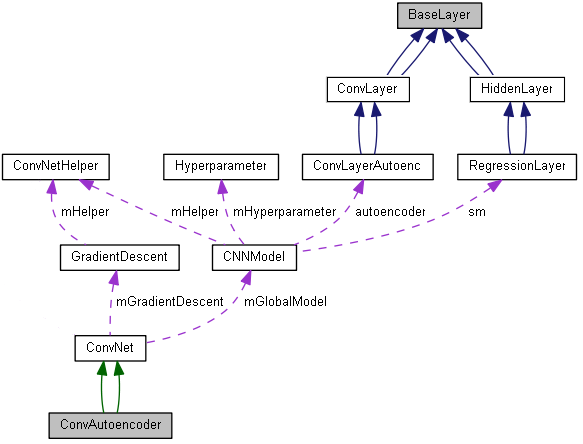
\includegraphics[width=0.8\linewidth]{images/5_class_hierarchie_autoencoder}
\caption[]{Klassenabhängigkeitsgraph des Prototyps (\textit{ConvNetCPP})}
\label{fig:5_class_hierarchie_autoencoder}
\end{figure}

Die Klasse ConvNetHelper beinhaltet die für ein CNN benötigten Basisfunktionalitäten wie das Drehen von Matrizen, Parallelisierung und die Konvertierung zwischen Vektoren und 3D-Daten für den Übergang zwischen Convolution- und Hidden-Layer. 

Optional kann die Abhängigkeit zu den Boost-Bibliotheken durch Angabe des Compiler-Flag \texttt{no\_serialization} aufgehoben werden. Damit wird die Serialisierung deaktiviert und der Status des Trainings nicht mehr länger persistiert. Dies bietet sich insbesondere unter Verwendung der Python API an, da hierbei der aktuelle Status des Models in Form einer 2D Datenstruktur an Python zurückgegeben werden.

Die vier zentralen Klassen \texttt{CNNModel}, \texttt{BaseLayer}, \texttt{ConvNet}, \texttt{ConvAutoencoder} und \texttt{Gradient\-Descent} werden im Folgenden genauer beschrieben. 

\subsubsection{CNNModel.cpp}
Die Klasse \texttt{CNNModel} repräsentiert das eigentliche CNN. Es beschreibt die Architektur und hält die Instanzen der entsprechenden Schichten des Netzwerks. 
Die Kommunikation zwischen den einzelnen Schichten geschieht mittels \textit{Messages} (vgl. Kapitel \ref{ch:cnn_back}). Diese \textit{Messages} werden durch die zwei Structs in Listing \ref{ls:struct} beschrieben. Eines definiert die Kommunikation bei der Berechnung der Netzaktivierung (\textit{Forward Pass}). Hierbei werden nur Pointer übergeben, da die entsprechenden Ausgaben pro Schicht für die Berechnungen des Gradienten weiter benötigt werden und dadurch keine Kopie der Eingabe pro Schicht erzeugt wird. Die \textit{Message} für die Rückpropagierung des Fehlers (\textit{Backward Pass}) wird nicht weiter benötigt, weshalb die Daten an die vorherige Schicht übergeben werden können.


\begin{lstlisting}[label=ls:struct,caption=Definitionen der Structs für die Kommunikation zwischen den einzelnen Schichten des CNN,captionpos=b]
struct ForwardMessage{
	vector<const vector<MatrixXd>*> vecData;
	MatrixXd* matData;
};

struct BackwardMessage{
	vector<vector<MatrixXd>> vecData;
	MatrixXd matData;
};
\end{lstlisting}

\subsubsection{BaseLayer.cpp}
Die abstrakte Klasse \texttt{BaseLayer} deklariert mehrere virtuelle Methoden, die von allen abgeleiteten Klassen implementiert werden müssen. Dies sind die für den Backpropagation-Algorithmus notwendigen Methoden für \textit{Forward Pass} und \textit{Backward Pass} sowie Methoden zur Visualisierung.
Darüber hinaus implementiert die Klasse die verschiedenen Aktivierungsfunktionen mit zugehörigen Ableitungen und Methoden zur Erzeugung gleich- oder normalverteilten Gewichten.


\subsubsection{ConvNet.cpp}
Die Klasse \texttt{ConvNet} bildet die Schnittstelle zum CNN nach außen und beinhaltet die gesamten Methoden zum Training, Prädiktion, Validierung und Visualisierung.
Die Methoden arbeiten auf Basis einer Instanz des \texttt{CNNModel}, welche außerhalb erzeugt werden muss und dem Konstruktor übergeben wird. 
Damit sind Steuerungslogik und Modelarchitektur voneinander getrennt.

\subsubsection{ConvAutoencoder.cpp}
Die Klasse \texttt{ConvAutoencoder} bildet die Schnittstelle zum Convolutional Autoencoder nach außen und beinhaltet die gesamten Methoden zum Vortraining, Prädiktion und Validierung. Die Klasse ist von \texttt{ConvNet} abgeleitet und arbeitet deshalb ebenso auf Basis einer Instanz des \texttt{CNNModel}, welche außerhalb erzeugt werden muss und dem Konstruktor übergeben wird. 

\subsubsection{GradientDescent.cpp}
Die Klasse \texttt{GradientDescent} implementiert den Gradientenabstieg und die verschiedenen Adaptionen wie Momentum und adaptive Lernraten. Da\-rüber hinaus ist in dieser Klasse auch die Max-Norm-Regularisierung implementiert, welche die Parameter unmittelbar nach einem Update auf die entsprechende Norm prüft und skaliert.
Sind die partiellen Ableitungen berechnet, wird die Instanz des \texttt{CNNModel} an \texttt{GradientDescent} übergeben und die entsprechenden Gewichtsupdates werden ausgeführt. Etwaige erweitere Algorithmen, wie das Schätzen der aktuellen Krümmung (siehe Equilibrium SGD), sind ebenfalls in dieser Klasse implementiert.


\subsection{Python Module Extension}
Python Module Extensions erlauben es in C/C++ implementierte Software in Python zur Verfügung zu stellen. Sie bilden die Standardvorgehensweise, um Python mit nativem Code zu erweitern.\footnote{Siehe dazu weitere Details in der offiziellen Python Dokumentation: \url{https://docs.python.org/3.4/extending/extending.html} (1.9.2015)}

Im Rahmen des Prototyps kann die CNN Funktionalität somit bequem durch das bereitgestellte Python Module verwendet werden, ohne auf die wichtige Performanz von nativem Code verzichten zu müssen.
Der folgende Teil beschreibt die grundlegende Konzeption der API und gibt einen Überblick der zur Verfügung stehenden Funktionen. Die Funktionen des CNN und des Convolutional Autoencoders sind aufgrund deren gemeinsamen Codebasis in einem Modul \textit{ConvNet} enthalten.

\subsubsection{Modellbeschreibung}
Im ersten Schritt wird das Modell spezifiziert. Für den Lebenszyklus eines Modells stehen die beiden Methoden \texttt{reset()} und \texttt{create()} zur Verfügung. Erstere Methode löscht bestehende Modelle, während letztere ein neues Modell erstellt.
Mehrere Modelle sind bereits vordefiniert. Spezielle Architekturen können mittels einer Konfigurationsdatei (vgl. Datei \texttt{/py\-/Model\-definition.py}) spezifiziert werden und als String der Methode \texttt{create()} übergeben werden. Dazu gehören Anzahl der Schichten, Neuronen und Zielklassen, Aktivierungsfunktionen, Dropout, Pooling, Padding sowie das Fehlermaß.

Eine weitere zur Beschreibung gehörende Methode ist \texttt{setHyperParameters()}. Diese erlaubt das Überschreiben der Standardparameter. Folgende  Hyperparameter werden bereitgestellt:

\begin{multicols}{2}
\begin{itemize}
\item INITIALIZATION
\item INIT\_STD\_DEVIATION
\item ALGORITHM
\item VISUALIZATION
\item THREAD\_COUNT
\item TRAINING\_COST\_PERIOD
\item FEATUREMAP\_DROPOUT
\item MATRIX\_CONVOLUTION
\item ENABLE\_INFO\_OUTPUT
\item ENABLE\_DEBUG\_OUTPUT 
\end{itemize}
\end{multicols}


Ist die Modellspezifikation abgeschlossen, kann ein zum Modell passender Parametersatz mit der Methode \texttt{loadState()} geladen werden.

\subsubsection{Training}
\label{ch:pytraining}
Bevor das Training gestartet werden kann, müssen die entsprechenden Trainingsparameter übergeben werden. Dies geschieht mittels der Methode \texttt{set\-Training\-Parameters()}. Folgende Parameter müssen angegeben werden:
\begin{multicols}{2}
\begin{itemize}
\item MAXITERATIONS  
\item BATCHES 
\item LRATE  
\item LRATE\_ALPHA
\item L2\_REG
\item L1\_REG
\item MAXNORM\_REG
\item MOMENTUM
\item LIMIT 
\item EARLY\_STOPPING
\item VALIDATION\_PERIOD
\item TRAIN\_VALID\_RATIO 
\end{itemize}
\end{multicols}

Das Training wird mit der Methode \texttt{fit()} gestartet. An dessen Ende werden die besten Parameter des Modells zurückgegeben und können gespeichert werden. Das Training kann so zu einem späteren Zeitpunkt fortgesetzt oder für Testzwecke verwendet werden.

\subsubsection{Unüberwachtes Vortraining}
Für unüberwachtes Vortraining sind speziell drei Hyperparameter wichtig, welche mittels der Methode \texttt{setAutoencoderParameters()} übergeben werden:

\begin{multicols}{2}
\begin{itemize}
\item TRAINING\_LAYER
\item INPUT\_DROPOUT\_RATE
\item FIX\_FIRST\_CONV\_LAYER
\end{itemize}
\end{multicols}

Das unüberwachte Vortraining wird durch den Aufruf der Methode \texttt{auto\-encoder\-\_fit()} gestartet, wobei die entsprechend zu trainierende Schicht angegeben werden muss. Im Anschluss werden die besten Parameter des Modells ebenfalls zurückgegeben und die gelernten Gewichte können dadurch als Initialisierung verwendet werden. Durch den Hyperparameter \texttt{FIX\-\_FIRST\-\_CONV\-\_LAYER} können die Gewichte der ersten Schicht des Netzwerks fixiert werden, um ein Überschreiben während des Trainings zu vermeiden.

\subsubsection{Validierung}
Zur Validierung des Modells werden die beiden Methoden \texttt{check()} und \texttt{autoencoder\_check()} angeboten. Diese liefern Informationen über die aktuellen Gradienten je Schicht, etwaige Hesse-Approximationen sowie über die Fehlerrate auf Test und Validierungsdaten.

\subsubsection{Prädiktion}
Die Methoden \texttt{predict()} und \texttt{autoencoder\_predict()} berechnen für beliebige neue Daten die entsprechende Prädiktion.

\subsubsection{Visualisierung} 
Zur Visualisierung des Modells stehen mehrere Methoden bereit. Zum einen primitive Methoden, die lediglich die Ausgabe und trainierte Parameter anzeigen: \texttt{getOutput()} und \texttt{getKernel()}. Darüber hinaus existieren auch komplexere gradientenbasierte Methoden. Diese umfassen einerseits die Visualisierung einzelner Neuronen (\texttt{visualize\-Neuron()}) oder der gesamten Ausgabe einer Schicht (\texttt{visualize\-Output()}). Die entsprechende Visualisierungsmethode wird als Hyperparameter definiert. Daneben kann die Methode \texttt{visualizeSample()} dazu verwendet werden, korrumpierte Ausgaben zu visualisieren.

\section{Implementierungsdetails}
Dieser Teil beschreibt wichtige Details in der Implementierung. Die beschriebenen Techniken vereinfachen die Berechnungen teilweise, beschleunigen diese oder können für das Debugging verwendet werden.

\subsection{Vereinfachungen}
Die Implementierung eines CNN lässt sich durch zwei Anpassungen deutlich vereinfachen.

\subsubsection{Korrelation statt Faltung}
Betrachtet man die Formeln des Backpropagation in Kapitel \ref{ch:cnn_back}, fallen einige Flip-Operationen ($rot180(\cdot)$) auf. Durch den Zusammenhang von Faltung und Kreuzkorrelation in Formel \ref{eq:correlation} kann so auf einige Flip-Operationen verzichtet werden. Das Symbol $\star$ bezeichnet die algebraische Kreuzkorrelation von Eingangssignal $x$ mit Filtermaske $y$.

\begin{equation}
\label{eq:correlation} 
x \star y = x \ast rot180(y)
\end{equation}

Werden alle Faltungen durch Kreuzkorrelationen ersetzt entfallen alle Flip-Operationen bei der Berechnung der partiellen Ableitungen. Die Flip-Oper\-ation für $\delta_{message}^l$ bleibt jedoch erhalten.

\subsubsection{Reverse Dropout}
Eine weitere nützliche Vereinfachung betrifft die Dropout-Methode. Das Standard-Dropout sieht vor im Testbetrieb die Gewichte mit $1-p$ zu skalieren \cite[vgl.][]{Srivastava2014}. 

Einfacher ist es allerdings die Testfunktion unverändert zu lassen und die Dropout-Methode gänzlich innerhalb des Trainings zu implementieren. Anstatt die Gewichte im Testbetrieb, also während Mittlung der einzelnen Dropout-Netze, zu verkleinern, werden die Gewichte während des Trainings mit $\frac{1}{1-p}$ vergrößert.

Eine Besonderheit muss allerdings hinsichtlich der Hyperparameter beachtet werden. Durch die vergrößerten Gewichte enthält der Gradient einen gewissen zusätzlichen Faktor, der bei der Wahl der Lernrate berücksichtigt werden muss.\footnote{Vgl. dazu \textit{Reproduce Geoff Hinton's MNIST dropout results in PyLearn2}: \url{https://github.com/lisa-lab/pylearn2/issues/193} (1.9.2015)}

\subsection{Vektorisierung}
Die Vektorisierung von Code ist hinsichtlich Performanz besonders wichtig. So kann die Verwendung von Vektor-Instruktionen wie des \textit{Intel Streaming SIMD Extension 2} die Berechnungen im Vergleich zu Schleifen deutlich beschleunigen. 
Da \textit{ConvNetCPP} eine Bibliothek für Lineare Algebra verwendet, welche die grundlegenden Funktionen wie Matrix-Matrix-Multiplikation (GEMM) bereits performant implementiert, ist es naheliegend zu versuchen so viele Berechnungen wie möglich auf GEMM zu reduzieren.

\subsubsection{Hidden-Layer}
In Kapitel \ref{ch:mlp} wurde bereits vorgestellt wie eine Schicht eines MLP mit $\phi(Wx + b)$ berechnet werden kann. Anstelle die einzelnen Neuronen-Aktivierungen mittels For-Schleife zu berechnen, wird die gesamte Schicht mit einer GEMM-Operation berechnet. 

Da im Rahmen von Deep Learning meist \textit{Mini-Batch}-Training angewandt wird, lässt sich die Vektorisierung zusätzlich noch auf mehrere Beispiele erweitern.
Im Falle eines Hidden-Layers werden die einzelnen Schichten mit Formel \ref{eq:vecminibatch} berechnet, wobei die Matrix $X$ einen \textit{Mini-Batch} mit $i$ Beispielen als Spaltenvektoren und die Matrix $B$ den um $i$ erweiterten Vektor mit Schwellwerten $b$ repräsentiert:

\begin{equation}
\label{eq:vecminibatch} 
\phi(WX + B)
\end{equation}

Dies lässt sich analog auf den \textit{Backward Pass} sowie die Berechnung des Gradienten übertragen. Damit lassen sich alle Berechnungen im Hidden-Layer jeweils mit GEMM-Operationen durchführen.

\subsubsection{Convolution-Layer}
In einem CNN fällt die meiste Rechenzeit in den Convolution-Layern an, weswegen es sich besonders lohnt auch hier die Berechnungen nach Möglichkeit auf GEMM-Operationen zu reduzieren \cite[vgl. im Folgenden][]{Caffee2015}. 

Der integrale Bestandteil eines Convolution-Layer ist die Berechnung der Faltung bzw. Kreuzkorrelation. Durch einen einfachen Trick lässt sich diese Berechnung für ein Trainingsbeispiel in eine GEMM-Operation überführen. Diese berechnet gleichzeitig alle \textit{Feature-Maps} aus allen \textit{Input-Maps}, wie Abbildung \ref{fig:5_convolution} anschaulich darstellt.

\begin{figure}
\centering
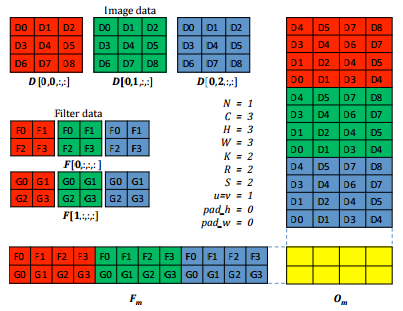
\includegraphics[width=0.6\linewidth]{images/5_convolution}
\caption[]{Schema der Faltung als Matrix-Matrix-Multiplikation (siehe \cite{Chetlur14})}
\label{fig:5_convolution}
\end{figure}

Die Reduktion funktioniert, indem einerseits die verschiedenen Filtermasken ausgerollt werden und andererseits Filtermasken, die zu einer \textit{Feature-Map} gehören hintereinander in einen Zeilenvektor konkateniert werden. Mehrere solcher Zeilenvektoren werden zu einer Matrix $F_m$ zusammengefasst. Außerdem müssen die einzelnen Bildausschnitte, welche mit den Masken gewichtet werden, ebenfalls ausgerollt und jede \textit{Input-Map} untereinander in einen Spaltenvektor konkateniert werden. Jede gültige Stelle der Eingabe wird so zu einer Matrix $I_m$ zusammengefasst. Als Ergebnis erhält man zwei Matrizen die mittels GEMM berechnet werden können. Die Berechnung eines Convolution-Layer wird so durch Formel \ref{eq:vecminibatch2} beschrieben, wobei entsprechend erweiterte Schwellwerte $B$ zur Anwendung kommen.

\begin{equation}
\label{eq:vecminibatch2} 
\phi(F_m I_m + B)
\end{equation}

Um wieder die Struktur der ursprünglichen Eingabe zu erhalten, müssen die resultierenden Zeilenvektoren $O_m$ nochmals entsprechend umorganisiert werden.
Diese Methode lässt sich auch auf \textit{Mini-Batch}-Training erweitert, indem mehrere Trainingsbeispiele analog zum Hidden-Layer spaltenweise konkateniert werden.

Grundsätzlich können Faltungsoperationen performant mittels der schnellen Fourier-Transformation im Frequenzbereich berechnet werden. Für die Anwendung im Bereich CNNs ist diese Methode allerdings nicht unbedingt von Vorteil, da beispielsweise die Filtergröße im Vergleich zur Eingabegröße gerade in den ersten Schichten sehr viel kleiner ist oder die Faltung mit größeren Schrittweiten (\textit{$Stride > 1$}) angewandt wird \cite[vgl.][]{Chetlur14}.

\subsection{Parallelisierung}
Betrachtet man die Verteilung der Rechenressource innerhalb eines CNN, fällt auf, dass 90 \% der Rechenzeit, aber nur 5 \% der Parameter auf die Convolution-Layer entfällt \cite[vgl.][]{Krizhevsky2014}. Daher bietet es sich an, die in \cite{Krizhevsky2014} vorgeschlagenen Strategien zu verwenden und zwar Daten-Parallelisierung in den Convolution-Layern und Modell-Paralleli\-sier\-ung in den Hidden-Layern.

Aus Gründen der Einfachheit und aufgrund der Tatsache, dass der CPU-basierte Prototyp für große Netze ohnehin nicht geeignet ist, wird auf Model-Parallelisierung verzichtet und das gesamte Netzwerk auf Basis der Daten parallelisiert. 
In \textit{ConvNetCPP} basiert die Parallelisierung auf OpenMP und damit auf parallel ausgeführten For-Schleifen. Ein \textit{Mini-Batch} wird somit auf die zur Verfügung stehende Threads aufgeteilt. Die Strategie ist unterteilt in drei Schritte.

\begin{enumerate}
\item Initialisierung \textemdash\space Jeder Thread bekommt eine Kopie der Modellarchitektur, inklusive eigenem Speicher für Gradient und Aktivierungen.

\item Parallelisierung \textemdash\space Der aktuelle \textit{Mini-Batch} wird auf die einzelnen Threads aufgeteilt und die Netzaktivierung (\textit{Forward Pass}) sowie die Gradientenberechnung (Backward Pass) werden lokal ausgeführt.

\item Zusammenführung \textemdash\space Die berechneten Gradienten werden über die Threads gemittelt und die Parameter aktualisiert.
\end{enumerate}


\subsection{Debugging}
\label{ch:debug}
Die Implementierung eines CNN oder eines Convolutional Autoencoder ist sehr fehleranfällig und im Allgemeinen schwierig zu debuggen. Eine sehr nützliche Methode die Richtigkeit der berechneten Gradienten in neuronalen Netzen zu überprüfen ist die Finite-Differenzen-Methode (vgl. z. B. \cite{Bouvrie2006}). Die Approximation zweiter Ordnung an die partiellen Ableitungen liefert eine bessere Genauigkeit und kann mit Formel \ref{eq:finitediff} berechnet werden (vgl. \cite{Bengio2012}).

\begin{equation}
\label{eq:finitediff} 
\frac{\partial J}{\partial w_i}  \approx \frac{J(w_i + \epsilon) - J(w_i - \epsilon)}{2 \epsilon}
\end{equation}

Mittels dieser Methode kann die Richtigkeit der im Convolutional Autoencoder (siehe Kapitel \ref{ch:autoenc}) gemachte Anpassung erfolgreich überprüft werden.

\chapter{Experimente}
\label{ch:experiment}
Trotz der vielen unterschiedlichen Techniken und Methoden aus dem letzten Kapitel, sind die Modelselektion und die Wahl der richtigen Methoden weiterhin sehr problemspezifisch.

Um für ein Lernproblem ein passendes Model zu finden, beschreiben \cite{Bengio2007b} drei essentielle Komponenten, die mit entsprechendem Vorwissen spezifiziert werden müssen:
\begin{enumerate}
\item Die Repräsentation und Vorverarbeitung der Daten

\item Die Architektur der Maschine oder des Neuronalen Netzes

\item Die Optimierung der Fehlerfunkion sowie Regularisierung
\end{enumerate}

Dieses Kapitel gliedert diese drei Komponenten in die Bereiche Modelselektion, Training und Visualisierung. Als Datenmaterial (vgl. Abbildung \ref{fig:6_samples}) dienen die beiden folgenden bekannten Datensätze:

\begin{itemize}
\item MNIST\footnote{MNIST-Datensatz: \url{http://yann.lecun.com/exdb/mnist/} (10.09.2015)} \textemdash\space Der MNIST-Datensatz handgeschriebener Ziffern besteht aus 60000 Trainingsbeispielen und 10000 Testbildern. Es stellt eine Untermenge des größeren NIST-Datensatzes dar. Die binarisierten Bilder sind $28 \times 28$ Pixel groß und die Ziffern zentriert. Richtwerte für Fehlerraten liegen mit \textit{Data Augmentation} bei 0.23 \% (\cite{Ciresan2012}), mit Vortraining bei 0.53 \% (\cite{Jarrett2009}) und ohne Vorverarbeitung bei 0.7 \% (\cite{Ranzato2006}). Das beste Ergebnis erreicht das \textit{DropConnect Network} von \cite{Zeiler2013} mit 0.21 \% Fehler ohne \textit{Data Augmentation}.

\item CIFAR-10\footnote{CIFAR-10-Datensatz: \url{http://www.cs.toronto.edu/~kriz/cifar.html} (10.09.2015)} \textemdash\space Der CIFAR-10-Datensatz besteht aus 50000 $32 \times 32 $ Pixel großen Trainingsbeispielen und 10000 Testbildern. Die Bilder sind aufgeteilt in 10 Klassen: Flugzeug, Auto, Vogel, Katze, Rotwild, Hund, Frosch, Pferd, Schiff und Lastwagen. Richtwerte für Fehlerraten liegen mit \textit{Data Augmentation} bei 9.3 \% (\cite{Zeiler2013}), ohne bei 11.7 \% (\cite{Goodfellow_maxout_2013}). Mit unüberwachten Vortraining erreichen \cite{Masci2011} 21.8 \%, ohne 22.5 \% Fehler.  Mit dem Standard Cuda-Convnet werden ohne \textit{Data Augmentation} und Vorverarbeitung ein Fehler von 18 \% erreicht\footnote{Cuda-Convnet Projekt: \url{https://code.google.com/p/cuda-convnet/} (10.09.2015)}. Das beste Ergebnis mit 8.2 \% Fehler erzielt das \textit{Deeply-Supervised Net} von \cite{Lee2014} mittels \textit{Data Augmentation}.
\end{itemize}

\begin{figure}
\centering
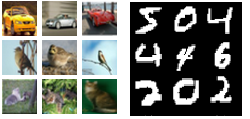
\includegraphics[width=0.5\linewidth]{images/6_samples}
\caption[]{CIFAR-10 Beispiele (links) und MNIST-Beispiele (rechts)}
\label{fig:6_samples}
\end{figure}


\section{Modelselektion}
Typischerweise bestehen die zur Verfügung stehenden Daten aus Trainingsdaten und Testdaten.
Um die verschiedenen Ergebnisse zu vergleichen, werden von den vorhandenen Trainingsdaten zufällige Beispiele entnommen. Wie Abbildung \ref{fig:6_validationset} zeigt, bilden diese Daten die Validierungsdaten, welche zur Überwachung des Trainings und zur Bestimmung der aktuellen Performanz verwendet werden. Die Testdaten werden verwendet, um das Model mit anderen Modellen zu vergleichen und dürfen nicht in die Validierung einbezogen werden \cite[vgl. z. B.][S. 222]{Hastie2009}. Eine Erweiterung zu diesem Verfahren ist die Kreuzvalidierung, wobei die Trainingsdaten in $k$ Blöcke unterteilt werden und das Training mehrfach mit unterschiedlichem Block zur Validierung durchgeführt wird. Die Performanz des Modells ergibt sich aus dem Durchschnitt der einzelnen Trainings \cite[vgl. z. B.][Kap. 7.2, S. 219]{Bengio2015}.  

\begin{figure}[H]
\centering

\includegraphics[width=0.6\linewidth]{images/6_validationset}
\caption[]{Aufteilung der Trainingsdaten in Trainings- und Validierungsdaten}
\label{fig:6_validationset}
\end{figure}

\subsection{Modelarchitektur}
Anfang der 2000er war es gängige Praxis die Anzahl der Parameter entsprechend der Menge an Trainingsdaten zu wählen
\cite[vgl.][S. 95 f.]{Zander2001}. 
Dies ist beispielsweise auch am bekannten \textit{LeNet 5} von \cite{LeCun1998} mit 60.000 freien Parametern für das Training des MNIST-Datensatzes zu erkennen.
Neuere vorgestellte Architekturen beinhalten deutlich mehr freie Parameter \cite[vgl. z. B.][]{Andrade2014}. Aufgrund besserer Techniken zur Regularisierung, wie beispielsweise Dropout, ist es möglich eine bedeutend größere Zahl an Gewichten als Trainingsdaten zu verwenden, ohne dabei mit \textit{Overfitting} konfrontiert zu werden \cite[vgl.][]{Bengio2012}.
Aufgrund empirischer Untersuchungen hat sich herausgestellt, dass die frühere angewandte Pyramidenform für die Layer-Größen (z. B. \textit{LeNet 5}: 6-16-120/84-10)\footnote{Die Darstellung der Modellarchitektur in der Form 6-16-120/84-10 steht für drei Convolution-Layer mit 6, 16, 120 \textit{Feature-Maps} und einem Hidden-Layer mit 84 sowie einem Output-Layer mit 10 Neuronen. Zur Klassifikation wird stets die Softmax-Regression angewandt.} suboptimal ist und gleichbleibende Größen der Schichten zu bevorzugen sind \cite[vgl.][]{Larochell2009}. 

Dieser Teil stellt die für die Experimente herangezogenen Architekturen der Modelle vor. In allen Experimenten werden, aufgrund ihrer guter Ergebnisse, die ReLu-Funktionen als Aktivierung und Max-Pooling als Pooling-Methode verwendet (vgl. z. B. \cite{Krizhevsky2012} und \cite{Simonyan2014}). Außerdem wird standardmäßig kein Padding angewandt. Dies bedeutet, dass die Größe nach einem Convolution-Layer mit Filtergröße $K \times K$ auf $N - K + 1 \times N - K + 1$ schrumpft.\\

\textit{LeNet 5+}\\
Die erste vorgestellte Architektur ist ein erweitertes \textit{LeNet 5} und orientiert sich an dem von \cite{Ranzato2006} vorgestellten Modell. 
Es wird mit 50-50/200-10 abgekürzt und umfasst im Detail die folgenden sechs Schichten:
\begin{enumerate}
\setlength{\itemsep}{0pt}
\item Convolution-Layer: 50 \textit{Feature-Maps} mit $5 \times 5$ Filtermasken
\item Pooling-Layer:	$2 \times 2$ Filtermasken
\item Convolution-Layer: 50 \textit{Feature-Maps} mit $5 \times 5$ Filtermasken
\item Pooling-Layer:	$2 \times 2$ Filtermasken
\item Hidden-Layer: 200 Neuronen
\item Output-Layer: 10 Neuronen mit Cross-Entropy Fehlermaß
\end{enumerate}
Dieses Netz wird für das Training der MNIST-Daten verwendet und umfasst für die Eingabe der Größe $28 \times 28 \times 1$ 63.750 Gewichte in den Convolution-Layern und 162.000 Gewichte im MLP. Insgesamt enthält es somit 223.950 Gewichte. \\

\textit{Net-7} \\
Das zweite vorgestellte Architektur besitzt eine zusätzliche Schicht und besteht folglich aus sieben Schichten. Es orientiert sich an den Modellen von \cite{Hinton2012} und \cite{Zeiler2013b}.
Das Modell wird mit 64-64-64/64-10 abgekürzt und umfasst im Detail die folgenden sieben Schichten:
\begin{enumerate}
\setlength{\itemsep}{0pt}
\item Convolution-Layer: 64 \textit{Feature-Maps} mit $5 \times 5$ Filtermasken
\item Pooling-Layer:	$2 \times 2$ Filtermasken
\item Convolution-Layer: 64 \textit{Feature-Maps} mit $5 \times 5$ Filtermasken
\item Pooling-Layer:	$2 \times 2$ Filtermasken
\item Convolution-Layer: 64 \textit{Feature-Maps} mit $5 \times 5$ Filtermasken
\item Hidden-Layer: 64 Neuronen
\item Output-Layer: 10 Neuronen mit Cross-Entropy Fehlermaß
\end{enumerate}
Dieses Netz wird für die CIFAR-10-Daten verwendet. Aufgrund der größeren Eingabe von $32 \times 32$ ist es möglich, drei Convolution-Layer zu verwenden, da nach zwei Convolution- und Pooling-Layern noch die Eingangsgröße von $5 \times 5$ für den dritten Convolution-Layer verbleibt. Dieses Netz umfasst für die Eingabe der Größe $32 \times 32 \times 3$ 209.600 Gewichte in den Convolution-Layern und 10.496 Gewichte im MLP.  Insgesamt enthält es somit 220.096 Gewichte. \\
%Parameters: 3*25*64 = 4800		32 - 4 = 28 / 2 = 14
%			64*64*25 = 102400	14 - 4 = 10 / 2 = 5 %
%			64*64*25 = 102400
%			64*64		= 4096
%			64*10			6400
%		=> 220 096

In diesem Zusammenhang ist die Analyse von \cite{Zeiler2014} von Bedeutung. Hier wird festgestellt, dass zum einen die Gesamttiefe des Netzes wichtig ist und zum anderen die Größe der Hidden-Layer keinen großen Einfluss auf die Performanz hat. Darüber hinaus hat die Größe der mittleren Convolution-Layer enormen Einfluss auf das Ergebnis, während ein zu großer Hidden-Layer nach den Convolution-Layern ohne Regularisierung zu \textit{Overfitting} führt.

%\subsubsection{Speicherbedarf}
%Da es allerdings nicht praktikabel ist, unnötige Rechenressourcen zu belegen, lohnt es sich dennoch das Modell möglichst klein zu halten. 	
%An dieser Stelle soll deshalb exemplarisch für den MNIST-Datensatz der für das \textit{LeNet 5+} benötigte Speicherplatz berechnet werden.
%Grundsätzlich ist der Speicherbedarf in zwei Kategorien einzuteilen: Aktivierungen und Gewichte und Schwellwerte.
%Für die Aktivierungen müssen nach den ersten Schicht $24*24*50=28.800$, nach der dritten Schicht $8*8*50=3.200$ und nach der fünften Schicht $200$ Aktivierungen gespeichert werden. Das macht inklusive der Eingabe bei doppelter Genauigkeit $257.944$ Bytes pro Trainingsbeispiel.
%Für die Gewichte und Schwellwerte sind entsprechend $(223.950 + 310)*8 = 1.794.080$ Bytes zu reservieren. Hinzukommt ein Faktor 4 für Gradient, Momentum und Hesse-Approximation. Insgesamt benötigt das Modell folglich 7.176.320 Bytes für die Parameter. Bei Parallelisierung multipliziert sich der benötigte Speicher entsprechend mit den Threads, wobei lediglich der Speicher für den Gradient extra berechnet werden muss.
%Die wichtigste Stellgröße für den Speicherbedarf ist somit die Wahl der Größe eines \textit{Mini-Batch}, da dieser unmittelbare Auswirkung auf den benötigten Speicher hat.


\subsection{Vorverarbeitung}
Die beiden verwendeten Datensätze werden auf verschiedene Arten vorverarbeitet. Somit werden mehrere Versionen erzeugt. Zunächst wird der Wertebereich beider Datensätze auf Werte zwischen 0 und 1 skaliert. Der MNIST-Datensatz wird im Anschluss lediglich zentriert, indem der Mittelwert pro Pixel subtrahiert wird. Der ebenfalls zentrierte CIFAR-10-Datensatz wird als CIFAR-10A bezeichnet. Eine zweite Variante, CIFAR-10B genannt, wird in den HSV-Farbraum\footnote{Der HSV-Farbraum bietet den Vorteil, dass die Farbe lediglich im H-Kanal codiert ist und die Kanäle S und V Informationen über Sättigung und Helligkeit enthalten.} transformiert und ebenfalls zentriert. 
\textit{Data-Augmentation} kann die Performanz immens verbessern. Hierauf wird allerdings im Folgenden verzichtet, da nicht die absolute Leistung des Modells von Interesse ist, sondern Unterschiede der einzelnen Aspekte und Methoden vorgestellt werden. 

Da im Rahmen der Experimente oftmals \textit{Early Stopping} zum Einsatz kommt, wird die Zentrierung der Daten lediglich mit den echten Trainingsdaten und nicht mit den Validierungsdaten berechnet. Im Anschluss werden die Validierungs- und Testdaten entsprechend transformiert. 


\section{Trainingsmethode}
Dieses Kapitel beschreibt die verschiedenen Experimente im Bereich des Trainings. Diese betreffen die Bereiche unüberwachtes Vortraining, Initialisierung, Gradientenabstieg und Regularisierung.

Als Größe für einen \textit{Mini-Batch} wird in Anlehnung an \cite{Bengio2012} immer eine Größe von 40 gewählt. Dies ermöglicht, dass bei 20 Threads jeweils zwei Trainingsbeispiele pro Thread parallel gerechnet werden können.
Zur Begrenzung der Trainingszeit sowie zur Vermeidung von \textit{Overfitting} kommt die Methode \textit{Early-Stopping} zum Einsatz. Wie zu Beginn des Kapitels beschrieben, müssen die Trainingsdaten dazu jeweils in ein Trainings- und Validierungsset unterteilt werden. Das Validierungsset umfasst stets 10 \% der Trainingsbeispiele und das Trainingsset somit entsprechend $55.000$ bei MNIST beziehungsweise $45.500$ bei CIFAR-10. \textit{Early-Stopping} wird derart verwendet, sodass das Modell immer fünf Durchläufe über das Trainingsset (Epochen) auf eine Verbesserung des Validierungsfehler wartet und das Training ansonsten abbricht. Im Anschluss gibt es verschiedene Varianten mit den verbliebenen Validierungsdaten umzugehen. \cite{Goodfellow_maxout_2013} beschreiben hierfür zwei Strategien: Bei Nutzung der ersten Strategie werden die Daten zur Trainingsmenge hinzugefügt und solange weiter trainiert bis der Validierungsfehler dem des Trainings entspricht. Wird die zweite Strategie verwendet, so wird das gesamte Training neu gestartet und solange trainiert bis der Trainingsfehler dem des Fehlers aus dem \textit{Early-Stopping}-Lauf entspricht. 

Im Rahmen dieser Arbeit wird allerdings die etwas praktikablere Methode von \cite{Ranzato2006} angewandt. Die Validierungsdaten werden hierbei ebenso am Ende des Trainings mit den Trainingsdaten kombiniert, jedoch wird maximal weitere 5 Epochen mit der gesamten Trainingsmenge trainiert. Das Training wird früher abgebrochen, falls sich der Validierungsfehler nicht weiter verbessert. Anschließend wird der Fehler auf den Testdaten berechnet, um die Ergebnisse der einzelnen Experimente zu vergleichen. 


\subsection{Vortraining}
\label{ch:pretrain} 
In diesem Teil soll das unüberwachte Vortraining untersucht werden. Dessen Ziel ist es, die erste Schicht im Modell zu initialisieren (vgl. z. B. \cite{Ranzato2006} und \cite{Masci2011}). Dabei sollen die enthaltenen Gewichte mittels des in Kapitel \ref{ch:autoenc} beschriebenen Convolutional Autoencoder trainiert werden. Alle Gewichte werden mittels der Standard-Initialisierung initialisiert (vgl. Kapitel \ref{ch:6_init}). Die Lernrate muss mit $\eta = 1^{-4}$ sehr klein gewählt werden, da das Modell im Rahmen dieser Experimente ansonsten divergiert. 

\subsubsection{MNIST}
Im ersten Experiment wird kein Input-Dropout, beziehungsweise keine Maskierung vorgenommen. Als Pooling-Methode kommt das Max-Pooling zum Einsatz. Die Trainingsdaten liefert der MNIST-Datensatz mit 55.000 Trainings- und 5.000 Validierungsbeispielen.
Bei Standard-Initialisierung und SGD mit einer Lernrate von $\eta = 1^{-4}$ erreicht das Model nach 39 Epochen ein Minimum mit einem MSE von $0.31$ auf den Testdaten.

Abbildung \ref{fig:6_mnist_autoencoder_combined} zeigt gelernte $5 \times 5$ Filtermasken der ersten Schicht auf der linken Seite.
\begin{figure}[H]
\centering
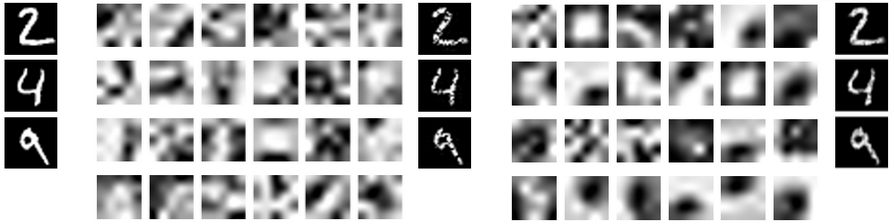
\includegraphics[width=0.9\linewidth]{images/6_mnist_autoencoder_combined}
\caption[]{Mit dem Convolutional Autoencoder trainierte Filtermasken und Rekonstruktionen der ersten \textit{LeNet 5+}-Schicht auf Basis des MNIST-Datensatz. Max-Pooling (links) und Max-Pooling und Maskierung (rechts)}
\label{fig:6_mnist_autoencoder_combined}
\end{figure}

Das zweite Experiment verwendet dieselbe Konfiguration, allerdings wird nun zusätzlich ein Input-Dropout von 30 \% verwendet.
Nach 14 Epochen erreicht das Modell einen MSE von $2.07$ auf den Testdaten. Abbildung \ref{fig:6_mnist_autoencoder_combined} zeigt die gelernten $5 \times 5$ Filtermasken der ersten Schicht auf der rechten Seite.
Die Filter des \textit{Denoising Autoencoder} aus dem zweiten Experiment wirken robuster und die Rekonstruktionen glatter. Deshalb werden diese für weitere Experimente beibehalten.

\subsubsection{CIFAR-10}
Im ersten Experiment wird kein Input-Dropout, beziehungsweise keine Maskierung vorgenommen. Als Pooling-Methode kommt ebenfalls das Max-Pooling zum Einsatz. Die Trainingsdaten stellt der CIFAR-10A/B-Datensatz mit 45.500 Trainings- und 4.500 Validierungsbeispielen.
Bei Standard-Initia\-lisierung und SGD mit einer Lernrate von $\eta = 1^{-4}$ erreicht das Modell auf den Testdaten (CIFAR-10A) nach 30 Epochen einen MSE von $74.06$ ohne Maskierung und $80.1$ mit Maskierung. Mit CIFAR-10B und Maskierung erreicht das Modell nach 20 Epochen einen deutlich besseren MSE von $26.2$ auf den Testdaten. 
Abbildung \ref{fig:6_cifar_autoencoder_combined_2} zeigt eine Auswahl der $5 \times 5$ Filtermasken der ersten Schicht in Graustufen. Es ist deutlich zu sehen, dass die Filter des CIFAR-10A optisch robuster wirken, während die Filter des CIFAR-10B sehr verrauscht sind.

\begin{figure}[H]
\centering
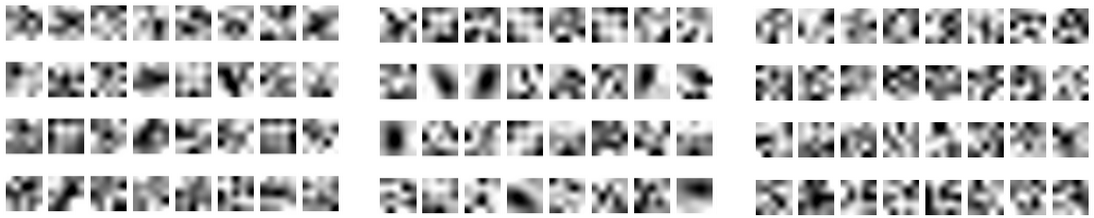
\includegraphics[width=1.0\linewidth]{images/6_cifar_autoencoder_combined_2}
\caption[]{Mit dem Convolutional Autoencoder trainierte Filtermasken der ersten \textit{Net-7}-Schicht auf Basis des CIFAR-10-Datensatz. CIFAR-10A: Max-Pooling (links), Max-Pooling und Maskierung (mitte) CIFAR-10B: Max-Pooling und Maskierung (rechts)}
\label{fig:6_cifar_autoencoder_combined_2}
\end{figure}

Für die weiteren Experimente werden jeweils die Filter aus dem Training mit Maskierung beibehalten.

\subsection{Initialisierung}
\label{ch:6_init}
In diesem Abschnitt werden verschiedene Initialisierungsmethoden verglichen. Als Basis dient in allen Beispielen der standardmäßige SGD mit einer \textit{Mini-Batch}-Größe von 40. Als Lernrate wird der universelle Wert $\eta = 0.01$ gewählt und es werden wieder 10 \% der Trainingsdaten zur Validierung verwendet. Tabelle \ref{tab:6_initialisierung} zeigt die jeweils erreichten Fehlerraten nach einer Epoche Training.

\begin{table}[H]

\centering
\begin{tabular}{c|c|c|c}
 	 			&   Standard		&  Xavier  	 	&  Vortraining 	 	\\ 
 	 			&     (mit $\sigma = 0.1$)		&  $~$  	 	&   (mit $\sigma = 0.1$)	 	\\ 
\hline MNIST 	&  	16.2/16.2 \%	&  	1.9/6.0   \% &  12.1/12.2 \%									\\
\hline CIFAR-10A&  	88.0/89.8 \%   &  	55.0/63.0 \% &  87.2/89.8 \%  				\\  
				&  	(68.4/72.2 \%)  &  	$~$ 		 &  (67.2/71.6 \%) 				\\  
\hline CIFAR-10B&  	88.0/89.8 \%	&  	54.6/62.2 \% &  87.2/89.8 \%		\\  
				&  	(66.8/71.4 \%)  &  	$~$ 		 &  (64.8/68.0 \%) 				\\  
\end{tabular} 
\caption{Fehler auf den Trainings-/Validierungsdaten nach einer Epoche (Ep.) Training}
\label{tab:6_initialisierung}
\end{table}

\subsubsection{Standard-Initialisierung}
Bei der Standard-Initialisierung werden alle Gewichte mit $W \sim \mathcal{N} (0,0.01)$ ini\-tialisiert. Abbildung \ref{fig:6_xavier_initialization} (mitte) zeigt pro Schicht die Verteilung der Werte im Gradienten über die erste Epoche beim Training des MNIST-Datensatz. Es fällt auf, dass die Varianzen über die verschiedenen Schichten gleich groß sind und somit kein \textit{Vanishing-Gradient}-Effekt erkennbar ist. Auch die angegebenen Fehlerraten in Tabelle \ref{tab:6_initialisierung} zeigen einen deutlichen Trainingsfortschritt.

\begin{figure}[H]
\centering
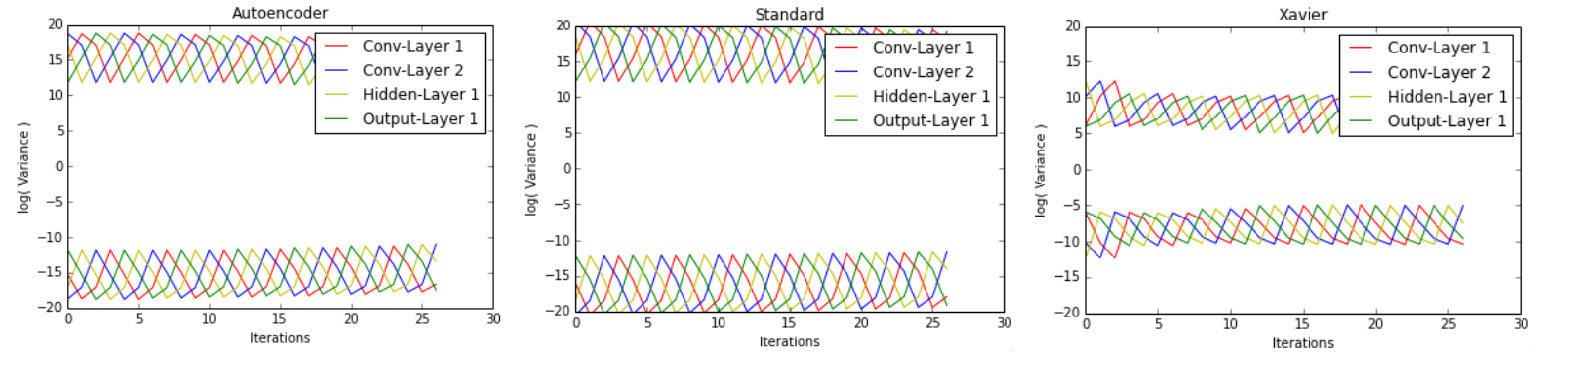
\includegraphics[width=1.0\linewidth]{images/6_xavier_initialization}
\caption[]{Log-Varianzen des Gradienten (gespiegelt) der einzelnen Schichten während der ersten Epoche des Trainings auf dem MNIST-Datensatz.}
\label{fig:6_xavier_initialization}
\end{figure}

Betrachtet man das Training mit CIFAR-10A/B in Abbildung \ref{fig:6_xavier_initialization_cifar}, zeigen die Varianzen der Werte im Gradienten ein ähnliches Bild wie beim MNIST. Allerdings sind die Varianzen hier kleiner (siehe Log-Varianz). Außerdem findet während der ersten Epoche kein erkennbarer Trainingsfortschritt statt. Dies deutet darauf hin, dass die Standard-Initialisierung nicht optimal für dieses Problem ist. Werden stattdessen die Gewichte mit $W \sim \mathcal{N} (0,0.1)$ initialisiert, sind die Varianzen größer und das Netz trainiert, was sich in den Werten in Tabelle \ref{tab:6_initialisierung} zeigt.


\subsubsection{Xavier-Initialisierung}
Bei der Xavier-Initialisierung werden alle Gewichte in Schichten mit ReLu-Aktivierungsfunktionen mittels $W \sim \mathcal{N} (0,\sqrt{2/fan_{out}})$ initialisiert. Die Abbildungen \ref{fig:6_xavier_initialization} und \ref{fig:6_xavier_initialization_cifar} (rechts) zeigt die Verteilung der Werte im Gradienten während der ersten Epoche pro Schicht. Im Vergleich zu den anderen Ini\-tialisierungstechniken sind die Varianzen insgesamt deutlich größer und das Modell erreicht bereits nach der ersten Epoche mit 6.0 \% (MNIST) respektive 63.0 und 64.2 \% (CIFAR-10A/B) sehr gute Fehlerraten auf den Validierungsdaten.

\subsubsection{Initialisierung durch Vortraining}
Nun werden die Gewichte mittels den gelernten Filtern aus Kapitel \ref{ch:pretrain} initialisiert. 
Die Abbildungen \ref{fig:6_xavier_initialization} und \ref{fig:6_xavier_initialization_cifar} (links) zeigen die Verteilung der Werte im Gradienten über die ersten Epoche pro Schicht. Beim MNIST-Datensatz ist zu erkennen, dass die Varianzen insgesamt zwar kleiner sind als bei der Xavier-Initialisierung, allerdings im Vergleich zur Standard-Initialisierung gegen Ende der Epoche größer werden. In der Folge führt diese Initialisierung zu einem besseren Ergebnis als bei Verwendung der Standard-Initialisierung, was Tabelle \ref{tab:6_initialisierung} zeigt. 
Anders verhält es sich beim CIFAR-Datensatz. Sowohl bei Verwendung der Datensätze CIFAR-10A/B als auch der Standard-Initialisierung findet in der ersten Epoche kein erkennbares Training statt und die Varianzen sind sehr klein. Analog zur Standard-Initialisierung findet ein Trainingsfortschritt statt, sobald die Standardabweichung im restlichen Netz auf $\sigma = 0.1$ erhöht wird. In diesem Modus erreicht das Netz binnen einer Epoche einen etwas geringeren Fehler als die gesamtheitliche Standard-Initialisierung.


\begin{figure}[H]
\centering
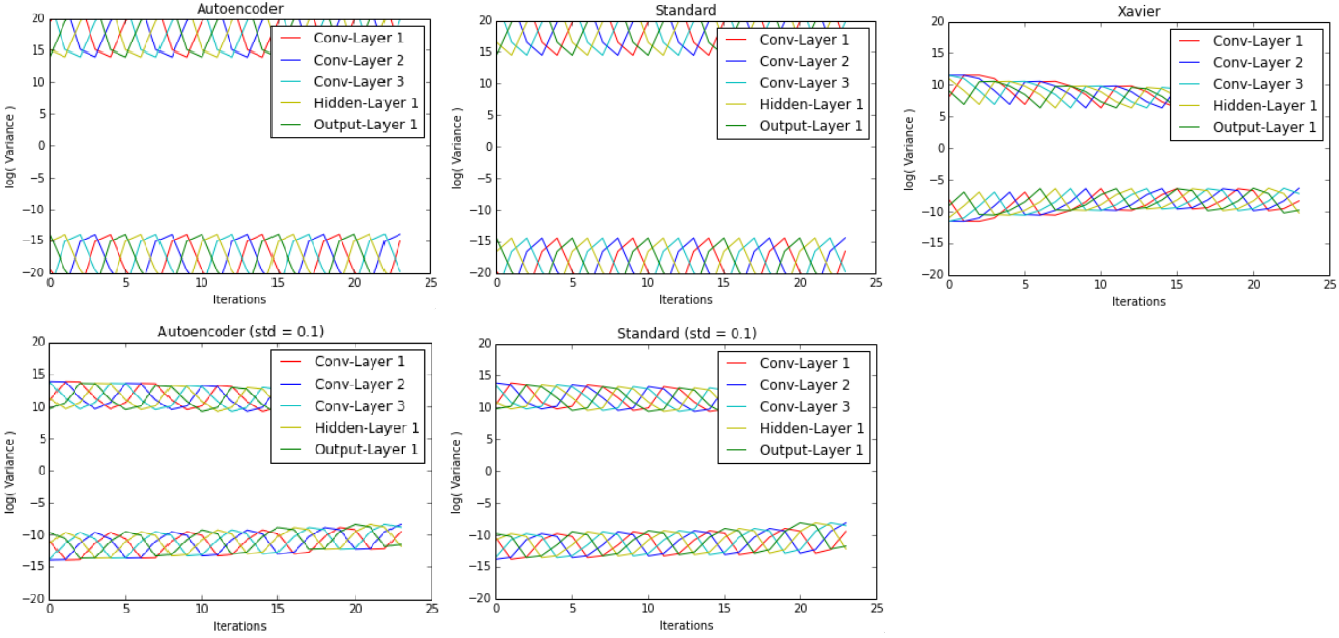
\includegraphics[width=1.0\linewidth]{images/6_xavier_initialization_cifar}
\caption[]{Log-Varianzen des Gradienten (gespiegelt) der einzelnen Schichten während der ersten Epoche des Trainings auf dem CIFAR-10A-Datensatz.}
\label{fig:6_xavier_initialization_cifar}
\end{figure}


\subsection{Gradientenabstieg}
In diesem Abschnitt werden die Adaptionen des Gradientenabstiegs untersucht, die im Rahmen dieser Arbeit von Relevanz sind. Zu diesen zählen SGD, Nesterov Momentum, RMSprop, AdaDelta und Equilibrium SGD. Da RMSprop den Equilibrium SGD sehr gut approximiert, bleibt letzterer im Folgenden unberücksichtigt. Im letzten Abschnitt konnte festgestellt werden, dass die Xavier-Initialisierung für beide Probleme eine geeignete Initialisierungsmethode darstellt. Die Experimente in diesem Teil werden deshalb mit dieser Methode initialisiert. Außerdem führt die Vorverarbeitung des CIFAR-10B-Datensatz zu einer konstanten, wenn auch kleinen, Verbesserung der Fehlerraten. Im folgenden wird deshalb lediglich der MNIST und CIFAR-10B-Datensatz betrachtet. Folgende Hyperparameter sind für alle Methoden gleich:

\begin{itemize}
\item 90 \% Trainings- und 10 \% Validierungsdaten
\item Lernrate $\eta = 0.01$
\item \textit{Early Stopping Patience} von fünf Epochen mit reduzierten Trainingsdaten und eine Epoche beim Training mit den kombinierten Trainingsdaten
\item Validierung des Modells nach jeweils 1000 Gradientenupdates (\textit{Mini-Batch}-Iterationen)
\end{itemize}

Im Rahmen der folgenden Experimente ist kein Absenken der Lernrate über das Training vorgesehen. Lediglich beim standardmäßigen SGD wird die Lernrate während des abschließenden Trainings mit kombinierten Daten auf $\eta = 0.001$ gesenkt, da diese Methode selbst keine Möglichkeit zur Veränderung der Lernrate besitzt. Neben dem \textit{Early-Stopping} werden keine weiteren Methoden zu Regularisierung verwendet. Die Tabelle \ref{tab:6_gradientdescent} zeigt eine Übersicht der jeweils erreichten Fehlerraten auf den Validierungs- und Testdaten.


\begin{table}
\centering
\begin{tabular}{c|c|c}
 	 			&   MNIST							& CIFAR-10B						 		\\ 
\hline SGD		&  0.40/0.82/0.93 \% (21 Ep.)	&	18.87/30.29/33.31 \% (27 Ep.)		\\
\hline Nesterov &  0.06/0.12/0.69 \% (11 Ep.)	&	17.77/28.94/34.01 \% (34 Ep.)				\\
\hline RMSprop  &  0.22/0.48/0.89 \% (10 Ep.)	&	29.03/37.74/41.92 \% (29 Ep.)				\\
\hline AdaDelta &  0.02/0.18/0.61 \% (12 Ep.)	&	20.86/21.99/36.65 \% (12 Ep.)				\\

%AdaDelta CIFAR 36.65
\end{tabular} 
\caption{Fehler auf den Trainings-/Validierungs-/Testdaten nach dem gesamten Training mit verschiedenen Methoden zum Gradientenabstieg}
\label{tab:6_gradientdescent}
\end{table}

In Abbildung \ref{fig:6_filters_mnist} sind Beispiele der Filter der ersten Schicht des \textit{LeNet 5+} nach dem Training mit dem MNIST-Datensatz dargestellt. Die Abbildung \ref{fig:6_filters_cifar} zeigt beispielhafte Filter der ersten Schicht des \textit{Net-7} nach dem Training mit den CIFAR-10B-Daten in Graustufen.

\begin{figure}
\centering
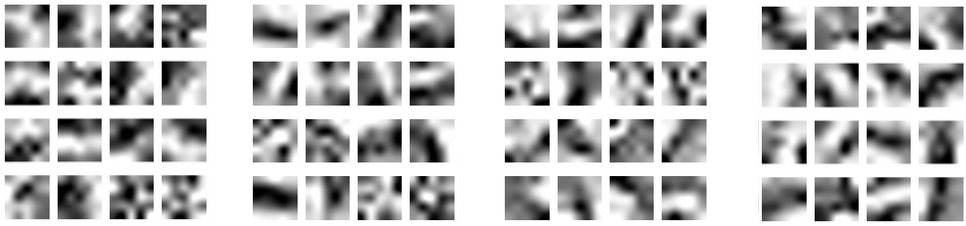
\includegraphics[width=0.7\linewidth]{images/6_filters_mnist}
\caption[]{Beispielhafte Filter der ersten Schicht des \textit{LeNet 5+}: SGD (links), Nesterov (mitte-links), RMSprop (mitte-rechts) und AdaDelta-Methode (rechts)}
\label{fig:6_filters_mnist}
\end{figure}


\begin{figure}
\centering
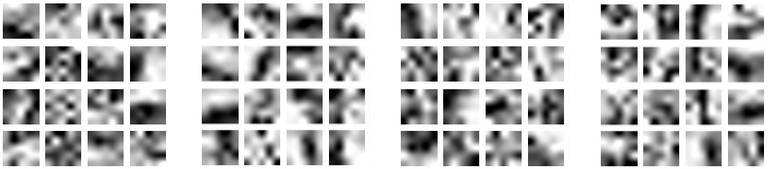
\includegraphics[width=0.7\linewidth]{images/6_filters_cifar}
\caption[]{Beispielhafte Filter der ersten Schicht des \textit{Net-7}: SGD (links), Nesterov (mitte-links), RMSprop (mitte-rechts) und AdaDelta-Methode (rechts)}
\label{fig:6_filters_cifar}
\end{figure}


\subsubsection{SGD}
Das Training auf den MNIST-Daten mit SGD dauert mit 21 Epochen im Vergleich zu den anderen Methoden sehr lange. Auch sind die erreichten Fehlerraten im Vergleich die schlechtesten. Die Abbildung \ref{fig:6_training_mnist} zeigt den Verlauf der Fehlerraten über das gesamte Training. 
Das Training mit den CIFAR-10B-Daten gestaltet sich schwieriger und dauert mit SGD 27 Epochen. Die SGD Methode erzielt im Rahmen dieser Experimente das zweitbeste Ergebnis. Allerdings ist dieses Ergebnis mit einer Fehlerrate von 33.31 \% relativ schlecht und das Training mit SGD insgesamt sehr langsam. Die Abbildung \ref{fig:6_training_cifar} zeigt den Verlauf der Fehlerraten über das gesamte Training.

\begin{figure}
\centering
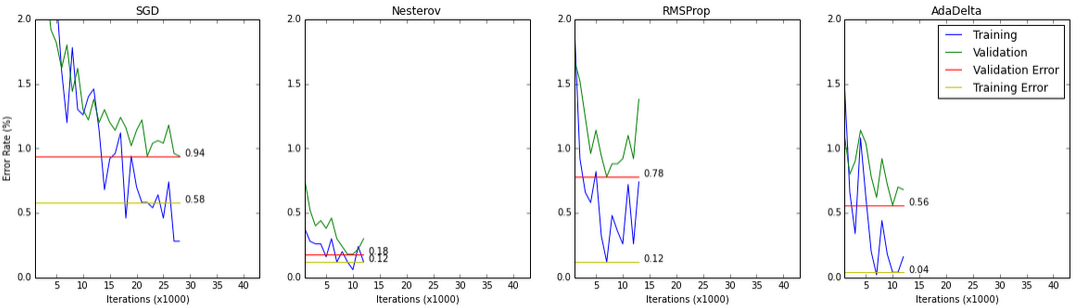
\includegraphics[width=1.0\linewidth]{images/6_training_mnist_2}
\caption[]{Trainings- und Validierungsfehler während des Trainings auf dem reduzierten MNIST-Datensatz mittels SGD-, Nesterov-, RMSprop und AdaDelta-Methode}
\label{fig:6_training_mnist}
\end{figure}


\subsubsection{Nesterov-Momentum}
Für das Training mittels Nesterov-Momentum wird als Hyperparameter für den Momentum-Term exemplarisch $\mu = 0.95$ gewählt \cite[vgl.][]{Sutskever2013}.
Das Training auf den MNIST-Daten ist deutlich beschleunigt und endet bereits nach 11 Epochen. Daneben weist es mit einem Testfehler von 0.69 \% die zweitbeste Fehlerrate auf.  
Beim Training mit den CIFAR-10B-Daten fällt auf, dass der Validierungsfehler kleiner ist als beim Training mit SGD, der Testfehler jedoch etwas höher. Das Training dauert mit 34 Epochen in Relation zu den anderen Methoden am längsten. Die Lernkurve ähnelt beim Training mit CIFAR-10B sehr jener des SGD, weist allerdings gegen Ende einen flacheren Verlauf auf und ist insgesamt weniger volatil.


\subsubsection{RMSprop}
Für das Training mit RMSprop werden folgende Werte exemplarisch als Hyperparameter gewählt \cite[vgl.][]{Dauphin2015}:
\begin{itemize}
\item $\rho = 0.90$
\item $\mu =10^{-2}$
\end{itemize}
Das Training mit RMSprop erreicht auf den MNIST-Daten nach 10 Epochen bessere Fehlerraten als der SGD, allerdings nicht so gute Ergebnisse wie die Methoden Nesterov-Momentum und AdaDelta.
Beim Training mit CIFAR-10B-Daten erzielt die RMSprop-Methode nach 29 Epochen die schlechtesten Ergebnisse im Rahmen dieser Experimente. Insgesamt weisen die Lernkurven im Vergleich zum Training mit Nesterov-Momentum einen volatileren Verlauf auf. Beim Training mit den MNIST-Daten fällt auf, dass die Fehlerraten nach dem Minimum sich sehr schnell verschlechtern.

\begin{figure}
\centering
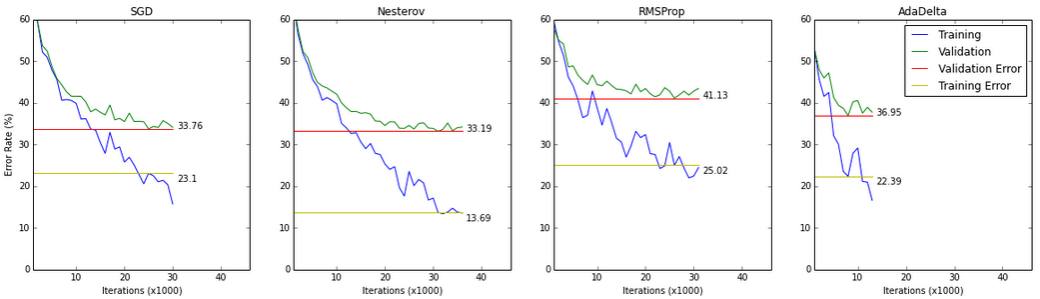
\includegraphics[width=1.0\linewidth]{images/6_training_cifar_2}
\caption[]{Trainings- und Validierungsfehler während des Trainings auf dem reduzierten CIFAR-10B-Datensatz mittels SGD-, Nesterov-, RMSprop und AdaDelta-Methode}
\label{fig:6_training_cifar}
\end{figure}

\subsubsection{AdaDelta}
Für das Training mit AdaDelta werden folgende Werte exemplarisch als Hyperparameter gewählt \cite[vgl.][]{Zeiler2012}:
\begin{itemize}
\item $\rho = 0.95$
\item $\mu = 10^{-6}$
\end{itemize}
Das Training mit AdaDelta erreicht auf den MNIST-Daten bereits nach 12 Epochen einen Testfehler von 0.61 \%. Damit erzielt die AdaDelta-Methode im Rahmen dieser Experimente die besten Ergebnisse. Ähnlich verhält es sich bei Durchführung des Experiments auf Basis der CIFAR-10B-Daten. Hier erreicht das Training mit der AdaDelta-Methode bereits nach 12 Epochen den besten Validierungsfehler und einen Testfehler im oberen Bereich. Auffällig ist, dass der Validierungsfehler beim Training mit den kombinierten Trainingsdaten sehr schnell fällt und sich damit das Modell rasch an die neuen Daten anpasst. Letztendlich handelt es sich hierbei jedoch um \textit{Overfitting}. Insgesamt weist das Training mit AdaDelta die höchste Volatilität in den Fehlerraten auf.


\subsection{Regularisierung}
Im letzten Abschnitt konnte festgestellt werden, dass der Validierungsfehler deutlich unter dem Testfehler liegt. Während das \textit{LeNet 5+} dennoch sehr gute Ergebnisse erzielt, zeigt das \textit{Net-7} bereits früh im Training eine Stagnation der Validierungsfehler. Dieses als \textit{Overfitting} bekannte Phänomen gilt es zu vermeiden. Begründen lässt sich dies damit, da ein solches Modell mit großer Sicherheit zu einem schlechteren Ergebnis auf unbekannten Daten führt, als ein regularisiertes Vergleichsmodell. In diesem Abschnitt gilt es daher entsprechende Techniken zur Regularisierung zu untersuchen.

Als Basis dient das \textit{Net-7} sowie der CIFAR-10B-Datensatz. Für den Gradientenabstieg wird die AdaDelta-Methode mit den Hyperparametern aus den vorhergegangenen Experimenten eingesetzt, da diese Methode gute Ergebnisse mit kurzer Trainingszeit erzielt. Als Referenzergebnis dienen 21.99/36.65 \% Fehlerrate auf den Validierungs-/Testdaten.
Auf die L1-Regularisierung wird im Folgenden verzichtet, da die erwünschte \textit{Sparsity} der Aktivierungen bereits durch die Verwendung von ReLu-Aktivierungsfunktionen erzielt wird (siehe. Kapitel \ref{ch:l1_l2}).
In Tabelle \ref{tab:6_regularisierung} sind die Ergebnisse der Experimente sortiert nach Testfehler aufgeführt.

\begin{table}
\centering
\begin{tabular}{c|c}
													&	 CIFAR-10B						\\ 
\hline MLP/1-Conv 0.3 \% + Max/L2 + Padd.		& 	27.61/27.06/28.41 \%	 	(21 Ep.)	\\
\hline MLP 0.3 \% + Max + Padd.				& 	16.68/21.51/29.69 \%	 	(36 Ep.)	\\
\hline MLP/1-Conv 0.3 \%  + Max + Padd.		& 	22.48/25.55/29.97 \%	 	(32 Ep.)	\\
\hline Dropout MLP 0.3 \%							& 	20.51/27.15/33.13 \% 		(20 Ep.)	\\
\hline Max-Norm-Regularisierung						& 	21.64/22.82/35.07 \% 		(18 Ep.)	\\
\hline L2-Regularisierung							& 	22.43/27.97/35.21 \% 		(21 Ep.)	\\
\hline Dropout MLP/1-Conv 0.3 \% + Max				& 	27.63/33.87/35.24 \% 		(44 Ep.)	\\
\hline Dropout MLP 0.5 \% + Max						& 	25.40/29.96/35.89 \% 		(20 Ep.)	\\
\hline Net-7 ohne Regularisierung					& 	20.86/21.99/36.65 \%		(12 Ep.)	\\
\hline Dropout MLP/1-Conv 0.5 \% + Max				& 	50.97/51.02/51.81 \% 		(27 Ep.)	\\
\end{tabular} 
\caption{Fehler auf den Trainings-/Validierungs-/Testdaten nach dem gesamten Training mit verschiedenen Methoden zur Regularisierung sortiert nach Testfehler}
\label{tab:6_regularisierung}
\end{table}


\subsubsection{L2-Regularisierung}
In diesem Experiment wird dem Modell die L2-Regularisierung hinzugefügt. Die Regularisierung wird dabei exemplarisch mit Parameter $\alpha = 0.0005$ in die Zielfunktion mit aufgenommen \cite[vgl.][]{Krizhevsky2012}.
Wird das Training wiederholt, so zeigt diese Art der Regularisierung den gewünschten Effekt. Die Tabelle \ref{tab:6_regularisierung} lässt einen erhöhten Validierungsfehler von 27.97 \% und einen etwas verbesserten Testfehler von 35.21 \% erkennen. Betrachtet man die Lernkurven in Abbildung \ref{fig:6_overfit_max_l2} zeigt das Training mit L2-Regularisierung allerdings ein sehr ähnliches Verhalten wie ohne Regularisierung und weist gerade in der Mitte des Trainings starkes \textit{Overfitting} auf. Insgesamt verlängert sich die Trainingszeit um 9 Epochen.

\begin{figure}
\centering
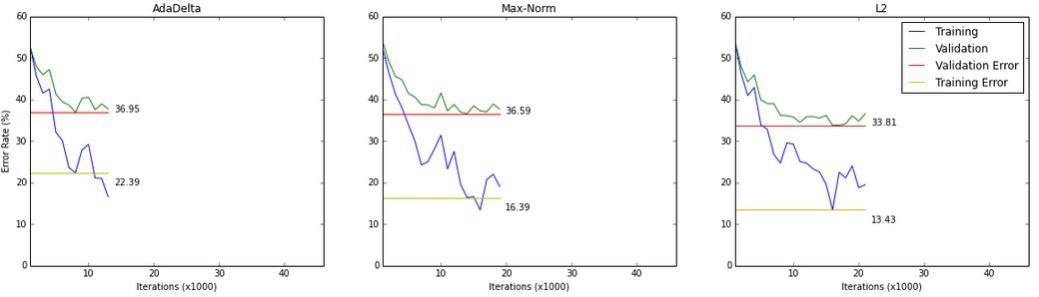
\includegraphics[width=0.8\linewidth]{images/6_overfit_max_l2_2}
\caption[]{Trainings- und Validierungsfehler während des Trainings auf dem reduzierten CIFAR-10B-Datensatz mittels AdaDelta-Methode, Max-Norm- und L2-Regularisierung}
\label{fig:6_overfit_max_l2}
\end{figure}


\subsubsection{Max-Norm-Regularisierung}
Im zweiten Experiment wird eine maximale Norm für die Gewichte festgelegt. Diese beträgt exemplarisch $ ||w||_2 <= 3  $ \cite[vgl.][]{Srivastava2014}.
Diese Art der Regularisierung hat weniger Einfluss auf das Training als die L2-Regularisierung. Dennoch wird der Validierungsfehler bei gleichzeitiger Verbesserung des Testfehlers um 1.58 \% etwas verschlechtert. Darüber hinaus ist der Testfehler in etwa gleich groß wie jener der L2-Regularisierung. Das Training mit Max-Norm-Regularisierung verhindert zu Beginn des Trainings eine Überanpassung, wie Abbildung \ref{fig:6_overfit_max_l2} zeigt. Das Training wird durch dies Regularisierung um 6 Epochen verlängert und \textit{Overfitting} tritt weiterhin sehr stark im Verlauf des Trainings auf.

\subsubsection{Dropout}
Die dritte betrachtete Methode zur Regularisierung ist das Dropout-Training. In diesen Experimenten werden zwei unterschiedliche Konfigurationen untersucht. Zuerst wird Dropout nur im Hidden-Layer des MLP angewandt. Anschließend wird die Dropout-Methode sowohl im Hidden-Layer des MLP als auch im letzten Convolution-Layer angewandt.
Als Dropout-Raten werden exemplarisch 0.3 \% und 0.5 \% untersucht (vgl. \cite{Srivastava2014}).
Im ersten Experiment wird Dropout nur im MLP verwendet. Bei beiden Dropout-Raten ist die Auswirkung auf das Training deutlich zu erkennen und der Unterschied zwischen Validierungs- und Testfehler fällt kleiner aus. Das bessere Ergebnis erreicht die Dropout-Rate von 0.3 \%, wodurch der Validierungsfehler auf 27.15 \% verschlechtert und der Testfehler gleichzeitig auf 33.13 \% verbessert wird. Ein Dropout von 0.5 \% führt hingegen zu einer Verschlechterung des Testfehler. Betrachtet man die Lernkurven in Abbildung \ref{fig:6_overfit_dropout} fällt auf, dass die Netze nach wie vor großes \textit{Overfitting} aufweisen.
Anders verhält es sich bei der zusätzlichen Anwendung von Dropout im letzten Convolution-Layer. Das Modell wird hierbei stärker regularisiert, was zu einer weiteren Verringerung des Abstandes zwischen den Fehlerraten führt. Allerdings verlängert sich die Trainingszeit deutlich. Hierbei führt eine Dropout-Rate von 0.3 \% zu einem etwas besseren Ergebnis als das Training ohne Regularisierung. Eine Dropout-Rate von 0.5 \% hingegen beschränkt das Modell sehr stark und das Ergebnis verschlechtert sich. Die Lernkurven weisen bei Dropout in mehreren Schichten jedoch deutlich weniger \textit{Overfitting} auf.

\begin{figure}
\centering
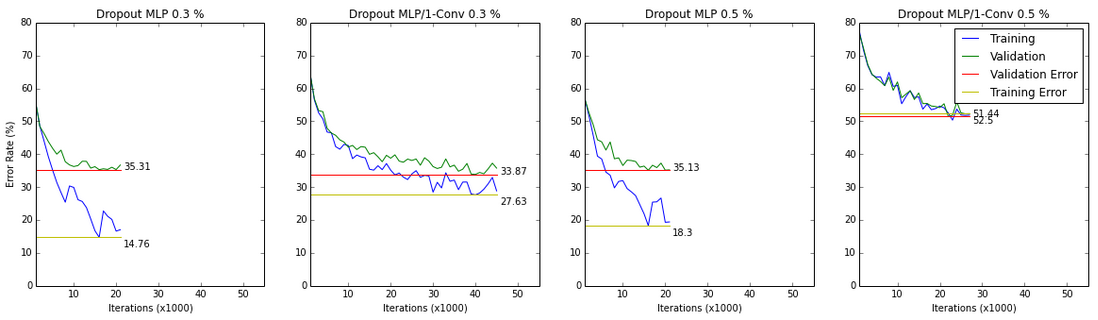
\includegraphics[width=1.0\linewidth]{images/6_overfit_dropout_2}
\caption[]{Trainings- und Validierungsfehler während des Trainings auf dem reduzierten CIFAR-10B-Datensatz mittels Dropout}
\label{fig:6_overfit_dropout}
\end{figure}

\subsubsection{Padding}
Die letzten Experimente zeigen, dass sowohl die L2-Regularisierung als auch das Dropout-Training zu einem kleinerem Abstand zwischen dem Validierungs- und Testfehler führen können. Die folgenden Experimente sollen die Auswirkung von Padding in den Convolution-Layern zeigen. Zusätzlich zum Padding wird die Dropout-Regularisierung mit einer Rate von 0.3 \% sowie die Max-Norm- und L2-Regularisierung aus den letzten Experimenten verwendet.
Durch Padding wird die Größe der Eingabe nur in den Pooling-Layern verringert. Damit erhöht sich die Dimension der Ausgabe des letzten Convolution-Layers von 64 auf 1024, was zu deutlich mehr trainierbaren Gewichten im MLP führt.\footnote{Hier wird in den Convolution-Layern aus Gründen der Implementierung Ausgabe-Padding eingesetzt und die CIFAR-10B-Eingaben werden entsprechend vor dem Training auf die Größe $36 \times 36$ vergrößert. Außerdem entfällt somit das Padding der Ausgabe des letzten Convolution-Layers.}

Wie das erste Experiment zeigt, steigt hierdurch die Kapazität des Modells deutlich und der Testfehler verbessert sich bei Dropout im MLP auf 29.69 \%. Im Vergleich zum Modell ohne Padding tritt am Ende außerdem ein größeres \textit{Overfitting} auf, durch Nutzung von Dropout allerdings weniger als im Modell ohne Regularisierung. Insgesamt zeigen die Lernkurven in Abbildung \ref{fig:6_overfit_padding} einen ähnlichen Verlauf wie jene des Trainings ohne Padding. Der größere Hidden-Layer im MLP wird oftmals durch die Max-Norm-Regularisierung regularisiert, was zu einem volatileren Verlauf im Trainingsfehler führt. 
Wird das Dropout-Training zusätzlich im letzten Convolution-Layer angewandt, wird das \textit{Overfitting} deutlich verringert, allerdings verschlechtert sich der Testfehler etwas.
Auffällig ist, dass das Modell hierbei weniger regularisiert wird als ohne Padding. Wird zusätzlich die L2-Regularisierung aktiviert, wird das \textit{Overfitting}, bei gleichzeitiger Verbesserung des Testfehlers und verkürzter Trainingszeit, deutlich reduziert.

\begin{figure}
\centering
\includegraphics[width=0.8\linewidth]{images/6_overfit_padding_2}
\caption[]{Trainings- und Validierungsfehler während des Trainings auf dem reduzierten CIFAR-10B-Datensatz mittels Dropout und Padding}
\label{fig:6_overfit_padding}
\end{figure}


\subsubsection{Modellkapazität}
Durch die Kombination von Padding, Dropout und Max-Norm- sowie L2-Regularisierung kann ein gewünschtes Ergebnis mit guter Generalisierung erzielt werden. Die folgenden Experimente sollen die Auswirkung der Modellkapazität und damit die Größe des Modells aufzeigen. Dazu werden zwei neue Modelle eingeführt, wobei das ein im Vergleich zum \textit{Net-7} eine Vergrößerung darstellt, das andere eine Verkleinerung. Beide neuen Netze verwenden ebenfalls Ausgabe-Padding.

\begin{table}
\centering
\begin{tabular}{c|c}
															& CIFAR-10B						 	\\ 
\hline \textit{Net-8} MLP/1-Conv 0.3 \% + L2/Max	& 	21.92/23.32/27.50 \%	 	(25 Ep.)	\\ %27.94
\hline \textit{Net-8} MLP/1-Conv 0.3 \% + Max		& 	16.15/21.20/27.55 \%	 	(27 Ep.)	\\
\hline \textit{Net-8} MLP 0.3 \% + Max				& 	13.30/13.26/27.84 \%	 	(25 Ep.)	\\
\hline \textit{Net-7-Small}	+ L2							& 	30.33/31.02/35.35 \% 		(37 Ep.)	\\
\hline Net-7 ohne Regularisierung							& 	20.86/21.99/36.65 \%		(12 Ep.)	\\
\hline \textit{Net-7-Small}	+ Max							& 	29.85/31.86/36.69 \% 		(20 Ep.)	\\
\end{tabular} 
\caption{Fehler auf den Trainings-/Validierungs-/Testdaten nach dem gesamten Training mit \textit{Net-7-Small} und \textit{Net-8} unter Verwendung verschiedener Methoden zur Regularisierung sortiert nach Testfehler}
\label{tab:6_regularisierung2}
\end{table}

Die Ergebnisse der einzelnen Experimente werden in Tabelle \ref{tab:6_regularisierung2} sortiert nach Testfehler aufgeführt. \\

\textit{Net-7-Small} \\
Das erste Netz, welches genutzt werden soll, besitzt keinen Hidden-Layer und die Anzahl der \textit{Feature-Maps} ist auf 20 reduziert. Es orientiert sich am Modell von \cite{Kaparthy2014}. Insgesamt besitzt dieses Netz lediglich 24.700 Gewichte, wobei die Architektur durch Padding einen weiteren Pooling-Layer nach dem letzten Convolution-Layer erlaubt.
Das Modell wird mit 20-20-20/10 abgekürzt und umfasst im Detail die folgenden sieben Schichten:
\begin{enumerate}
\setlength{\itemsep}{0pt}
\item Convolution-Layer: 20 \textit{Feature-Maps} mit $5 \times 5$ Filtermasken
\item Pooling-Layer:	$2 \times 2$ Filtermasken
\item Convolution-Layer: 20 \textit{Feature-Maps} mit $5 \times 5$ Filtermasken
\item Pooling-Layer:	$2 \times 2$ Filtermasken
\item Convolution-Layer: 20 \textit{Feature-Maps} mit $5 \times 5$ Filtermasken
\item Pooling-Layer:	$2 \times 2$ Filtermasken
\item Output-Layer: 10 Neuronen mit Cross-Entropy Fehlermaß
\end{enumerate}



\begin{figure}
\centering
\includegraphics[width=0.7\linewidth]{images/6_overfit_small_2}
\caption[]{Trainings- und Validierungsfehler während des Trainings auf dem reduzierten CIFAR-10B-Datensatz mittels \textit{Net-7-Small} sowie Max-Norm- und L2-Regularisierung}
\label{fig:6_overfit_small}
\end{figure}

Die Ergebnisse in Tabelle \ref{tab:6_regularisierung2} zeigen, dass das verkleinerte \textit{Net-7-Small} nahezu dasselbe Ergebnis wie das \textit{Net-7} erreicht. Gleichzeitig erreicht es eine bessere Generalisierung und benötigt eine kürzere Trainingszeit. Wird jedoch zusätzlich die L2-Regularisierung angewandt, verlängert sich die Trainingszeit hinsichtlich der durchlaufenen Epochen immens. Die Abbildung \ref{fig:6_overfit_small} zeigt auf, dass die Lernkurve hierbei einen flacheren Verlauf aufweist. Insgesamt verringert die Verkleinerung des Netzes das \textit{Overfitting} deutlich und führt bei zusätzlicher L2-Regularisierung zu einem besseren Testfehler.\\


\textit{Net-8} \\
Beim zweiten Netz werden die Anzahl der \textit{Feature-Maps} sowie die Anzahl der Neuronen im Hidden-Layer erhöht. Es stellt eine etwas kleinere Variante des Modells von \cite{Masci2011} dar. Insgesamt besitzt dieses Netz 510.100 Gewichte. Durch Padding erlaubt die Architektur, wie das \textit{Net-7-Small}, einen weiteren Pooling-Layer nach dem letzten Convolution-Layer, wodurch sich die Anzahl der Schichten auf acht erhöht.
Das Modell wird mit 100-100-100/100-10 abgekürzt und umfasst im Detail die folgenden acht Schichten:
\begin{enumerate}
\setlength{\itemsep}{0pt}
\item Convolution-Layer: 100 \textit{Feature-Maps} mit $5 \times 5$ Filtermasken
\item Pooling-Layer:	$2 \times 2$ Filtermasken
\item Convolution-Layer: 100 \textit{Feature-Maps} mit $5 \times 5$ Filtermasken
\item Pooling-Layer:	$2 \times 2$ Filtermasken
\item Convolution-Layer: 100 \textit{Feature-Maps} mit $5 \times 5$ Filtermasken
\item Pooling-Layer:	$2 \times 2$ Filtermasken
\item Hidden-Layer: 100 Neuronen
\item Output-Layer: 10 Neuronen mit Cross-Entropy Fehlermaß
\end{enumerate}


Mit dem vergrößerten Netz steigt die Kapazität des Netzes im Vergleich zum \textit{Net-7} mit Padding nochmals, was zu den besseren Fehlerraten führt, die in Tabelle \ref{tab:6_regularisierung2} aufgeführt sind. Das Netz weist am Ende ebenfalls ein großes \textit{Overfitting} auf und die Lernkurven in Abbildung \ref{fig:6_overfit_big} weisen einen ähnlichen Verlauf wie die Kurven im \textit{Net-7} auf. Wird das Netz mit L2-Regularisierung trainiert, verbessert sich die Generalisierung und das Netz erreicht den besten Testfehler im Rahmen dieser Experimente. 

\begin{figure}
\centering
\includegraphics[width=0.8\linewidth]{images/6_overfit_big_2}
\caption[]{Trainings- und Validierungsfehler während des Trainings auf dem reduzierten CIFAR-10B-Datensatz mittels \textit{Net-8} mit Max-Norm- und L2-Regularisierung sowie Dropout}
\label{fig:6_overfit_big}
\end{figure}

	
\section{Visualisierung}
Neben der Darstellung der Filtermasken existieren zur Visualisierung weitere nützliche Methoden.
Im folgenden Teil soll die Anwendung zweier zentraler Techniken zur Visualisierung von CNNs gezeigt werden. Einerseits die sogenannte Neuronen-Visualisierung zur Rekonstruktion der Aktivierung eines beliebigen Neurons, andererseits die t-SNE zur Dimensionsreduktion. Darüber hinaus werden mittels des Convolutional Autoencoders die Aktivierungen im CNN untersucht.
	

\subsection{Neuronen-Visualisierung}
Mit der Neuronen-Visualisierungen können einzelne aktivierte \textit{Feature-Maps} in den Eingaberaum zurück propagiert werden. Bis auf wenige Anpassungen, funktioniert diese analog zum \textit{Backward Pass} des Backpropagation-Algorithmus.


\begin{figure}
\centering
\includegraphics[width=1.0\linewidth]{images/6_visualize_mnist}
\caption[]{Visualisierung der neun stärksten Aktivierungen im \textit{LeNet 5+} mit der Methode von \cite{Zeiler2014} auf den gesamten Testdaten:  Erste \textit{Feature-Map} in der zweiten Schicht (links) und erste \textit{Feature-Map} in der vierten Schicht (rechts)}
\label{fig:6_vis_mnist}
\end{figure}


Im folgenden soll die Methode von \cite{Zeiler2014} angewandt werden, um beispielhafte Neuronen zu visualisieren. Abbildung \ref{fig:6_vis_mnist} zeigt je eine \textit{Feature-Map} der zweiten sowie der vierten Schicht eines mit MNIST-Daten trainierten \textit{LeNet 5+}. Die \textit{Feature-Map} der ersten Schicht fungiert eindeutig als Kantendetektor, was auch bei der Betrachtung der Filtermasken in Abbildung \ref{fig:6_filters_mnist} plausibel erscheint. Interessanter erscheint die \textit{Feature-Map} der vierten Schicht. Diese scheint gerade Kanten besonders zu detektieren, was bei den Ziffern fünf und sieben besonders auffällt.



Wird dieselbe Methode auf ein mit CIFAR-10B-Daten trainiertes \textit{Net-8} angewandt, ergeben sich die Rekonstruktionen in Abbildung \ref{fig:6_vis_cifar}, wobei jeweils der V-Kanal dargestellt ist. Hier werden jeweils zwei \textit{Feature-Maps} in der zweiten und vierten Schicht gezeigt. Wie auch im \textit{LeNet 5+} fungieren die Filtermasken der zweiten Schicht als Kantendetektoren. Darüber hinaus detektieren sie bei Farbbildern die Tönung des Bildes. Die obere \textit{Feature-Map} der vierten Schicht hingegen scheint, bis auf zwei Ausnahmen, Schiffe zu detektieren. Betrachtet man die Rekonstruktionen, ist erkennbar, dass besonders die länglichem Kanten erkannt werden. Außerdem weist die Rekonstruktion der Aktivierung des oberen Autos starke Ähnlichkeit zu einem Boot auf. Die zweite \textit{Feature-Map} detektiert augenscheinlich längliche Objekte. Diese lassen sich alleine mit dieser \textit{Feature-Map} nicht einzelnen Klassen zuordnen. Dennoch weist diese eine gewissen Relevanz auf, da sowohl drei sehr ähnliche Tarnkappen-Flugzeuge und drei sitzende Katzen detektiert werden. 

\begin{figure}
\centering
\includegraphics[width=1.0\linewidth]{images/6_visualize_cifar}
\caption[]{Visualisierung der neun stärksten Aktivierungen im \textit{Net-8}  mit der Methode von \cite{Zeiler2014} auf den gesamten Testdaten: Erstes und neuntes Neuron in der zweiten Schicht (links) und erstes und neuntes Neuron in der vierten Schicht (rechts)}
\label{fig:6_vis_cifar}
\end{figure}


\subsection{t-SNE-Methode}
Die t-SNE-Methode von \cite{Laurens2008} kann wie die Hauptkomponentenanalyse (PCA) zur Dimensionsreduktion eingesetzt werden. Im Unterschied zur PCA berücksichtigt diese bei der Reduktion alle Hauptkomponenten. An dieser Stelle wird t-SNE verwendet, um die von den Convolution-Layern extrahierten Merkmale im 2D-Bildraum zu visualisieren. Die t-SNE wird im Folgenden ausgehend von den ersten 50 Hauptkomponenten 1000 Iterationen lange gerechnet.

Abbildung \ref{fig:6_tsne_mnist} zeigt zufällige 2500 originale sowie durch das CNN transformierte MNIST-Beispiele in einem Streudiagramm. Es ist deutlich erkennbar, dass die zehn Klassen nach den beiden Convolution-Layern des \textit{LeNet 5+} kompaktere Gruppen bilden. Dies ermöglicht eine bessere Trennung der Daten im nachfolgenden mit abschließender Softmax-Regression.

\begin{figure}
\centering
\includegraphics[width=0.9\linewidth]{images/6_tsne_mnist}
\caption[]{Visualisierung von 2500 MNIST-Beispielen mit t-SNE im Original (links) und nach der vierten Schicht des trainierten \textit{LeNet 5+} (rechts)}
\label{fig:6_tsne_mnist}
\end{figure}

Für die Visualisierung der CIFAR-10B-Daten wird eine andere Methode gewählt. An Stelle des Streudiagramms werden die einzelnen Beispiele selbst dargestellt. Die Abbildungen \ref{fig:6_tsne_cifara} und \ref{fig:6_tsne_cifarb} zeigt 1000 originale sowie durch das CNN transformierte CIFAR-10B-Beispiele. Hierbei fällt zum einen auf, dass die Originale eindeutig anhand des Hintergrunds getrennt werden, während die Farbtöne in der Variante des CNNs etwas verwaschener sind. Darüber hinaus sind in der Punktwolke mit den extrahierten Merkmalen Lücken erkennbar. Bei genauer Betrachtung kann, beispielsweise anhand des grünen Autos im Original rechts in der Mitte, die Gruppenbildung nach Inhalt, statt nach Hintergrund oder Farbtons  festgestellt werden. Das genannte grüne Auto befindet sich nach Anwendung der Convolution-Layer bei den anderen Autos links in der Mitte. Außerdem ist die rötliche Gruppe unten-rechts bei Anwendung der t-SNE mit extrahierten Merkmalen aufgelöst.


\begin{figure}[H]
\centering
\includegraphics[width=0.8\linewidth]{images/6_cifar_tsne_combined_white_small2a}
\caption[]{Visualisierung von 1000 CIFAR-10-Beispielen mit t-SNE im Original}
\label{fig:6_tsne_cifara}
\end{figure}

\begin{figure}[H]
\centering
\includegraphics[width=0.8\linewidth]{images/6_cifar_tsne_combined_white_small2b}
\caption[]{Visualisierung von 1000 CIFAR-10B-Beispielen mit t-SNE nach der sechsten Schicht des trainierten \textit{Net-8}}
\label{fig:6_tsne_cifarb}
\end{figure}
		

\subsection{Autoencoder-Visualisierung}		
Der eingangs zum unüberwachten Vortraining untersuchte Convolutional Autoencoder kann ebenso zur Visualisierung verwendet werden. Dazu wird zunächst die Aktivierung für Beispieldaten in einer bestimmten Schicht berechnet. Anschließend wird diese Aktivierung anstatt des Verfahrens von \cite{Zeiler2014} mit dem Decoder des Convolutional Autoencoders in den Bildraum zurück propagiert. Die Schichten mit Max-Pooling werden zwecks Umkehrbarkeit mit Average-Pooling ausgestattet.

\begin{figure}[H]
\centering
\includegraphics[width=0.4\linewidth]{images/6_visualize_mnist_autoenc}
\caption[]{Zufälligen MNIST-Beispiele im Original (links) und visualisiert mit der Autoencoder-Methode auf Basis der Aktivierungen in der vierten Schicht im \textit{LeNet 5+} (rechts)}
\label{fig:6_visualize_mnist_autoenc}
\end{figure}

Die Abbildung \ref{fig:6_visualize_mnist_autoenc} zeigt dieses Verfahren angewandt auf zufällige MNIST-Beispiele, wobei die Rekonstruktionen auffällig gut sind. Durch die ReLu-Aktivierung verschwinden außerdem negative Werte und der Hintergrund ist im Unterschied zur Methode von \cite{Zeiler2014} schwarz. Dies ist eine sehr interessante Feststellung, da die verschiedenen Filtermasken nicht mittels Autoencoder trainiert wurden. Darüber hinaus erklärt dies, warum unüberwachtes Vortraining im Deep Learning eine geeignete Methode für das Training der Filtermasken darstellt. 
	
\subsubsection{Maskierung von Merkmalen}
\begin{figure}
\centering
\includegraphics[width=0.8\linewidth]{images/6_visualize_mnist_autoenc2}
\caption[]{Mittels der Autoencoder-Methode visualisierte, zufällige MNIST-Beispiele mit verdeckter zehnter \textit{Feature-Map} (links), zwanzigster (mitte-links), den ersten vier (mitte-rechts) und allen ab der vierten \textit{Feature-Map} (rechts) auf Basis der Aktivierungen in der vierten Schicht im \textit{LeNet 5+}}
\label{fig:6_visualize_mnist_autoenc2}
\end{figure}

Die beschriebene Methode erlaubt ein weiteres Experimente hinsichtlich der Aktivierungen einer Schicht.
Die Abbildung \ref{fig:6_visualize_mnist_autoenc2} zeigt vier mittels Autoencoder rekonstruierte Aktivierungen. Bei den ersten Rekonstruktionen wurde die zehnte \textit{Feature-Map} der vierten Schicht verdeckt, bei den zweiten Rekonstruktionen die zwanzigste, bei den dritten die ersten vier und bei den vierten alle, außer die ersten vier. Interessanterweise sehen die ersten drei Rekonstruktionen nahezu identisch aus, während jene der vierten Abbildung kaum mehr zu erkennen sind. Dies zeigt, dass sich einzelne \textit{Feature-Maps} nicht an einzelnen Trainingsbeispielen orientieren, sondern, im Sinne der \textit{Distributed Representation}, die Kombination aus Merkmalen wichtig ist \cite[vgl.][]{Hinton1986}.

In Abbildung \ref{fig:6_cov_mnist_1_8_18} sind mehrere Kovarianzen mit spaltenweise addiertem Mittelwert dargestellt. Im ersten Bild wird die Kovarianzmatrix aller Aktivierungen der vierten Schicht mit der Ziffer 1 berechnet, im zweiten jene der Ziffer 8 und im dritten die Kombination der Ziffern 1 und 8. Insgesamt besitzt die vierte Schicht 800 Merkmale, wobei jede \textit{Feature-Map} davon 16 bündelt.	
Zunächst fällt auf, dass bei der Ziffer 1 der Mittelwert der 21. \textit{Feature-Map} die anderen dominiert. Außerdem ist die Information über mehrere Merkmale verteilt, was die erhöhten Kovarianzen innerhalb der Zeile zeigen. Analog verhält es sich bei den Aktivierungen der Ziffer 8. Darüber hinaus sind in der Kombination der Ziffern entsprechend beide Muster in den Aktivierungen erkennbar, wobei die Mittelwerte der 21. und 22. \textit{Feature-Maps} dominieren.


\begin{figure}
\centering
\includegraphics[width=0.6\linewidth]{images/6_cov_mnist_1_8_18}
\caption[]{Kovarianzmatrix der Aktivierungen der vierten Schicht im \textit{LeNet 5+} auf Basis aller MNIST-Beispiele mit der Ziffer 1 (links), der Ziffer 8 (mitte) und den Ziffern 1 und 8 (rechts)}
\label{fig:6_cov_mnist_1_8_18}
\end{figure}

\begin{figure}
\centering
\includegraphics[width=0.6\linewidth]{images/6_visualize_mnist_autoenc_8_1}
\caption[]{Neun zufälligen MNIST-Beispielen mit der Ziffer 1 und 7 im Original (links) und visualisiert mit der Autoencoder-Methode auf Basis der gemittelten Merkmalen (mitte-rechts) und addierten Merkmalen (rechts) nach der vierten Schicht im \textit{LeNet 5+}}
\label{fig:6_visualize_mnist_autoenc_8_1}
\end{figure}


\subsubsection{Kombination von Merkmalen}

Im letzten Experiment konnte festgestellt werden, dass mehrere \textit{Feature-Maps} bei ähnlichen Eingaben korrelieren. In einem abschließenden Experiment soll die Kombination der Aktivierungen in der vierten Schicht und folglich eine Merkmalskombination visualisiert werden. Die Abbildung \ref{fig:6_visualize_mnist_autoenc_8_1} zeigt einerseits die originalen Eingaben und andererseits, auf Basis der kombinierten Merkmale der Ziffern 1 und 8, die entsprechenden Rekonstruktionen. In den Rekonstruktionen ist eindeutig erkennbar, dass die Mischung von Merkmalen zu einer entsprechenden Vermischung im Eingaberaum führt und somit entartete Kombinationen aus den Ziffern 1 und 8 entstehen. Dabei hat interessanterweise die Stärke der Aktivierung wenig Einfluss auf das Ergebnis, was der Vergleich der Rekonstruktionen mit und ohne Mittelung zeigt.

Weiterführend können auf Basis der Aktivierungen, analog zum Verfahren von \cite{Vincent2010}, auch mittels Convolutional Autoencoder synthetische \textit{Samples} erzeugt werden. Diese Methode wird allerdings in dieser Arbeit nicht näher betrachtet.




%\begin{figure}
%\centering
%\includegraphics[width=0.6\linewidth]{images/6_cov_mnist_hidden}
%\caption[]{25 zufälligen MNIST-Beispielen im Original (links) und visualisiert mit der %Autoencoder-Methode auf Basis der Aktivierungen in der vierten Schicht im \textit{LeNet 5+} (rechts)}
%\label{fig:6_cov_mnist_hidden}
%\end{figure}


	
		
% erstmal nicht beachtet\hline Dropout ALL 0.3 \% + Max								& 	51.07/49.94 \%	 	(xx Ep.)	\\
% no Pooling \hline Dropout ALL 0.3 \% + Max-Norm + Pad/Mask 				& 	51.64/51.93 \%	 	(xx Epochen)	\\
% no Pooling \hline Dropout MLP 0.3 \% + Max-Norm + Padding					& 	19.74/31.79 \%	 	(xx Epochen)	\\
%\hline \textit{7-Net}-Small	+ L2/Max-Norm + Padding	+ Long				& 	30.36/35.46 \% 		(xx Epochen)	\\
% erstnal nicht beachtet \hline L2-Regularisierung + No MLP					& 	27.73/37.75 \% 		(xx Epochen)	\\
% erstmal nich beachtet \hline \textit{7-Net}-Big Dropout MLP 0.3 \% + Max-Norm 			& 	00.00/00.00 \%	 	(xx Epochen)	\\
%\hline \textit{7-Net}-Big Dropout MLP 0.3 \% + Max-Norm + Padding + Long	& 	00.00/00.00 \%	 	(xx Epochen)	\\		
		
\chapter{Zusammenfassung}
%- Fazit 												( 3 Seiten)	( 3 Seiten)	
Das Feld von Deep Learning und Convolutional Neural Networks (CNNs) fasst sehr viele interessante Facetten. In dieser Arbeit wurden die Bereiche des überwachten neuronalen Lernmodells zur Klassifikation und Regression aufbereitet. Aufbauend auf das klassische Multilayer Perceptron (MLP), wurden die speziellen Convolutional Neural Networks eingeführt. Diese lassen sich wie gewohnte mehrschichtige Netze mittels Backpropagation-Algorithmus trainieren, bieten jedoch aufgrund ihrer Architektur große Vorteile gegenüber MLPs. Hierbei ist besonders deren Eigenschaft hervorzuheben, lokale Merkmale im Eingaberaum zu berücksichtigen. Darüber hinaus stellt die Entkopplung der Dimensionalität der Eingabe von der Anzahl der trainierbaren Gewichte einen weiteren Vorteil der Convolutional Neural Networks dar. In den darauffolgenden Kapiteln wurde aufgezeigt, warum tiefe Netze schwer zu trainieren sind und wie moderne Methoden im Bereich Deep Learning dabei helfen können, diese Schwierigkeiten zu überwinden. Als die beiden wichtigsten Beispiele wurden das \textit{Overfitting} sowie der \textit{Vanishing Gradient}-Effekt vorgestellt. Als Einstieg in das Thema seien an dieser Stelle die Arbeiten von \cite{Bengio2009} und \cite{Bengio2012} empfohlen. Im weiteren Verlauf der Arbeit wurde, basierend auf den vorgestellten Methoden, ein eigenes CNN implementiert und mit diversen Experimenten auf Richtigkeit überprüft. 
In diesem Kapitel werden die Ergebnisse nochmals zusammengefasst und ein Ausblick auf weitere mögliche Forschungstätigkeit im Umfeld von CNNs gegeben.
							

\section{Ergebnisse}
Der im Rahmen dieser Arbeit entwickelte CPU-basierte Prototyp eines CNN konnte durch die Experimente bereits seine Leistungsfähigkeit unter Beweis stellen. Neben den aktuellen Methoden im Deep Learning zur Initialisierung und Optimierung, sind auch nützliche Methoden zur Visualisierung sowie zum unüberwachten Vortraining implementiert worden. Neben einer Python-Schnittstelle weist das \textit{ConvNetCPP} wenige Abhängigkeiten auf und kann so leicht auf anderen Systemen eingesetzt werden.

Für die Anwendung ist als Vorverarbeitungsstufe die Zentrierung der Daten besonders wichtig, da ansonsten die Logistische Sigmoidfunktion oder der Tangens Hyperbolicus schnell sättigen können. Auch der HSV-Farbraum liefert konsistent etwas bessere Ergebnisse als der RGB-Farbraum. Im Rahmen der Initialisierung kann gefolgert werden, dass die Initialisierung der ersten Schicht durch unüberwachtes Vortraining nicht ausreicht, um die schlechte Initialisierung des restlichen Netzes zu reparieren. Ebenso scheint die Standardabweichung von $\sigma = 0.01$ der Standard-Initialisierung für das CIFAR-10-Problem zu klein zu sein. Dies zeigt auch das Experiment, bei dem ein sonst Xavier-initialisiertes Netz vortrainiert wird. Hierbei fällt der Validierungsfehler auf CIFAR-10A nach der ersten Epoche von 63 \%, bei reiner Xavier-Initialisierung, auf den besseren Wert von 61.8 \%. Insgesamt werden die Gewichte des \textit{Net-7} bei Xavier-Initialisierung mit $\sigma \approx 0.035$ in den Convolution-, $\sigma \approx 0.18$  im Hidden- und $\sigma \approx 0.16$ im Output-Layer initialisiert. 

Während der Experimente wurde stets eine \textit{Early Stopping Patience} von fünf Epochen verwendet und das Training anschließend mit den gesamten Daten für maximal fünf weitere Epochen fortgesetzt. Dies bedeutet eine starke Beschränkung der Trainingszeit, was sich gerade beim Training mit den CIFAR-10-Daten bemerkbar macht. Hier wirken durch die kurze Trainingszeit die Filtermasken noch recht verrauscht. Trotz der Beschränkung erreicht das \textit{LeNet 5+} einen bemerkenswerten Testfehler von 0.61 \%. Wird die Wartezeit beim \textit{Early Stopping} auf 15 Epochen erhöht, erreicht auch das \textit{Net-7} mit \textit{Padding} und angewandtem Dropout von 0.3 \% im MLP und dem letzten Convolution-Layer nach 72 Epochen einen Testfehler von 25.02 \%. Das stellt im Vergleich zum deutlich größeren Netz von \cite{Masci2011} (100-150-200/300-10) einen plausiblen Wert dar.

Zusammenfassend lassen sich folgende Folgerungen aus den Experimenten ableiten:

\begin{itemize}
\item Die Zentrierung der Daten ist obligatorisch.
\item Padding erhöht die Kapazität und verbessert die Performanz ohne markant größeren Rechenaufwand.
\item Max-Norm-Regularisierung verhindert \textit{Overfitting} zu Beginn des Trainings und beschleunigt letzteres.
\item Dropout und L2-Regularisierung sind gute Verfahren zur Verbesserung der Generalisierung.
\item Die L2-Regularisierung dominiert die Max-Norm-Regularisierung.
\item Die Anwendung einer starken Regularisierung verlängert die Trainingszeit immens.
\item Ein kleiner dimensioniertes Netz kann gleichwertige Ergebnisse wie ein großes, nicht regularisiertes Netz erzielen.
\item Methoden zur Visualisierung sind gute Werkzeuge, um erlernte Merkmale sichtbar zu machen und die Funktionsweise von CNNs zu erklären.
\end{itemize}

Im Rahmen der Experimente kamen bewährte Standardwerte für die Hyperparameter zum Einsatz. Für spezielle Probleme müssen diese durch Kreuzvalidierung oder ähnliche Verfahren bestimmt werden. Ein guter Ausgangspunkt für die Optimierung sind das AdaDelta-Verfahren oder das SGD-ähnliche Nesterov-Momentum ohne adaptive Lernrate, da diese das Training stark beschleunigen können. 
Für die Bestimmung der optimalen Hyperparameter ist die Rechenkapazität eine restriktive Größe. So ist das Training der MNIST-Daten mit \textit{ConvNetCPP} auf dem \textit{LeNet 5+} mit etwa einer Stunde CPU-Zeit pro Epoche noch recht schnell. Auf dem CIFAR-10-Datensatz in Kombination mit dem \textit{Net-7} dauert das Training mit etwa drei Stunden CPU-Zeit pro Epoche jedoch sehr lange. Damit ist das Training größerer Netze, wie des CIFAR-10-Netz von \cite{Masci2011}, sehr zeitaufwändig. Auch sind längere Trainingszeiten von 280 Epochen für das CIFAR-10-Netz von \cite{Zeiler2013b} nur schwer möglich. 
In der Praxis sollte mit einem kleinen Netz gestartet und dieses sukzessive ausgebaut werden, bis der Validierungsfehler nicht weiter sinkt oder der Trainingsfehler den Wert Null erreicht. Anschließend sollten die Fehlerraten von Trainings- und Validierungsdaten mit den beschriebenen Techniken der Regularisierung angeglichen werden, um eine bestmögliche Generalisierung zu ermöglichen.

\section{Ausblick}
Betrachtet man die Laufzeiten der verschiedenen Experimente, wird klar, dass auch ein optimiertes CPU-basiertes CNN für große Datensätze und tiefe Architekturen nicht geeignet ist. Durch die Reduktion der 2D-Faltung auf eine Matrix-Matrix-Multiplikation (GEMM), wird die meiste Rechenzeit für solcherlei Multiplikationen aufgewendet. Diese kann durch eine entsprechende GPU-Implementierung deutlich reduzieren werden. Darüber hinaus lässt sich das Training eines Modells durch spezielle Modell-Parallelisierung ebenfalls beschleunigen \cite[vgl.][]{Krizhevsky2014}. Die Beschleunigungen sind auch hinsichtlich erweiterter Trainingsdaten (\textit{Data Augmentation}) zur Steigerung der Performanz von Bedeutung.

Die Performanz eines CNN lässt sich auch durch weitere spezielle Schichten verbessern. An dieser Stelle sei auf die speziellen \textit{Max-Out}-Netze von \cite{Goodfellow_maxout_2013} und die \textit{DropConnect}-Netze von \cite{Zeiler2013} verwiesen, welche besonders auf dem CIFAR-10-Datensatz hervorragende Ergebnisse liefern.
Weiterhin existieren Schichten, welche nach jedem Convolution-Layer zur lokalen Kontrastnormalisierung eingesetzt werden. Dies verhindert, dass einzelne \textit{Feature-Maps} die Aktivierungen der Schicht dominieren (vgl. \cite{Jarrett2009}).
Darüber hinaus zeigen neuere Netze eine weitere Adaption der üblichen Convolutional-Layer. Meist werden diese als \textit{locally connected} oder LC-Layer bezeichnet (vgl. \cite{Nouri2013} und \cite{LeRanzato2012}). Solche Schichten zeichnen sich dadurch aus, dass lokale rezeptive Felder zwar definiert, die Parameter zwischen den einzelnen Feldern allerdings nicht geteilt werden. Der ursprüngliche Vorteil von CNNs durch \textit{Parameter Sharing} das Modell zu beschränken wird hierdurch verworfen, allerdings kann die größere Kapazität durch anderweitige Regularisierung dennoch zu besseren Ergebnissen führen (vgl. \cite{Hinton2012} und \cite{Krizhevsky2012}).
In diesem Zusammenhang sind auch weitere Experimente im Rahmen des unüberwachten Vortrainings von Interesse, in denen beispielsweise das gesamte CNN mittels eines Stacked Denoising Autoencoders (SDA) initialisiert wird.

Im Allgemeinen ist das Training eines zufällig initialisierten Netzes, beispielsweise auf Basis der ImageNet-Daten \cite[vgl.][]{ImageNet2015}, sehr zeitaufwändig. An dieser Stelle soll deshalb noch ein Hinweis auf eine Ablage bereits trainierter Netze für Caffe gegeben werden \cite[vgl.][]{Caffe2014}, welche für weitere Experimente von Interesse sein kann.\footnote{Projektseite von Caffe: \url{https://github.com/BVLC/caffe} (22.09.2015)}  Diese Netze können beispielsweise zur Merkmalsextraktion oder für Feintuning im Rahmen des Transferlernens eingesetzt werden.

Insgesamt zeigt sich, dass Convolutional Neural Networks in Verbindung mit Methoden des Deep Learning ein ausgezeichnetes Modell für die Klassifikation und Regression von Daten mit lokalen Merkmalen im Eingaberaum darstellen. Insbesondere die Möglichkeit Vorwissen über die Struktur der Daten einzubetten bietet eine große Vielfalt an Optimierungsmöglichkeiten. Dennoch ist die Suche nach den optimalen Hyperparametern schwierig und die Suche nach Fehlern oftmals zeitintensiv. Besonders hier gilt es neue Verfahren zu entwickeln, um die Handhabung solcher Modelle zukünftig einfacher zu gestalten.



\addcontentsline{toc}{chapter}{Literaturverzeichnis}
\bibliography{bibtex/literatur}




\end{document}
